% Options for packages loaded elsewhere
\PassOptionsToPackage{unicode}{hyperref}
\PassOptionsToPackage{hyphens}{url}
\PassOptionsToPackage{dvipsnames,svgnames,x11names}{xcolor}
%
\documentclass[
  12pt,
  letterpaper,
]{article}

\usepackage{amsmath,amssymb}
\usepackage{setspace}
\usepackage{iftex}
\ifPDFTeX
  \usepackage[T1]{fontenc}
  \usepackage[utf8]{inputenc}
  \usepackage{textcomp} % provide euro and other symbols
\else % if luatex or xetex
  \usepackage{unicode-math}
  \defaultfontfeatures{Scale=MatchLowercase}
  \defaultfontfeatures[\rmfamily]{Ligatures=TeX,Scale=1}
\fi
\usepackage{lmodern}
\ifPDFTeX\else  
    % xetex/luatex font selection
  \setmainfont[Numbers=Proportional,Numbers=OldStyle]{Linux Libertine O}
  \setmathfont[]{Libertinus Math}
\fi
% Use upquote if available, for straight quotes in verbatim environments
\IfFileExists{upquote.sty}{\usepackage{upquote}}{}
\IfFileExists{microtype.sty}{% use microtype if available
  \usepackage[]{microtype}
  \UseMicrotypeSet[protrusion]{basicmath} % disable protrusion for tt fonts
}{}
\usepackage{xcolor}
\usepackage[top=1in,bottom=1in,left=1in,right=1in]{geometry}
\setlength{\emergencystretch}{3em} % prevent overfull lines
\setcounter{secnumdepth}{-\maxdimen} % remove section numbering


\providecommand{\tightlist}{%
  \setlength{\itemsep}{0pt}\setlength{\parskip}{0pt}}\usepackage{longtable,booktabs,array}
\usepackage{calc} % for calculating minipage widths
% Correct order of tables after \paragraph or \subparagraph
\usepackage{etoolbox}
\makeatletter
\patchcmd\longtable{\par}{\if@noskipsec\mbox{}\fi\par}{}{}
\makeatother
% Allow footnotes in longtable head/foot
\IfFileExists{footnotehyper.sty}{\usepackage{footnotehyper}}{\usepackage{footnote}}
\makesavenoteenv{longtable}
\usepackage{graphicx}
\makeatletter
\def\maxwidth{\ifdim\Gin@nat@width>\linewidth\linewidth\else\Gin@nat@width\fi}
\def\maxheight{\ifdim\Gin@nat@height>\textheight\textheight\else\Gin@nat@height\fi}
\makeatother
% Scale images if necessary, so that they will not overflow the page
% margins by default, and it is still possible to overwrite the defaults
% using explicit options in \includegraphics[width, height, ...]{}
\setkeys{Gin}{width=\maxwidth,height=\maxheight,keepaspectratio}
% Set default figure placement to htbp
\makeatletter
\def\fps@figure{htbp}
\makeatother

% -----------------------
% CUSTOM PREAMBLE STUFF
% -----------------------

% -----------------
% Typography tweaks
% -----------------
% Indent size
\setlength{\parindent}{0.5in}
\setlength{\leftmargin}{0.5in}

% Fix widows and orphans
\usepackage[all,defaultlines=2]{nowidow}

% List things
\usepackage{enumitem}
% Same document-level indentation for ordered and ordered lists
\setlist[1]{labelindent=\parindent}
\setlist[itemize]{leftmargin=*}
\setlist[enumerate]{leftmargin=*}

% Wrap definition list terms
% https://tex.stackexchange.com/a/9763/11851
\setlist[description]{style=unboxed}


% For better TOCs
\usepackage{tocloft}

% Remove left margin in lists inside longtables
% https://tex.stackexchange.com/a/378190/11851
\AtBeginEnvironment{longtable}{\setlist[itemize]{nosep, wide=0pt, leftmargin=*, before=\vspace*{-\baselineskip}, after=\vspace*{-\baselineskip}}}

% For fancy ORCID links
\usepackage{orcidlink}

% Indent all first paragraphs because APA wants that
\usepackage{indentfirst}


% -----------------
% Title block stuff
% -----------------

% Abstract
\usepackage{abstract}
\renewcommand{\abstractnamefont}{\normalfont\normalsize\bfseries}
\renewcommand{\abstracttextfont}{\normalsize}
\setlength{\absleftindent}{\parindent}
\setlength{\absrightindent}{\parindent}


% Keywords
\providecommand{\keywords}[1]{\textbf{\textit{Keywords---}}#1}
  
% Title
\usepackage{titling}
\setlength{\droptitle}{2\baselineskip}
\pretitle{\begin{center}\normalfont\normalsize\bfseries}
\posttitle{\par\end{center}\vspace{2\baselineskip}}


% ------------------
% Section headings
% ------------------
\usepackage{titlesec}
\titleformat*{\section}{\center\normalsize\bfseries}
\titleformat*{\subsection}{\normalsize\bfseries}
\titleformat*{\subsubsection}{\normalsize\bfseries\itshape}
\titleformat{\paragraph}[runin]{\bfseries}{\theparagraph.}{3pt}{\space}[.]
\titleformat{\subparagraph}[runin]{\bfseries\itshape}{\thesubparagraph.}{3pt}{\space}[.]

% \titlespacing{<command>}{<left>}{<before-sep>}{<after-sep>}
% Starred version removes indentation in following paragraph
\titlespacing*{\section}{0em}{2em}{0em}
\titlespacing*{\subsection}{0em}{1em}{0em}
\titlespacing*{\subsubsection}{0em}{0em}{0em}
\titlespacing*{\paragraph}{\parindent}{1ex}{1em}
\titlespacing*{\subparagraph}{\parindent}{1ex}{1em}


% -----------
% Footnotes
% -----------
% NB: footmisc has to come after biblatex because of conflicts
\usepackage[bottom]{footmisc}
\renewcommand*{\footnotelayout}{\footnotesize}

\addtolength{\skip\footins}{12pt}  % vertical space between rule and main text
\setlength{\footnotesep}{16pt}  % vertical space between footnotes


% ----------
% Captions
% ----------
\usepackage[font=normalsize]{caption}


% ---------------------------
% END CUSTOM PREAMBLE STUFF
% ---------------------------
\usepackage{booktabs}
\usepackage{longtable}
\usepackage{array}
\usepackage{multirow}
\usepackage{wrapfig}
\usepackage{float}
\usepackage{colortbl}
\usepackage{pdflscape}
\usepackage{tabu}
\usepackage{threeparttable}
\usepackage{threeparttablex}
\usepackage[normalem]{ulem}
\usepackage{makecell}
\usepackage{xcolor}
\usepackage{caption}
\makeatletter
\@ifpackageloaded{tcolorbox}{}{\usepackage[skins,breakable]{tcolorbox}}
\@ifpackageloaded{fontawesome5}{}{\usepackage{fontawesome5}}
\definecolor{quarto-callout-color}{HTML}{909090}
\definecolor{quarto-callout-note-color}{HTML}{0758E5}
\definecolor{quarto-callout-important-color}{HTML}{CC1914}
\definecolor{quarto-callout-warning-color}{HTML}{EB9113}
\definecolor{quarto-callout-tip-color}{HTML}{00A047}
\definecolor{quarto-callout-caution-color}{HTML}{FC5300}
\definecolor{quarto-callout-color-frame}{HTML}{acacac}
\definecolor{quarto-callout-note-color-frame}{HTML}{4582ec}
\definecolor{quarto-callout-important-color-frame}{HTML}{d9534f}
\definecolor{quarto-callout-warning-color-frame}{HTML}{f0ad4e}
\definecolor{quarto-callout-tip-color-frame}{HTML}{02b875}
\definecolor{quarto-callout-caution-color-frame}{HTML}{fd7e14}
\makeatother
\makeatletter
\@ifpackageloaded{caption}{}{\usepackage{caption}}
\AtBeginDocument{%
\ifdefined\contentsname
  \renewcommand*\contentsname{Table of contents}
\else
  \newcommand\contentsname{Table of contents}
\fi
\ifdefined\listfigurename
  \renewcommand*\listfigurename{List of Figures}
\else
  \newcommand\listfigurename{List of Figures}
\fi
\ifdefined\listtablename
  \renewcommand*\listtablename{List of Tables}
\else
  \newcommand\listtablename{List of Tables}
\fi
\ifdefined\figurename
  \renewcommand*\figurename{Figure}
\else
  \newcommand\figurename{Figure}
\fi
\ifdefined\tablename
  \renewcommand*\tablename{Table}
\else
  \newcommand\tablename{Table}
\fi
}
\@ifpackageloaded{float}{}{\usepackage{float}}
\floatstyle{ruled}
\@ifundefined{c@chapter}{\newfloat{codelisting}{h}{lop}}{\newfloat{codelisting}{h}{lop}[chapter]}
\floatname{codelisting}{Listing}
\newcommand*\listoflistings{\listof{codelisting}{List of Listings}}
\makeatother
\makeatletter
\makeatother
\makeatletter
\@ifpackageloaded{caption}{}{\usepackage{caption}}
\@ifpackageloaded{subcaption}{}{\usepackage{subcaption}}
\makeatother
\makeatletter
\@ifpackageloaded{sidenotes}{}{\usepackage{sidenotes}}
\@ifpackageloaded{marginnote}{}{\usepackage{marginnote}}
\makeatother
\makeatletter
\@ifpackageloaded{fontawesome5}{}{\usepackage{fontawesome5}}
\makeatother
\ifLuaTeX
  \usepackage{selnolig}  % disable illegal ligatures
\fi
\usepackage{bookmark}

\IfFileExists{xurl.sty}{\usepackage{xurl}}{} % add URL line breaks if available
\urlstyle{same} % disable monospaced font for URLs
\hypersetup{
  pdftitle={Full Dissertation},
  colorlinks=true,
  linkcolor={DarkSlateBlue},
  filecolor={Maroon},
  citecolor={DarkSlateBlue},
  urlcolor={DarkSlateBlue},
  pdfcreator={LaTeX via pandoc}}

% -----------------------
% END-OF-PREAMBLE STUFF
% -----------------------

% For patching commands like \subtitle
\usepackage{etoolbox}

% -----------------
% Running headers
% -----------------

\usepackage{fancyhdr}
\setlength{\headheight}{0.25in}
\renewcommand{\headrulewidth}{0pt}  % Remove lines
\renewcommand{\footrulewidth}{0pt}

% SHORT TITLE           Page #
\fancypagestyle{normal}{
  \fancyhf{}
  \lhead{\uppercase{ Full Dissertation }}
  \rhead{\thepage}
}

% Running head: SHORT TITLE        Page #
\fancypagestyle{title}{
  \fancyhf{}
  \lhead{Running head: \uppercase{ Full Dissertation }}
  \rhead{}
}

% Use regular heading style
\pagestyle{normal}



% ----------
% BibLaTeX
% ----------
\usepackage[style=apa,backend=biber]{biblatex}

\setlength\bibitemsep{0pt}  % No space between bib entries
\setlength\bibhang{\parindent}  % Match document indentation

% Fix biblatex's odd preference for using In: by default.
\renewbibmacro{in:}{%
  \ifentrytype{article}{}{%
  \printtext{\bibstring{}\intitlepunct}}}

\addbibresource{../Assets/Bib/Dissertation.bib}

% Start bibliography on new page
\pretocmd{\printbibliography}{\clearpage}{}{}

% ---------------------- 
% Title block elements
% ---------------------- 
\usepackage{authblk}
\renewcommand*{\Authsep}{, }
\renewcommand*{\Authand}{ and }
\renewcommand*{\Authands}{, and }
\renewcommand*{\Affilfont}{\normalsize}
\renewcommand*{\Authfont}{\normalsize}

\title{Full Dissertation:}

\makeatletter
\providecommand{\subtitle}[1]{% add subtitle to \maketitle
  \apptocmd{\@title}{\par #1 \par}{}{}
}
\makeatother
\subtitle{An instance-based model account of the benefits of varied
practice in visuomotor skill}



\date{}


% Typeset URLs in the same font as their parent environment
%
% This has to come at the end of the preamble, after any biblatex stuff because 
% some biblatex styles (like APA) define their own \urlstyle{}
\usepackage{url}
\urlstyle{same}

% ---------------------------
% END END-OF-PREAMBLE STUFF
% ---------------------------
\begin{document}
% ---------------
% TITLE SECTION
% ---------------

\begin{titlepage}
\center

% Don't include a newpage before \maketitle
{\let\newpage\relax\maketitle}

% Needs to come after \maketitle
\thispagestyle{title}

\vspace{0.25in}


\vspace{0.5in}

\begin{center}

\textbf{Author note}


\end{center}




\vfill  % Fill the rest of the page with whitespace

\end{titlepage}

\doublespacing


\begin{center}
\singlespacing
\textbf{Full Dissertation:\\An instance-based model account of the
benefits of varied practice in visuomotor skill}
\end{center}


% -------------------
% END TITLE SECTION
% -------------------


\renewcommand*\contentsname{Contents}
{
\hypersetup{linkcolor=}
\setcounter{tocdepth}{3}
\tableofcontents
}
\setstretch{2}
\section{Variability and
Generalization}\label{variability-and-generalization}

The factors that influence the generalization of learning are of
considerable interest to both researchers exploring the human learning
system and practitioners aiming to enhance the effectiveness of
educational and training interventions. The present effort will focus
specifically on the role of variability in the learning input.
Variability manipulations typically regulate either the number of
distinct instances presented to learners during training, or the
dispersion of these instances. Such manipulations have been empirically
demonstrated to affect subsequent generalization performance. This essay
will offer an in-depth review of the extant literature on the influence
of variability, spanning multiple relevant domains.

\subsection{The study of variability}\label{the-study-of-variability}

Studies investigating the ``benefits of variability'' hypothesis usually
assign participants to either a constant or varied group for the
training stage of the experiment. Then, subjects in both groups complete
an identical testing stage which often consists items/conditions seen
during training, and novel items/conditions. If the varied group
performs better in the testing stage, this is taken for evidence of the
benefits of variability hypothesis. Even within this relatively
straightforward between-groups design, researchers must navigate several
crucial methodological choices, highlighted below:

\begin{enumerate}
\def\labelenumi{\arabic{enumi})}
\item
  Variables Subject to Variation. In multidimensional tasks, researchers
  have the option to vary numerous variables. The experimenters must
  decide the specific dimension(s) across which variation will occur.
  For instance, in a projectile throwing accuracy task -- researchers
  might vary the distance from the target, the size of the target, the
  weight of the projectile. They might also vary a contextual variable
  not directly relevant to the task, but which will still be encoded by
  the subject on a trial by trial basis, e.g.~the background color.
\item
  Magnitude of Variation, relative to the control condition. The
  simplest comparison would be to compare a constant group who trains
  with 1 example/condition, against a varied group that trains from 2
  examples/conditions. However, it is not uncommon in the literature for
  the varied condition to train from 3 or 4 conditions. For example,
  \textcite{catalanoDistantTransferCoincident1984a} train varied
  subjects from 4 different velocities in their coincident timing task,
  and \autocite{goodeSuperiorityVariableRepeated2008} have varied
  subjects' practice with 3 different variants (i.e.~different letter
  scrambles of the same word) of an anagram for a given word, while
  their constant participants view the same variant 3 different times.
  Alternatively, rather than a constant vs.~varied comparison, subjects
  in all conditions might experience a variety of training items, but
  with one group experiencing a greater number of unique items
  \autocite{nosofskyModelguidedSearchOptimal2018}.
\item
  Locations within Task-Space. For tasks in which the stimuli or
  conditions fall within a continuous metric space, the experimenter
  must decide whether the varied instances are relatively close together
  (e.g.~throwing a ball from a distance of 4 feet and 5 feet), or far
  apart (throwing from 4 feet and 20 feet). Spreading the varied
  training items further apart may be beneficial in terms of providing a
  more representative sample of the task space to the learner, however
  large distances may also result in significant differences in
  difficulty between the training examples, which can be a common
  confound in variability studies.
\item
  Proximity of Testing to Training Conditions. Intuitively, the fairest
  form of comparison is to include testing conditions that are of an
  equivalent distance from both the varied and constant groups. However
  researchers might also attempt to demonstrate the benefits of
  variation as being sufficiently powerful to outperform constant
  training, even in cases where the constant group trained from a closer
  proximity to the testing conditions, or whose training conditions are
  identical to the testing conditions
  \autocite{goodeSuperiorityVariableRepeated2008,kerrSpecificVariedPractice1978}.
\end{enumerate}

\subsection{Variability Literature
Review}\label{variability-literature-review}

An early and influential work on the influence of variability on
category learning is that of \textcite{posnerGenesisAbstractIdeas1968}.
In an ambitious attempt to address the question of how category
information is represented, the authors trained participants to
categorize artificial dot patterns, manipulating whether learners were
exposed to examples clustered close to the category prototypes (e.g.~a
low variability condition), or spread further away from the prototype
(the varied-training group). It should be noted that both groups in this
study were trained with the same number of unique instances and the
manipulated difference was how spread out the instances were. The
authors claim based on prior experiments using the same stimuli, that
the training stimuli for the varied group were at least as far away from
the testing stimuli as the training stimuli of the less-varied group.
The authors interpreted their findings as evidence for the extraction of
an abstraction or schema that is extracted and stored, and then over
time becomes more likely to be the reference point from which
generalization occurs, given that specific instances are thought to
decay at a faster rate than prototypes or schema. The Posner and Keele
study has been extremely influential and continues to be cited in
contemporary research as clear evidence that schema abstraction
underlies the benefits of varied training. It's also referenced as a key
influence in the development of ``Schema Theory of Motor Learning''
\autocite{schmidtSchemaTheoryDiscrete1975}, which in turn influenced
decades of investigations on the potential benefits of varied training
in motor skill learning. However, the classic Posner \& Keele study
despite being far more carefully designed than many subsequent studies,
and despite being a relative rarity in explicitly discussing and
attempting to control for potential confounds of similarity between
groups, may nevertheless be emblematic of a common issue in many
investigations of the effects of varied training on learning. The
problem with Posner \& Keele's conclusion was demonstrated clearly
almost 3 decades later \autocite{palmeriCentralTendenciesExtreme2001},
when researchers conducting a near replication of the original study
also collected similarity judgements following training and performed
multidimensional scaling analysis. Rather than being in the middle of
the training stimuli as was the case in the physical stimuli space, the
psychological representation of the prototype was shown reside at an
extreme point, and generalization patterns by participants that would
have seemed to warrant the learning of a prototype were then easily
accounted for with only the assumption that the participants encoded
instances. One of the primary concerns of the present paper is that many
of the studies which purport to explain the benefits of variation via
prototypes, schemas, or other abstractions, are often overlooking the
potential of instance based similarity accounts.

\subsection{Motor skill learning}\label{motor-skill-learning}

Training variation has also been shown to promote transfer in motor
learning. Much of this research has been influenced by the work of
\autocite{schmidtSchemaTheoryDiscrete1975}, who proposed a schema-based
account of motor learning as an attempt to address the longstanding
problem of how novel movements are produced. Schema theory presumes a
priori that learners possess general motor programs for classes of
movements, such as an underhand throw. When called up for use, such
programs must be parameterized, as well as schema rules that determine
how a motor program is parameterized or scaled for a particular
movement. Schema theory predicts that varied training results in the
formation of a more general schema-rule, which can allow for transfer to
novel movements within a given movement class, such as an underhand
throw (though it is agnostic to the development of the movement classes
themselves). Experiments that test this hypothesis are often designed to
compare the transfer performance of a constant-trained group against
that of a varied-trained group. Both groups train on the same task, but
the varied group practices with multiple instances along some
task-relevant dimension that remains invariant for the constant group.
For example, investigators might train two groups of participants to
throw a projectile at a target, with a constant group that throws from a
single location, and a varied group that throws from multiple locations.
Both groups are then tested from novel locations.

One of the earliest, and still often cited investigations of Schmidt's
benefits of variability hypothesis was the work of
\textcite{kerrSpecificVariedPractice1978}. Two groups of children, aged
8 and 12, were assigned to either constant or varied training of a bean
bag throwing task. The constant group practiced throwing a bean-bag at a
small target placed 3 feet in front of them, and the varied group
practiced throwing from a distance of both 2 feet and 4 feet.
Participants were blindfolded and unable to see the target while making
each throw but would receive feedback by looking at where the beanbag
had landed in between each training trial. 12 weeks later, all of the
children were given a final test from a distance of 3 feet which was
novel for the varied participants and repeated for the constant
participants. Participants were also blindfolded for testing and did not
receive trial by trial feedback in this stage. However, at the halfway
point of the testing stage they were allowed to see the landing location
of the 4 beanbags they had thrown, and then completed the final 4
testing throws. In both age groups, participants performed significantly
better in the varied condition than the constant condition, though the
effect was larger for the younger, 8-year-old children. Although this
design does not directly assess the hypothesis of varied training
producing superior generalization to constant training (since the
constant group is not tested from a novel position), it nevertheless
offers a compelling example of the merits of varied practice.

On occasion the Kerr and Booth design may be nested within a larger
experimental design. One such study that used a movement timing task,
wherein subjects had to move their hand from a starting location, to a
target location, attempting to arrive at the target location at specific
time following the onset of a cue
\autocite{wrisbergVariabilityPracticeHypothesis1987}. This study
utilized 4 different constant groups, and 3 varied groups, with one of
the constant groups training under conditions identical to the testing
conditions, and which were not trained on by any of the varied groups,
e.g.~the design of Kerr and Booth. However, in this case the varied
group did not outperform the constant group. A more recent study
attempting a slightly more direct replication of the original Kerr \&
Booth study \autocite{willeyLongtermMotorLearning2018}, having subjects
throw beanbags at a target, with the varied group training from
positions (5 and 9 feet) on either side of the constant group (7 feet).
However, this study diverged from the original in that the participants
were adults; they faced away from the target and threw the beanbag
backwards over their bodies; they alternated using their right and left
hands every 6 trials; and underwent a relatively extreme amount of
training (20 sessions with 60 practice trials each, spread out over 5-7
weeks). Like \textcite{wrisbergVariabilityPracticeHypothesis1987}, this
study did not find a varied advantage from the constant training
position, though the varied group did perform better at distances novel
to both groups.

Some support for the Kerr and Booth findings was found with a relatively
less common experimental task of training participants in hitting a
projectile at a target with the use of a racket
\autocite{greenPracticeVariabilityTransfer1995a}. Varied participants
trained with tennis, squash, badminton, and short-tennis rackets were
compared against constant subjects trained with only a tennis racket.
One of the testing conditions had subjects repeat the use of the tennis
racket, which had been used on all 128 training trials for the constant
group, and only 32 training trials for the varied group. Nevertheless,
the varied group outperformed the constant group when using the tennis
racket at testing, and also performed better in conditions with several
novel racket lengths. Of course, this finding is less surprising than
that of Kerr \& Booth, given that varied subjects did have some prior
exposure to the constant groups condition. This highlights an issue
rarely discussed in the literature, of how much practice from an
additional position might be necessary to induce benefits. Experimenters
almost uniformly have varied participants train with an equivalent
number of trials from each of their conditions

One of the few studies that has replicated the surprising result of
varied outperforming constant, from the constant training condition, did
so in the relatively distant domain of verbal manipulation
\autocite{goodeSuperiorityVariableRepeated2008}. All participants
trained to solve anagrams of 40 different words ranging in length from 5
to 11 letters, with an anagram of each word repeated 3 times throughout
training, for a total of 120 training trials. Although subjects in all
conditions were exposed to the same 40 unique words (i.e.~the solution
to an anagram), participants in the varied group saw 3 different
arrangements for each solution-word, such as DOLOF, FOLOD, and OOFLD for
the solution word FLOOD, whereas constant subjects would train on three
repetitions of LDOOF (spread evenly across training). Two different
constant groups were used. Both constant groups trained with three
repetitions of the same word scramble, but for constant group A, the
testing phase consisted of the identical letter arrangement to that seen
during training (e.g.~LDOOF), whereas for constant group B, the testing
phase consisted of a arrangement they had not seen during training, thus
presenting them with a testing situation similar situation to the varied
group. At the testing stage, the varied group outperformed both constant
groups, a particularly impressive result, given that constant group A
had 3 prior exposures to the word arrangement (i.e.~the particular
permutation of letters) which the varied group had not explicitly seen.
However varied subjects in this study did not exhibit the typical
decrement in the training phase typical of other varied manipulations in
the literature, and actually achieved higher levels of anagram solving
accuracy by the end of training than either of the constant groups --
solving 2 more anagrams on average than the constant group. This might
suggest that for tasks of this nature where the learner can simply get
stuck with a particular word scramble, repeated exposure to the
identical scramble might be less helpful towards finding the solution
than being given a different arrangement of the same letters. This
contention is supported by the fact that constant group A, who was
tested on the identical arrangement as they experienced during training,
performed no better at testing than did constant group B, who had
trained on a different arrangement of the same word solution -- further
suggesting that there may not have been a strong identity advantage in
this task.

Pitting varied against constant practice against each other on the home
turf of the constant group provides a compelling argument for the
benefits of varied training, as well as an interesting challenge for
theoretical accounts that posit generalization to occur as some function
of distance. However, despite its appeal this particular contrast is
relatively uncommon in the literature. It is unclear whether this may be
cause for concern over publication bias, or just researchers feeling the
design is too risky. A far more common design is to have separate
constant groups that each train exclusively from each of the conditions
that the varied group encounters
\autocite{catalanoDistantTransferCoincident1984a,chuaPracticeVariabilityPromotes2019,newellVariabilityPracticeTransfer1976,moxleySchemaVariabilityPractice1979,mccrackenTestSchemaTheory1977},
or for a single constant group to train from just one of the conditions
experienced by the varied participants
\autocite{pigottMotorSchemaStructure1984,rollerVariablePracticeLenses2001,wrisbergTrainingProductionNovel1984,wrisbergDevelopingCoincidentTiming1983}.
A less common contrast places the constant group training in a region of
the task space outside of the range of examples experienced by the
varied group, but distinct from the transfer condition
\autocite{wrisbergVariabilityPracticeHypothesis1987,wulfVariabilityPracticeImplicit1997}.

Of particular relevant to the current essay is the early work of
\textcite{catalanoDistantTransferCoincident1984a}, as theirs was one of
the earliest studies to investigate the influence of varied vs.~constant
training on multiple testing locations of graded distance from the
training condition. Participants were trained on coincident timing task,
in which subjects observe a series of lightbulbs turning on sequentially
at a consistent rate and attempt to time a button response with the
onset of the final bulb. The constant groups trained with a single
velocity of either 5,7,9, or 11 mph, while the varied group trained from
all 4 of these velocities. Participants were then assigned to one of
four possible generalization conditions, all of which fell outside of
the range of the varied training conditions -- 1, 3, 13 or 15 mph. As is
often the case, the varied group performed worse during the training
phase. In the testing phase, the general pattern was for all
participants to perform worse as the testing conditions became further
away from the training conditions, but since the drop off in performance
as a function of distance was far less steep for the varied group, the
authors suggested that varied training induced a decremented
generalization gradient, such that the varied participants were less
affected by the change between training and testing conditions.

\subsection{Category learning}\label{category-learning}

In the category learning literature, the constant vs.~varied comparison
is much less suitable. Instead, researchers tend to compare a condition
with many repetitions of a few items against condition with fewer
repetitions of a wider array of exemplars. Much of the earlier work in
this sub-area trained subjects on artificial categories, such as dot
patterns
\autocite{homaCategoryBreadthAbstraction1976,posnerGenesisAbstractIdeas1968},
where more varied or distorted training examples were often shown to
produce superior generalization when categorizing novel exemplars. More
recently, researchers have also begun to utilize more realistic stimuli
in their experiments.
\textcite{wahlheimMetacognitiveJudgmentsRepetition2012} conducted one
such study. In a within-participants design, participants were trained
on bird categories with either high repetitions of a few exemplars, or
few repetitions of many exemplars. Across four different experiments,
which were conducted to address an unrelated question on metacognitive
judgements, the researchers consistently found that participants
generalized better to novel species following training with more unique
exemplars (i.e.~higher variability), while high repetition training
produced significantly better performance categorizing the specific
species they had trained on. A variability advantage was also found in
the relatively complex domain of rock categorization
\autocite{nosofskyTestsExemplarmemoryModel2018}. For 10 different rock
categories, participants were trained with either many repetitions of 3
unique examples of each category, or few repetitions of 9 unique
examples, with an equal number of total training trials in each group
(the design also included 2 other conditions less amenable to
considering the impact of variation). The high-variability group,
trained with 9 unique examples, showed significantly better
generalization performance than the other conditions. Moreover, the
pattern of results in this study could be nicely accounted for by an
extended version of the Generalized Context Model.

The studies described thus far have studied the benefits of variability
by exposing participants to a greater or lesser number of distinct
examples during training. A distinct sub-literature within the category
learning domain has focused much less on benefits derived from varied
training, instead emphasizing how increased variability during the
learning of a novel category influences how far the category boundary
will then be generalized. The general approach is to train participants
on examples from two categories, with the examples from one of the
categories being more dispersed than the other. Participants are then
tested with novel items located within ambiguous regions of the task
space which allow the experimenters to assess whether the difference in
variability influences how far participants generalize the category
boundaries.

\textcite{cohenCategoryVariabilityExemplar2001} trained subjects on two
categories, one with much more variability than the other. In experiment
1, a low variability category composed of 1 instance was compared
against a high-variability category of 2 instances in one condition, and
7 instances in another. In experiment 2 both categories were composed of
3 instances, but for the low-variability group the instances were
clustered close to each other, whereas the high-variability groups
instances were spread much further apart. Participants were tested on an
ambiguous novel instance that was located in between the two trained
categories. Both experiments provided evidence that participants were
much more likely to categorize the novel middle stimulus into a category
with greater variation. Moreover, this effect was at odds with the
predications of the baseline version of the GCM, thus providing some
evidence that training variation may at least sometimes induce effects
that cannot be entirely accounted for by exemplar-similarity accounts.

Further observations consonant with the results of
\textcite{cohenCategoryVariabilityExemplar2001} have since been observed
in numerous investigations
\autocite{hahnEffectsCategoryDiversity2005,perlmanFurtherAttemptsClarify2012,sakamotoPuttingPsychologyBack2008,hsuEffectsGenerativeDiscriminative2010}.
The results of \textcite{sakamotoPuttingPsychologyBack2008} are
noteworthy. They first reproduced the basic finding of participants
being more likely to categorize an unknown middle stimulus into a
training category with higher variability. In a second experiment, they
held the variability between the two training categories constant and
instead manipulated the training sequence, such that the examples of one
category appeared in an ordered fashion, with very small changes from
one example to the other (the stimuli were lines that varied only in
length), whereas examples in the alternate category were shown in a
random order and thus included larger jumps in the stimulus space from
trial to trial. They found that the middle stimulus was more likely to
be categorized into the category that had been learned with a random
sequence, which was attributed to an increased perception of variability
which resulted from the larger trial to trial discrepancies.

The work of \textcite{hahnEffectsCategoryDiversity2005}, is also of
particular interest to the present discussion. Their experimental design
was similar to previous studies, but they included a larger set of
testing items which were used to assess generalization both between the
two training categories as well as novel items located in the outer
edges of the training categories. During generalization testing,
participants were given the option to respond with ``neither'', in
addition to responses to the two training categories. The ``neither''
response was included to test how far away in the stimulus space
participants would continue to categorize novel items as belonging to a
trained category. Consistent with prior findings, high-variability
training resulted in an increased probability of categorizing items in
between the training categories as belong to the high variability
category. Additionally, participants trained with higher variability
also extended the category boundary further out into the periphery than
participants trained with a lower variability category were willing to
do. The authors then used the standard GCM framework to compare a
variety of similarity-based models to account for their results. Of
particular interest are their evaluations of a category response bias
parameter, and a similarity scaling parameter. A model fit improvement
when the response bias parameter is allowed to vary between the
high-variability and low-variability trained groups is taken to suggest
a simple bias for responding with one of the trained categories over the
other. Alternatively, an improvement in fit due to a separate similarity
scaling parameter may reflect the groups being differentially sensitive
to the distances between stimuli. No improvement in model fit was found
by allowing the response-bias parameter to differ between groups,
however the model performance did improvement significantly when the
similarity scaling parameter was fit separately. The best fitting
similarity-scaling parameters were such that the high-variability group
was less sensitive to the distances between stimuli, resulting in
greater similarity values between their training items and testing
items. This model accounted for both the extended generalization
gradients of the varied particpants, and also for their poor performance
in a recognition condition. Additional model comparisons suggested that
this similarity rescaling applied across the entire stimulus space,
rather than to the high variability category in particular.

Variability effects have also been examined in the higher-level domain
of how learners acquire novel concepts, and then instantiate (rather
than merely recognize) that concept in untrained contexts
\autocite{braithwaiteEffectsVariationPrior2015}. This study trained
participants on problems involving the concept of sampling with
replacement (SWR). Training consisted of examples that were either
highly similar in their semantic context (e.g.~all involving people
selecting objects) or in which the surface features were varied between
examples (e.g.~people choosing objects AND objects selected in a
sequence). The experimenters also surveyed how much prior knowledge each
participant had with SWR. They found that whether variation was
beneficial depended on the prior knowledge of the participants -- such
that participants with some prior knowledge benefited from varied
training, whereas participants with minimal prior knowledge performed
better after training with similar examples. The authors hypothesized
that in order to benefit from varied examples, participants must be able
to detect the structure common to the diverse examples, and that
participants with prior knowledge are more likely to be sensitive to
such structure, and thus to benefit from varied training. To test this
hypothesis more directly, the authors conducted a 2nd experiment,
wherein they controlled prior knowledge by exposing some subjects to a
short graphical or verbal pre-training lesson, designed to increase
sensitivity to the training examples. Consistent with their hypothesis,
participants exposed to the structural sensitivity pre-training
benefited more from varied training than the controls participants who
benefited more from training with similar examples.

Variability has also been examined within the realm of language
learning. A particularly impressive study is that of
\autocite{perryLearnLocallyThink2010}. In nine training sessions spread
out over nine weeks infants were trained on object labels in a
naturalistic play setting. All infants were introduced to three novel
objects of the same category, with participants in the tight condition
being exposed to three similar exemplars of the category, and
participants in the varied condition being exposed to three dissimilar
objects of the same category. Importantly, the similarity of the objects
was carefully controlled for by having a separate group of adult
subjects provide pairwise similarity judgements of the category objects
prior to the study onset. Multidimensional scaling was then performed to
obtain the coordinates of the objects psychological space, and out of
the 10 objects for each category, the 3 most similar objects were
selected for the tight group and the three least similar objects for the
varied group, with the leftover four objects being retained for testing.
By the end of the nine weeks, all of the infants had learned the labels
of the training objects. The varied group demonstrated superior ability
to correctly generalize the object labels to untrained exemplars of the
same category, a pattern consistent with much of the existing
literature. More interesting was the superior performance of the varied
group on a higher order generalization task -- such that they were able
to appropriately generalize the bias they had learned during training
for attending to the shape of objects to novel solid objects, but not to
non-solids. The tight training group, on the other hand, tended to
overgeneralize the shape bias, leading the researchers to suggest that
the varied training induced a more context-sensitive understanding of
when to apply their knowledge.

\subsection{Complications to the influence of
variability}\label{complications-to-the-influence-of-variability}

\subsubsection{Sequence Effects}\label{sequence-effects}

A necessary consequence of varied training is that participants will
have the experience of switching from one task condition to another. The
number of switches can vary greatly, with the two extremes being varied
participants completing all of their training trials in one before
switching to the next condition (blocked sequencing), or if they
alternate between conditions on a trial by trial basis
(random/intermixed/interleaved sequencing). Not long after the initial
influx of schema-theory inspired studies testing the benefits of
variability hypothesis was shown that the influence of varied training
might interact with the type of training sequence chosen by the
experimenter \autocite{sheaContextualInterferenceEffects1979}. In this
seminal study, both groups of training subjects trained with the same
number of trials of three separate movement patterns. A blocked group
that completed all of their trials with one sequence before beginning
the next sequence, and a random group that trained with all three
movement patterns interspersed throughout the course of training.
Participants were also randomly assigned to retention testing under
either blocked or random sequence conditions, thus resulting in all four
training-testing combinations of blocked-blocked; blocked-random;
random-blocked; random-random. There was some effect of sequence
context, such that both groups performed better when the testing
sequence matched their training sequence. However, the main finding of
interest was the advantage of random-training, which resulted in
superior testing performance than blocked training regardless of whether
the testing stage had a blocked or random sequence, an effect observed
both immediately after training, and in a follow up test ten days after
the end of training.

Prior to the influential
\textcite{sheaContextualInterferenceEffects1979} study, studies
investigating the benefits of variability hypothesis had utilized both
blocked and random training schedules, often without comment or
justification. It was later observed
\autocite{leeInfluencePracticeSchedule1985} that positive evidence for
benefits of varied training seemed more likely to occur for studies that
utilized random schedules. The theoretical basis of such studies was
invariably an appeal to Schmidt's schema theory; however schema theory
made no clear predictions of an effect of study sequence on retention or
generalization, thus prompting the need for alternate accounts. One such
account, the elaborative processing account
\autocite{sheaContextEffectsMemory1983}, draws on the earlier work
\autocite{battigFacilitationInterference1966} and argues that randomly
sequencing conditions during training promotes comparison and
contrastive processes between those conditions, which result in a deeper
understanding of the training task than could arise via blocked
sequencing. Supporting evidence for elaborative processing comes in the
form of random-sequence trained subjects self-reporting more nuanced
mental representations of movement patterns following training
\autocite{sheaContextEffectsMemory1983}, and by manipulating whether
subjects are able to perform comparisons during training
\autocite{wrightContributionElaborativeProcessing1992}. An alternative,
though not incompatible account suggests that the benefits of
random-sequencing are a result of such sequences forcing the learner to
continually reconstruct the relevant motor task in working memory
\autocite{leeLocusContextualInterference}. Blocked training, on the
other hand, allows the learner to maintain the same motor task in short
term memory without decay for much of the training which facilitates
training performance, but hinders ability to retrieve the appropriate
motor memory in a later testing context. A much more recent study
\autocite{chuaPracticeVariabilityPromotes2019}, replicates the standard
findings of an advantage of varied training over constant training (expt
1, bean-bag throwing task), and of random training over blocked training
(expt 2 \& 3, bean-bag throwing \& golf putting). The novelty of this
study is that the experimenters queried subjects about their attentional
focus throughout the training stage. In all three experiments varied or
random trained-subjects reported significantly greater external
attention (e.g.~attending to the target distance), and constant or
blocked subjects reported more internal attention (e.g.~posture or hand
position). The authors argue that the benefits of varied/random training
may be mediated by changes in attentional focus, however the claims made
in the paper seem to go far beyond what can be justified by the analyses
reported -- e.g.~the increased external focus could be a simple
byproduct of varied training. A stronger form of evidence that was not
provided may have been to use multiple regression analyses to show that
the testing advantage of the varied/random groups over the
constant/blocked groups could be accounted for by the differences in
self-reported attentional focus.

\subsection{Other task and participant
effects}\label{other-task-and-participant-effects}

Of course, the effects of varied training, and different training
sequences, are likely to be far more complex than simply more varied
training being better than less, or random training being better than
blocked. Null effects of both manipulations have been reported
\autocites[see][]{magillReviewContextualInterference1990}[ for
reviews]{vanrossumSchmidtSchemaTheory1990}, and a variety of moderators
have emerged. In one of the earlier examples of the complex relationship
between study sequence and learning
\autocite{delreyEffectsContextualInterference1982}, experimenters
recruited participants who self-reported either large amounts, or very
little experience with athletic actives, and then trained participants
on a coincident timing task under with either a single constant training
velocity, or with four training velocities under either blocked, or
random training sequence conditions - resulting in six experimental
conditions: (athlete vs.~non-athlete) x (constant vs.~blocked vs.~random
training). Athlete participants had superior performance during
training, regardless of sequence condition, and training performance was
superior for all subjects in the constant group, followed by blocked
training in the middle, and then random training resulting in the worst
training performance. Of greater interest is the pattern of testing
results for novel transfer conditions. Among the athlete-participants,
transfer performance was best for those who received random training,
followed by blocked, and then constant training. Non-athletes showed the
opposite pattern, with superior performance for those who had constant
training. A similar pattern was later observed in a golf-putting
training study, wherein participants who had some prior golf experience
benefited most from random-sequenced training, and participants with no
golf experience benefited most from blocked training
\autocite{guadagnoliRelationshipContextualInterference1999}. More
recently, the same pattern was observed in the concept learning
literature \autocite[ expt 1.]{braithwaiteEffectsVariationPrior2015}.
This study trained participants on a mathematical concept and found that
participants who self-reported some prior experience with the concept
improved more from pre-test to post-test after training with varied
examples, while participants who reported no prior experience showed
greater gains following training with highly similar examples.

In addition to the influence of prior experiences described above, ample
evidence also suggests that numerous aspects of the experiment may also
interact with the influence of variation. One important study examined
the impact of the amount of training completed in a force production
task \autocite{sheaContextualInterferenceContributions1990}. This study
employed a typical blocked vs.~random training procedure, but with the
additional manipulation of separate groups receiving 50, 200, or 400
total training trials. For the group that received only 50 training
trials retention was best when training had been blocked. However, for
the conditions that received 200 or 400 training trials the pattern was
reversed, with random training resulting in superior retention than
blocked training. These results were taken to suggest that the benefits
of randomization may take time to emerge. Another experimental factor
shown to interact with training sequence is the complexity of the
training task \autocite{albaretDifferentialEffectsTask1998}. In addition
to random or blocked training, participants in this study were assigned
to train on a drawing task at one of three different levels of
complexity (reproducing from memory shapes composed of two, three or
four components). On a transfer task 48 hours after the completion of
training, only participants trained at the lower levels of task
complexity (2 or 3 components) showed superior performance to the
blocked condition. The authors suggest that the benefits of random
sequencing, thought to arise from more elaborate cognitive processing,
or the necessity of continually recalling task information from long
term into short term memory, are more likely to be obscured as the
complexity of the task forces the blocked participants to also engage in
such processes.

A final important influence of particular relevance to the
practice-sequence literature concerns the exact structure of ``random''
sequencing. Although the term random is commonly used for convenience,
experimenters do not typically leave the order of training entirely up
to chance. Rather, the training sequence is often constrained such that
each condition must occur a minimum number of times in each quartile of
the training phase, thus resulting in an even distribution the
conditions throughout training. While the assurance of the conditions
being evenly spread throughout training is consistent across studies,
other aspects of the sequence structure are a bit more idiosyncratic.
Some researchers report setting a maximum number of consecutive
repetitions, e.g.~no more than 2 consecutive trials of the same
condition
\autocite{delreyEffectsContextualInterference1982,sheaContextualInterferenceEffects1979},
or structure the random trials such that the same condition never occurs
consecutively \autocite{wulfEffectTypePractice1991}. Also common is to
structure experiments such that random condition really consists of many
small blocks, where participants do a few trials of one condition
consecutively and then switch to another condition
\autocite{willeyLongtermMotorLearning2018,chuaPracticeVariabilityPromotes2019,wrisbergVariabilityPracticeHypothesis1987},
resulting in many more switches than would arise if training was
perfectly blocked. The question of whether such differences in the
structure of random sequencing are consequential has been addressed
experimentally a few times, in all cases consisting of a 1) a no-repeat
random condition; 2) a blocked random condition (typically 3 or 4
repeats before a switch); and 3) a standard fully-blocked condition.
Blocked-random training resulted in better performance than either
repeat-random, or fully - blocked training in both a bean-bag throwing
\autocite{pigottMotorSchemaStructure1984}, and basketball shot training
study \autocite{landinComparisonThreePractice1997}, and in a replication
plus extension of the seminal
\autocite{sheaContextualInterferenceEffects1979} study, blocked-random
training was equally effective as no-repeat random training, with both
random structures leading to better performance than the fully-blocked
training condition. Consequences on different study schedules have also
been repeatedly observed in the category learning literature
\autocite{carvalhoSequenceStudyChanges2017,carvalhoPuttingCategoryLearning2014}.
This line of research has revealed that the effects of blocking
vs.~interleaving can depend on the structure of the category being
learned, and also that the different schedules can result in the
participants requiring different representations. A fruitful line of
inquiry in the motor skill learning literature may be to attempt to
identify whether structural aspects of the motor task interact with
different training sequences in a reliable manner.

Numerous researchers have attempted to provide coherent frameworks to
account for the full range of influences of training variation and
sequencing described above (along with many other effects not
discussed). Such accounts are generally quite similar, invoking ideas of
desirable levels of difficulty
\autocite{bjorkNewTheoryDisuse1992,schmidtNewConceptualizationsPractice1992},
or optimal challenge points
\autocite{guadagnoliChallengePointFramework2004}. They tend to start by
describing the dissociation between acquisition performance (performance
during training) and testing performance (delayed retention and/or
transfer), most strikingly observed as varied/random training
participants performing worse than their constant/blocked counterparts
during the training stage of the study, but then outperforming the
constant/blocked comparisons at a later retention or transfer stage.
This observation is then used to justify the idea that the most enduring
and generalizable learning occurs by training at an optimal level of
training difficulty, with difficulty being some function of the
experience of the learner, and the cognitive or visuomotor processing
demands of the task. It then follows that the factors that tend to make
training more difficult (i.e.~increased variability or randomization),
are more likely to be beneficial when the learner has some experience,
or when the processing demands of the task are not too extreme (which
may only occur after some experience with the task). Such frameworks may
be helpful heuristics in some cases, but they also seem to be overly
flexible such that any null result of some intervention might be
accounted for by a suboptimal amount of training trials, or by
suggesting the training task was too difficult. The development of
computational models that can account for how changes in the parameters
of the motor-skill task scale with difficulty, would be a great step
forward.

\section{Project 1}\label{project-1}

\begin{center}\rule{0.5\linewidth}{0.5pt}\end{center}

\href{Assets/Gorman_Goldstone_2022_Instance-based_model_varied_practice.pdf}{pdf
of the journal article}\\
\href{https://www.sciencedirect.com/science/article/abs/pii/S0010028522000299}{Link
to online version of journal article}

\section{Abstract}\label{abstract}

Exposing learners to variability during training has been demonstrated
to improve performance in subsequent transfer testing. Such variability
benefits are often accounted for by assuming that learners are
developing some general task schema or structure. However much of this
research has neglected to account for differences in similarity between
varied and constant training conditions. In a between-groups
manipulation, we trained participants on a simple projectile launching
task, with either varied or constant conditions. We replicate previous
findings showing a transfer advantage of varied over constant training.
Furthermore, we show that a standard similarity model is insufficient to
account for the benefits of variation, but, if the model is adjusted to
assume that varied learners are tuned towards a broader generalization
gradient, then a similarity-based model is sufficient to explain the
observed benefits of variation. Our results therefore suggest that some
variability benefits can be accommodated within instance-based models
without positing the learning of some schemata or structure.

\section{Introduction}\label{introduction}

The past century of research on human learning has produced ample
evidence that although learners can improve at almost any task, such
improvements are often specific to the trained task, with unreliable or
even nonexistent transfer to novel tasks or conditions
\autocite{barnettWhenWhereWe2002,dettermanCaseProsecutionTransfer1993}.
Such transfer challenges are of noteworthy practical relevance, given
that educators, trainers, and rehabilitators typically intend for their
students to be able to apply what they have learned to new situations.
It is therefore important to better understand the factors that
influence transfer, and to develop cognitive models that can predict
when transfer is likely to occur. The factor of interest to the present
investigation is variation during training. Our experiments add to the
longstanding empirical investigation of the controversial relationship
between training variation, and subsequent transfer. We also offer a
novel explanation for such results in the form of an instance-based
model that accounts for the benefits of variation in simple terms of
psychological similarity. We first review the relevant concepts and
literature.

\subsection{Similarity and instance-based approaches to transfer of
learning}\label{similarity-and-instance-based-approaches-to-transfer-of-learning}

Notions of similarity have long played a central role in many prominent
models of generalization of learning, as well as in the longstanding
theoretical issue of whether learners abstract an aggregate, summary
representation, or if they simply store individual instances. Early
models of learning often assumed that discrete experiences with some
task or category were not stored individually in memory, but instead
promoted the formation of a summary representation, often referred to as
a prototype or schema, and that exposure to novel examples would then
prompt the retrieval of whichever preexisting prototype was most similar
\autocite{posnerGenesisAbstractIdeas1968}. Prototype models were later
challenged by the success of instance-based or exemplar models -- which
were shown to provide an account of generalization as good or better
than prototype models, with the advantage of not assuming the explicit
construction of an internal prototype
\autocites{estesClassificationCognition1994,hintzmanMINERVASimulationModel1984,medinContextTheoryClassification1978}[
]{nosofskyAttentionSimilarityIdentificationcategorization1986}.
Instance-based models assume that learners encode each experience with a
task as a separate instance/exemplar/trace, and that each encoded trace
is in turn compared against novel stimuli. As the number of stored
instances increases, so does the likelihood that some previously stored
instance will be retrieved to aid in the performance of a novel task.
Stored instances are retrieved in the context of novel stimuli or tasks
if they are sufficiently similar, thus suggesting that the process of
computing similarity is of central importance to generalization.

Similarity, defined in this literature as a function of psychological
distance between instances or categories, has provided a successful
account of generalization across numerous tasks and domains. In an
influential study demonstrating an ordinal similarity effect,
experimenters employed a numerosity judgment task in which participants
quickly report the number of dots flashed on a screen. Performance (in
terms of response times to new patterns) on novel dot configurations
varied as an inverse function of their similarity to previously trained
dot configurations \textcite{palmeriExemplarSimilarityDevelopment1997}.
That is, performance was better on novel configurations moderately
similar to trained configurations than to configurations with
low-similarity, and also better on low-similarity configurations than to
even less similar, unrelated configurations. Instance-based approaches
have had some success accounting for performance in certain sub-domains
of motor learning
\autocite{cohenWhereGraspsAre2004,crumpEpisodicContributionsSequential2010,meighWhatMemoryRepresentation2018,poldrackRelationshipSkillLearning1999,wifallReachingResponseSelection2017}.
\textcite{crumpEpisodicContributionsSequential2010} trained participants
to type words on an unfamiliar keyboard, while constraining the letters
composing the training words to a pre-specified letter set. Following
training, typing speed was tested on previously experienced words
composed of previously experienced letters; novel words composed of
letters from the trained letter set; and novel words composed of letters
from an untrained letter set. Consistent with an instance-based account,
transfer performance was graded such that participants were fastest at
typing the words they had previously trained on, followed by novel words
composed of letters they had trained on, and slowest performance for new
words composed of untrained letters.

\subsection{The effect of training variability on
transfer}\label{the-effect-of-training-variability-on-transfer}

While similarity-based models account for transfer by the degree of
similarity between previous and new experiences, a largely separate body
of research has focused on improving transfer by manipulating
characteristics of the initial training stage. Such characteristics have
included training difficulty, spacing, temporal order, feedback
schedules, and the primary focus of the current work -- variability of
training examples.

Research on the effects of varied training typically compares
participants trained under constant, or minimal variability conditions
to those trained from a variety of examples or conditions
\autocite{czyzVariabilityPracticeInformation2021,soderstromLearningPerformanceIntegrative2015}.
Varied training has been shown to influence learning in myriad domains
including categorization of simple stimuli
\autocite{hahnEffectsCategoryDiversity2005,maddoxStimulusRangeDiscontinuity2011,posnerGenesisAbstractIdeas1968},
complex categorization \autocite{nosofskyModelguidedSearchOptimal2018},
language learning
\autocite{jonesDensityDistinctivenessEarly2020,perryLearnLocallyThink2010,twomeyAllRightNoises2018,wonnacottInputEffectsAcquisition2012},
anagram completion \autocite{goodeSuperiorityVariableRepeated2008},
trajectory extrapolation
\autocite{fulvioTaskSpecificResponseStrategy2014}, task switching
\autocite{sabahWhenLessMore2019}, associative learning
\autocite{leeEvidentialDiversityIncreases2019}, visual search
\autocite{georgeStimulusVariabilityTask2021,gonzalezDiversityTrainingEnhances2011,kelleyLearningAttendEffects2009},
voice identity learning \autocite{lavanEffectsHighVariability2019},
simple motor learning
\autocite{braunMotorTaskVariation2009,kerrSpecificVariedPractice1978,rollerVariablePracticeLenses2001,willeyLimitedGeneralizationVaried2018},
sports training
\autocite{greenPracticeVariabilityTransfer1995a,northEffectConsistentVaried2019},
and training on a complex video game
\autocite{seowTransferEffectsVaried2019}.

Training variation has received a particularly large amount of attention
within the domain of visuomotor skill learning. Much of this research
has been influenced by the work of
\textcite{schmidtSchemaTheoryDiscrete1975}, who proposed a schema-based
account of motor learning as an attempt to address the longstanding
problem of how novel movements are produced. According to Schema Theory,
learners possess general motor programs for classes of movements
(e.g.~throwing a ball with an underhand movement), as well as schema
rules that determine how a motor program is parameterized or scaled for
a particular movement. Schema theory predicts that varied training
results in the formation of a more general schema-rule, which can allow
for transfer to novel movements within a given movement class.
Experiments that test this hypothesis are often designed to compare the
transfer performance of a constant-trained group against that of a
varied-trained group. Both groups train on the same task, but the varied
group practices from multiple levels of a task-relevant dimension that
remains invariant for the constant group. For example, investigators
might train two groups of participants to throw a projectile at a
target, with a constant group that throws from a single location, and a
varied group that throws from multiple locations. Both groups are then
tested from novel locations. Empirically observed benefits of the
varied-trained group are then attributed to the variation they received
during training, a finding observed in numerous studies
\autocite{catalanoDistantTransferCoincident1984a,chuaPracticeVariabilityPromotes2019,goodwinEffectDifferentQuantities1998,kerrSpecificVariedPractice1978,wulfEffectTypePractice1991},
and the benefits of this variation are typically thought to be mediated
by the development of a more general schema for the throwing motion.

Of course, the relationship between training variability and transfer is
unlikely to be a simple function wherein increased variation is always
beneficial. Numerous studies have found null, or in some cases negative
effects of training variation
\autocite{deloshExtrapolationSineQua1997,sinkeviciuteRoleInputVariability2019,wrisbergVariabilityPracticeHypothesis1987},
and many more have suggested that the benefits of variability may depend
on additional factors such as prior task experience, the order of
training trials, or the type of transfer being measured
\autocite{bernikerEffectsTrainingBreadth2014,braithwaiteEffectsVariationPrior2015,hahnEffectsCategoryDiversity2005,lavanEffectsHighVariability2019,northEffectConsistentVaried2019,sadakataIndividualAptitudeMandarin2014,zamanPerceptualVariabilityImplications2021}.

\subsection{Issues with Previous
Research}\label{issues-with-previous-research}

Although the benefits of training variation in visuomotor skill learning
have been observed many times, null findings have also been repeatedly
found, leading some researchers to question the veracity of the
variability of practice hypothesis
\autocite{newellSchemaTheory19752003,vanrossumSchmidtSchemaTheory1990}.
Critics have also pointed out that investigations of the effects of
training variability, of the sort described above, often fail to control
for the effect of similarity between training and testing conditions.
For training tasks in which participants have numerous degrees of
freedom (e.g.~projectile throwing tasks where participants control the x
and y velocity of the projectile), varied groups are likely to
experience a wider range of the task space over the course of their
training (e.g.~more unique combinations of x and y velocities).
Experimenters may attempt to account for this possibility by ensuring
that the training location(s) of the varied and constant groups are an
equal distance away from the eventual transfer locations, such that
their training throws are, on average, equally similar to throws that
would lead to good performance at the transfer locations. However, even
this level of experimental control may still be insufficient to rule out
the effect of similarity on transfer. Given that psychological
similarity is typically best described as either a Gaussian or
exponentially decaying function of psychological distance
\autocites{ennisMultidimensionalStochasticTheory1988,ghahramaniGeneralizationLocalRemappings1996,loganInstanceTheoryAutomatization1988,nosofskySimilarityScalingCognitive1992,shepardUniversalLawGeneralization1987}[
]{thoroughmanRapidReshapingHuman2005}, it is plausible that a subset of
the most similar training instances could have a disproportionate impact
on generalization to transfer conditions, even if the average distance
between training and transfer conditions is identical between groups.
Figure~\ref{fig-toy-model1} demonstrates the consequences of a
generalization gradient that drops off as a Gaussian function of
distance from training, as compared to a linear drop-off.

\begin{figure}

\centering{

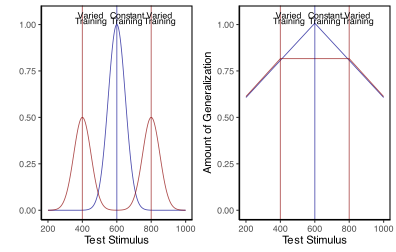
\includegraphics{full_files/figure-pdf/fig-toy-model1-1.pdf}

}

\caption{\label{fig-toy-model1}Left panel- Generalization predicted from
a simple model that assumes a linear generalization function. A varied
group (red vertical lines indicate the 2 training locations) trained
from positions 400 and 800, and a constant group (blue vertical line),
trained from position 600. Right panel- if a Gaussian generalization
function is assumed, then varied training (400, 800) is predicted to
result in better generalization to positions close to 400 and 800 than
does constant training at 600. (For interpretation of the references to
color in this figure legend, the reader is referred to the web version
of this article.)}

\end{figure}%

In addition to largely overlooking the potential for non-linear
generalization to confound interpretations of training manipulations,
the visuomotor skill learning literature also rarely considers
alternatives to schema representations
\autocite{chamberlinMemoryRepresentationMotor1992}. Although
schema-theory remains influential within certain literatures, instance
or exemplar-based models have accounted for human behavior across myriad
domains
\autocite{jamiesonInstanceTheoryDomaingeneral2022,loganInstanceTheoryAttention2002a}.
As mentioned above, instance based accounts have been shown to perform
well on a variety of different tasks with motoric components
\autocite{crumpEpisodicContributionsSequential2010,gandolfoMotorLearningField1996a,meighWhatMemoryRepresentation2018,rosenbaumPlanningReachesEvaluating1995,vandamMappingShapeVisuomotor2015}.
However, such accounts have received little attention within the
subdomain of visuomotor skill learning focused on the benefits of varied
training.

The present work examines whether the commonly observed benefits of
varied training can be accounted for by between-group differences in
similarity between training and testing throws. We first attempt to
replicate previous work finding an advantage of varied training over
constant training in a projectile launching task. We then examine the
extent to which this advantage can be explained by an instance-based
similarity model.

\section{Experiment 1}\label{experiment-1}

\subsection{Methods}\label{methods}

\subsubsection{Sample Size Estimation}\label{sample-size-estimation}

To obtain an independent estimate of effect size, we identified previous
investigations which included between-subjects contrasts of varied and
constant conditions following training on an accuracy based projectile
launching task
\autocite{chuaPracticeVariabilityPromotes2019,goodwinEffectDifferentQuantities1998,kerrSpecificVariedPractice1978,wulfEffectTypePractice1991}.
We then averaged effects across these studies, yielding a Cohens f =.43.
The GPower 3.1 software package
\autocite{faulStatisticalPowerAnalyses2009}, 2009) was then used to
determine that a power of 80\% requires a sample size of at least 23
participants per condition. All experiments reported in the present
manuscript exceed this minimum number of participants per condition.

\subsubsection{Participants}\label{participants}

Participants were recruited from an undergraduate population that is
63\% female and consists almost entirely of individuals aged 18-22
years. A total of 110 Indiana University psychology students
participated in Experiment 1. We subsequently excluded 34 participants
poor performance at one of the dependent measures of the task (2.5-3
standard deviations worse than the median subject at the task) or for
displaying a pattern of responses that was clearly indicative of a lack
of engagement with the task (e.g.~simply dropping the ball on each trial
rather than throwing it at the target), or for reporting that they
completed the experiment on a phone or tablet device, despite the
instructions not to use one of these devices. A total of 74 participants
were retained for the final analyses, 35 in the varied group and 39 in
the constant group.

\subsubsection{Task}\label{task}

The experimental task was programmed in JavaScript, using packages from
the Phaser physics engine (https://phaser.io) and the jsPsych library
(de Leeuw, 2015). The stimuli, presented on a black background,
consisted of a circular blue ball -- controlled by the participant via
the mouse or trackpad cursor; a rectangular green target; a red
rectangular barrier located between the ball and the target; and an
orange square within which the participant could control the ball before
releasing it in a throw towards the target. Because the task was
administered online, the absolute distance between stimuli could vary
depending on the size of the computer monitor being used, but the
relative distance between the stimuli was held constant. Likewise, the
distance between the center of the target, and the training and testing
locations was scaled such that relative distances were preserved
regardless of screen size. For the sake of brevity, subsequent mentions
of this relative distance between stimuli, or the position where the
ball landed in relation to the center of the target, will be referred to
simply as distance. Figure~\ref{fig-IGAS_Methods} displays the layout of
the task, as it would appear to a participant at the start of a trial,
with the ball appearing in the center of the orange square. Using a
mouse or trackpad, participants click down on the ball to take control
of the ball, connecting the movement of the ball to the movement of the
cursor. Participants can then ``wind up'' the ball by dragging it
(within the confines of the orange square) and then launch the ball by
releasing the cursor. If the ball does not land on the target,
participants are presented with feedback in red text at the top right of
the screen, on how many units away they were from the center of the
target. If the ball was thrown outside of the boundary of the screen
participants are given feedback as to how far away from the target
center the ball would have been if it had continued its trajectory. If
the ball strikes the barrier (from the side or by landing on top),
feedback is presented telling participants to avoid hitting the barrier.
If participants drag the ball outside of the orange square before
releasing it, the trial terminates, and they are reminded to release the
ball within the orange square. If the ball lands on the target, feedback
is presented in green text, confirming that the target was hit, and
presenting additional feedback on how many units away the ball was from
the exact center of the target.

\href{https://pcl.sitehost.iu.edu/tg/demos/igas_expt1_demo.html}{Link to
abbrevaited example of task}.

\begin{figure}

\centering{


\includegraphics{full_files/figure-pdf/fig-IGAS_Methods-1.pdf}

}

\caption{\label{fig-IGAS_Methods}The stimuli of the task consisted of a
blue ball, which the participants would launch at the green target,
while avoiding the red barrier. On each trial, the ball would appear in
the center of the orange square, with the position of the orange square
varying between experimental conditions. Participants were constrained
to release the ball within the square}

\end{figure}%

\subsection{Results}\label{results}

\subsection{Data Processing and Statistical
Packages}\label{data-processing-and-statistical-packages}

To prepare the data, we first removed trials that were not easily
interpretable as performance indicators in our task. Removed trials
included: 1) those in which participants dragged the ball outside of the
orange starting box without releasing it, 2) trials in which
participants clicked on the ball, and then immediately released it,
causing the ball to drop straight down, 3) outlier trials in which the
ball was thrown more than 2.5 standard deviations further than the
average throw (calculated separately for each throwing position), and 4)
trials in which the ball struck the barrier. The primary measure of
performance used in all analyses was the absolute distance away from the
center of the target. The absolute distance was calculated on every
trial, and then averaged within each subject to yield a single
performance score, for each position. A consistent pattern across
training and testing phases in both experiments was for participants to
perform worse from throwing positions further away from the target -- a
pattern which we refer to as the difficulty of the positions. However,
there were no interactions between throwing position and training
conditions, allowing us to collapse across positions in cases where
contrasts for specific positions were not of interest. All data
processing and statistical analyses were performed in R version 4.03 (R
Core Team, 2020). ANOVAs for group comparisons were performed using the
rstatix package (Kassambara, 2021)****.

\subsection{Training Phase}\label{training-phase}

Figure~\ref{fig-IGAS_Training1} below shows aggregate training
performance binned into three stages representing the beginning, middle,
and end of the training phase. Because the two conditions trained from
target distances that were not equally difficult, it was not possible to
directly compare performance between conditions in the training phase.
Our focus for the training data analysis was instead to establish that
participants did improve their performance over the course of training,
and to examine whether there was any interaction between training stage
and condition. Descriptive statistics for the intermittent testing phase
are provided in the supplementary materials.

We performed an ANOVA comparison with stage as a within-group factor and
condition as between-group factor. The analysis revealed a significant
effect of training stage F(2,142)=62.4, p\textless.001, \(\eta^{2}_G\) =
.17, such that performance improved over the course of training There
was no significant effect of condition F(1,71)=1.42, p=.24,
\(\eta^{2}_G\) = .02, and no significant interaction between condition
and training stage, F(2,142)=.10, p=.91, \(\eta^{2}_G\) \textless{} .01.

\begin{figure}

\centering{

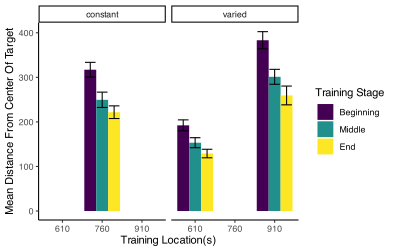
\includegraphics{full_files/figure-pdf/fig-IGAS_Training1-1.pdf}

}

\caption{\label{fig-IGAS_Training1}Training performance for varied and
constant participants binned into three stages. Shorter bars indicate
better performance (ball landing closer to the center of the target).
Error bars indicate standard error of the mean.}

\end{figure}%

\subsection{Testing Phase}\label{testing-phase}

In Experiment 1, a single constant-trained group was compared against a
single varied-trained group. At the transfer phase, all participants
were tested from 3 positions: 1) the positions(s) from their own
training, 2) the training position(s) of the other group, and 3) a
position novel to both groups. Overall, group performance was compared
with a mixed type III ANOVA, with condition (varied vs.~constant) as a
between-subject factor and throwing location as a within-subject
variable. The effect of throwing position was strong, F(3,213) = 56.12,
p\textless.001, η2G = .23. The effect of training condition was
significant F(1,71)=8.19, p\textless.01, η2G = .07. There was no
significant interaction between group and position, F(3,213)=1.81,
p=.15, η2G = .01.

\begin{figure}

\centering{

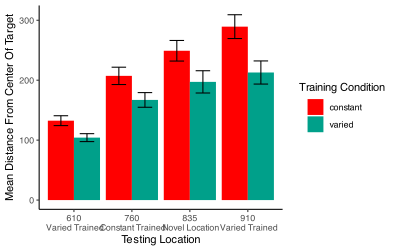
\includegraphics{full_files/figure-pdf/fig-IGAS_Testing1-1.pdf}

}

\caption{\label{fig-IGAS_Testing1}Testing performance for each of the 4
testing positions, compared between training conditions. Positions 610
and 910 were trained on by the varied group, and novel for the constant
group. Position 760 was trained on by the constant group, and novel for
the varied group. Position 835 was novel for both groups. Shorter bars
are indicative of better performance (the ball landing closer to the
center of the target). Error bars indicate standard error of the mean.}

\end{figure}%

\hfill\break
\hfill\break

\begin{table}

\caption{\label{tbl-IGAS_Table1}}

\centering{

\captionsetup{labelsep=none}

\begin{tabular}{lll}
\toprule
Position & Constant & Varied\\
\midrule
610 & 132.48(50.85) & 104.2(38.92)\\
760 & 207.26(89.19) & 167.12(72.29)\\
835 & 249.13(105.92) & 197.22(109.71)\\
910 & 289.36(122.48) & 212.86(113.93)\\
\bottomrule
\end{tabular}

}

\end{table}%

\subsection{Discussion}\label{discussion}

In Experiment 1, we found that varied training resulted in superior
testing performance than constant training, from both a position novel
to both groups, and from the position at which the constant group was
trained, which was novel to the varied condition. The superiority of
varied training over constant training even at the constant training
position is of particular note, given that testing at this position
should have been highly similar for participants in the constant
condition. It should also be noted, though, that testing at the constant
trained position is not exactly identical to training from that
position, given that the context of testing is different in several ways
from that of training, such as the testing trials from the different
positions being intermixed, as well as a simple change in context as a
function of time. Such contextual differences will be further considered
in the General Discussion.

In addition to the variation of throwing position during training, the
participants in the varied condition of Experiment 1 also received
training practice from the closest/easiest position, as well as from the
furthest/most difficult position that would later be encountered by all
participants during testing. The varied condition also had the potential
advantage of interpolating both of the novel positions from which they
would later be tested. Experiment 2 thus sought to address these issues
by comparing a varied condition to multiple constant conditions.

\section{Experiment 2}\label{experiment-2}

In Experiment 2, we sought to replicate our findings from Experiment 1
with a new sample of participants, while also addressing the possibility
of the pattern of results in Experiment 1 being explained by some
idiosyncrasy of the particular training location of the constant group
relative to the varied group. To this end, Experiment 2 employed the
same basic procedure as Experiment 1, but was designed with six separate
constant groups each trained from one of six different locations (400,
500, 625, 675, 800, or 900), and a varied group trained from two
locations (500 and 800). Participants in all seven groups were then
tested from each of the 6 unique positions.

\subsection{Methods}\label{methods-1}

\subsubsection{Participants}\label{participants-1}

A total of 306 Indiana University psychology students participated in
Experiment 2, which was also conducted online. As was the case in
experiment 1, the undergraduate population from which we recruited
participants was 63\% female and primarily composed of 18--22-year-old
individuals. Using the same procedure as experiment 1, we excluded 98
participants for exceptionally poor performance at one of the dependent
measures of the task, or for displaying a pattern of responses
indicative of a lack of engagement with the task. A total of 208
participants were included in the final analyses with 31 in the varied
group and 32, 28, 37, 25, 29, 26 participants in the constant groups
training from location 400, 500, 625, 675, 800, and 900, respectively.
All participants were compensated with course credit.

\subsubsection{Task and Procedure}\label{task-and-procedure}

The task of Experiment 2 was identical to that of Experiment 1, in all
but some minor adjustments to the height of the barrier, and the
relative distance between the barrier and the target. Additionally, the
intermittent testing trials featured in experiment 1 were not utilized
in experiment 2, and all training and testing trials were presented with
feedback. An abbreviated demo of the task used for Experiment 2 can be
found at (https://pcl.sitehost.iu.edu/tg/demos/igas\_expt2\_demo.html).

The procedure for Experiment 2 was also quite similar to experiment 1.
Participants completed 140 training trials, all of which were from the
same position for the constant groups and split evenly (70 trials each -
randomized) for the varied group. In the testing phase, participants
completed 30 trials from each of the six locations that had been used
separately across each of the constant groups during training. Each of
the constant groups thus experience one trained location and five novel
throwing locations in the testing phase, while the varied group
experiences 2 previously trained, and 4 novel locations.

\subsection{Results}\label{results-1}

\subsubsection{Data Processing and Statistical
Packages}\label{data-processing-and-statistical-packages-1}

After confirming that condition and throwing position did not have any
significant interactions, we standardized performance within each
position, and then average across position to yield a single performance
measure per participant. This standardization did not influence our
pattern of results. As in experiment 1, we performed type III ANOVA's
due to our unbalanced design, however the pattern of results presented
below is not altered if type 1 or type III tests are used instead. The
statistical software for the primary analyses was the same as for
experiment 1. Individual learning rates in the testing phase, compared
between groups in the supplementary analyses, were fit using the TEfit
package in R \autocite{cochraneTEfitsNonlinearRegression2020}.

\subsubsection{Training Phase}\label{training-phase-1}

The different training conditions trained from positions that were not
equivalently difficult and are thus not easily amenable to comparison.
As previously stated, the primary interest of the training data is
confirmation that some learning did occur. \textbf{?@fig-e2train}
depicts the training performance of the varied group alongside that of
the aggregate of the six constant groups (5a), and each of the 6
separate constant groups (5b). An ANOVA comparison with training stage
(beginning, middle, end) as a within-group factor and group (the varied
condition vs.~the 6 constant conditions collapsed together) as a
between-subject factor revealed no significant effect of group on
training performance, F(1,206)=.55,p=.49, \(\eta^{2}_G\) \textless.01, a
significant effect of training stage F(2,412)=77.91, p\textless.001,
\(\eta^{2}_G\) =.05, and no significant interaction between group and
training stage, F(2,412)=.489 p=.61, \(\eta^{2}_G\) \textless.01. We
also tested for a difference in training performance between the varied
group and the two constant groups that trained matching throwing
positions (i.e., the constant groups training from position 500, and
position 800). The results of our ANOVA on this limited dataset mirrors
that of the full-group analysis, with no significant effect of group
F(1,86)=.48, p=.49, \(\eta^{2}_G\) \textless.01, a significant effect of
training stage F(2,172)=56.29, p\textless.001, \(\eta^{2}_G\) =.11, and
no significant interaction between group and training stage,
F(2,172)=.341 p=.71, \(\eta^{2}_G\) \textless.01.

\begin{figure}

\centering{

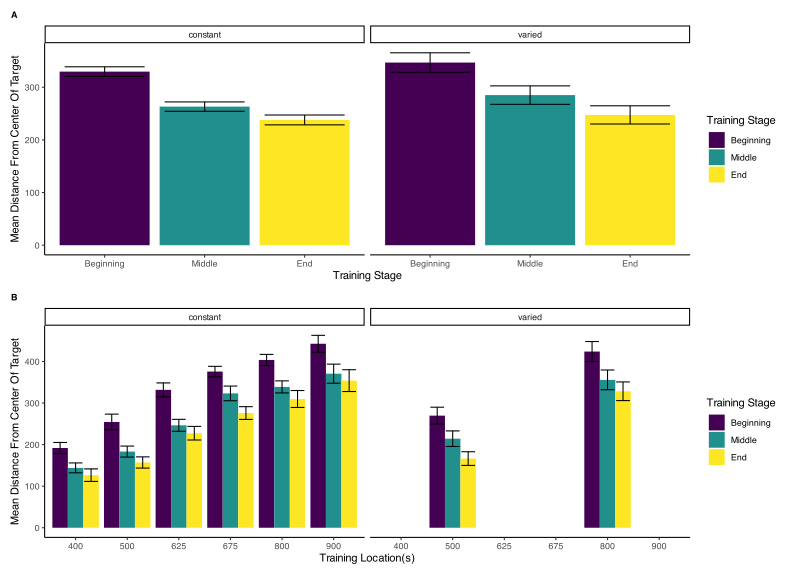
\includegraphics{full_files/figure-pdf/fig-e2train-1.pdf}

}

\caption{\label{fig-e2train-1}Training performance for the six constant
conditions, and the varied condition, binned into three stages. On the
left side, the six constant groups are averaged together, as are the two
training positions for the varied group. On the right side, the six
constant groups are shown separately, with each set of bars representing
the beginning, middle, and end of training for a single constant group
that trained from the position indicated on the x-axis. Figure 5b also
shows training performance separately for both of the throwing locations
trained by the varied group. Error bars indicate standard error of the
mean.}

\end{figure}%

\begin{figure}

\centering{

\includegraphics{full_files/figure-pdf/fig-e2train-2.pdf}

}

\caption{\label{fig-e2train-2}Training performance for the six constant
conditions, and the varied condition, binned into three stages. On the
left side, the six constant groups are averaged together, as are the two
training positions for the varied group. On the right side, the six
constant groups are shown separately, with each set of bars representing
the beginning, middle, and end of training for a single constant group
that trained from the position indicated on the x-axis. Figure 5b also
shows training performance separately for both of the throwing locations
trained by the varied group. Error bars indicate standard error of the
mean.}

\end{figure}%

\subsubsection{Testing Phase}\label{testing-phase-1}

In Experiment 2, a single varied condition (trained from two positions,
500 and 800), was compared against six separate constant groups (trained
from a single position, 400, 500, 625, 675, 800 or 900). For the testing
phase, all participants were tested from all six positions, four of
which were novel for the varied condition, and five of which were novel
for each of the constant groups. For a general comparison, we took the
absolute deviations for each throwing position and computed standardized
scores across all participants, and then averaged across throwing
position. The six constant groups were then collapsed together allowing
us to make a simple comparison between training conditions (constant vs.
varied). A type III between-subjects ANOVA was performed, yielding a
significant effect of condition F(1,206)=4.33, p=.039, \(\eta^{2}_G\)
=.02. Descriptive statistics for each condition are shown in table 2. In
Figure~\ref{fig-e2testa} visualizes the consistent advantage of the
varied condition over the constant groups across the testing positions.
Figure~\ref{fig-e2testa} shows performance between the varied condition
and the individual constant groups.

\begin{figure}

\centering{

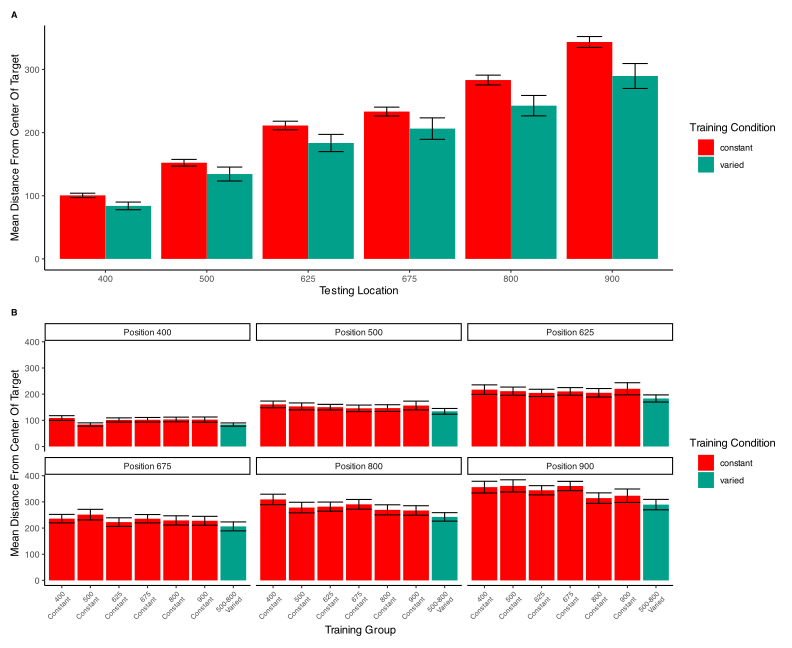
\includegraphics{full_files/figure-pdf/fig-e2testa-1.pdf}

}

\caption{\label{fig-e2testa}Testing phase performance from each of the
six testing positions. The six constant conditions are averaged together
into a single constant group, compared against the single varied-trained
group.B) Transfer performance from each of the 6 throwing locations from
which all participants were tested. Each bar represents performance from
one of seven distinct training groups (six constant groups in red, one
varied group in blue). The x axis labels indicate the location(s) from
which each group trained. Lower values along the y axis reflect better
performance at the task (closer distance to target center). Error bars
indicate standard error of the mean.}

\end{figure}%

\hfill\break
\hfill\break
\hfill\break

\begin{table}

\caption{\label{tbl-e2table1}Transfer performance from each of the 6
throwing locations from which all participants were tested. Each bar
represents performance from one of seven distinct training groups (six
constant groups in red, one varied group in blue). The x axis labels
indicate the location(s) from which each group trained. Lower values
along the y axis reflect better performance at the task (closer distance
to target center). Error bars indicate standard error of the mean.}

\centering{

\begin{tabular}{lll}
\toprule
Position & Constant & Varied\\
\midrule
400 & 100.59(46.3) & 83.92(33.76)\\
500 & 152.28(69.82) & 134.38(61.38)\\
625 & 211.21(90.95) & 183.51(75.92)\\
675 & 233.32(93.35) & 206.32(94.64)\\
800 & 283.24(102.85) & 242.65(89.73)\\
\addlinespace
900 & 343.51(114.33) & 289.62(110.07)\\
\bottomrule
\end{tabular}

}

\end{table}%

Next, we compared the testing performance of constant and varied groups
from only positions that participants had not encountered during
training. Constant participants each had 5 novel positions, whereas
varied participants tested from 4 novel positions (400,625,675,900). We
first standardized performance within in each position, and then
averaged across positions. Here again, we found a significant effect of
condition (constant vs.~varied): F(1,206)=4.30, p=.039, \(\eta^{2}_G\) =
.02 .

\begin{table}

\caption{\label{tbl-e2table2}Testing performance from novel positions.
Includes data only from positions that were not encountered during the
training stage (e.g.~excludes positions 500 and 800 for the varied
group, and one of the six locations for each of the constant groups).
Table presents Mean absolute deviations from the center of the target,
and standard deviations in parenthesis.}

\centering{

\begin{tabular}{lll}
\toprule
Position & Constant & Varied\\
\midrule
400 & 98.84(45.31) & 83.92(33.76)\\
500 & 152.12(69.94) & NA\\
625 & 212.91(92.76) & 183.51(75.92)\\
675 & 232.9(95.53) & 206.32(94.64)\\
800 & 285.91(102.81) & NA\\
\addlinespace
900 & 346.96(111.35) & 289.62(110.07)\\
\bottomrule
\end{tabular}

}

\end{table}%

Finally, corresponding to the comparison of position 760 from experiment
1, we compared the test performance of the varied group against the
constant group from only the positions that the constant groups trained.
Such positions were novel to the varied group (thus this analysis
omitted two constant groups that trained from positions 500 or 800 as
those positions were not novel to the varied group).
Figure~\ref{fig-e2test1} displays the particular subset of comparisons
utilized for this analysis. Again, we standardized performance within
each position before performing the analyses on the aggregated data. In
this case, the effect of condition did not reach statistical
significance F(1,149)=3.14, p=.079, \(\eta^{2}_G\) = .02. Table 4
provides descriptive statistics.

\begin{figure}

\centering{

\includegraphics{full_files/figure-pdf/fig-e2test1-1.pdf}

}

\caption{\label{fig-e2test1}A comparison of throwing location that are
identical to those trained by the constant participants (e.g.~constant
participants trained at position 900, tested from position 900), which
are also novel to the varied-trained participants (thus excluding
positions 500 and 800). Error bars indicate standard error of the mean.}

\end{figure}%

\hfill\break
\hfill\break

\begin{table}

\caption{\label{tbl-e2tab3}Testing performance from the locations
trained by constant participants and novel to varied participants.
Locations 500 and 800 are not included as these were trained by the
varied participants. Table presents Mean absolute deviation from the
center of the target, and standard deviations in parenthesis.}

\centering{

\begin{tabular}{lll}
\toprule
Position & Constant & Varied\\
\midrule
400 & 108.85(50.63) & 83.92(33.76)\\
625 & 204.75(84.66) & 183.51(75.92)\\
675 & 235.75(81.15) & 206.32(94.64)\\
900 & 323.5(130.9) & 289.62(110.07)\\
\bottomrule
\end{tabular}

}

\end{table}%

\subsection{Discussion}\label{discussion-1}

The results of experiment 2 largely conform to the findings of
experiment 1. Participants in both varied and constant conditions
improved at the task during the training phase. We did not observe the
common finding of training under varied conditions producing worse
performance during acquisition than training under constant conditions
\autocite{catalanoDistantTransferCoincident1984a,wrisbergVariabilityPracticeHypothesis1987},
which has been suggested to relate to the subsequent benefits of varied
training in retention and generalization testing
\autocite{soderstromLearningPerformanceIntegrative2015}. However our
finding of no difference in training performance between constant and
varied groups has been observed in previous work
\autocite{chuaPracticeVariabilityPromotes2019,moxleySchemaVariabilityPractice1979,pigottMotorSchemaStructure1984}.

In the testing phase, our varied group significantly outperformed the
constant conditions in both a general comparison, and in an analysis
limited to novel throwing positions. The observed benefit of varied over
constant training echoes the findings of many previous visuomotor skill
learning studies that have continued to emerge since the introduction of
Schmidt's influential Schema Theory
\autocite{catalanoDistantTransferCoincident1984a,chuaPracticeVariabilityPromotes2019,goodwinEffectDifferentQuantities1998,mccrackenTestSchemaTheory1977,moxleySchemaVariabilityPractice1979,newellVariabilityPracticeTransfer1976,pigottMotorSchemaStructure1984,rollerVariablePracticeLenses2001,schmidtSchemaTheoryDiscrete1975,willeyLongtermMotorLearning2018,wrisbergVariabilityPracticeHypothesis1987,wulfEffectTypePractice1991}.
We also join a much smaller set of research to observe this pattern in a
computerized task \autocite{seowTransferEffectsVaried2019}. One
departure from the experiment 1 findings concerns the pattern wherein
the varied group outperformed the constant group even from the training
position of the constant group, which was significant in experiment 1,
but did not reach significance in experiment 2. Although this pattern
has been observed elsewhere in the literature
\autocite{goodeSuperiorityVariableRepeated2008,kerrSpecificVariedPractice1978},
the overall evidence for this effect appears to be far weaker than for
the more general benefit of varied training in conditions novel to all
training groups.

\section{Computational Model}\label{computational-model}

Controlling for the similarity between training and testing The primary
goal of Experiment 2 was to examine whether the benefits of variability
would persist after accounting for individual differences in the
similarity between trained and tested throwing locations. To this end,
we modelled each throw as a two-dimensional point in the space of x and
y velocities applied to the projectile at the moment of release. For
each participant, we took each individual training throw, and computed
the similarity between that throw and the entire population of throws
within the solution space for each of the 6 testing positions. We
defined the solution space empirically as the set of all combinations of
x and y throw velocities that resulted in hitting the target. We then
summed each of the trial-level similarities to produce a single
similarity for each testing position score relating how the participant
threw the ball during training and the solutions that would result in
target hits from each of the six testing positions -- thus resulting in
six separate similarity scores for each participant.
Figure~\ref{fig-taskSpace} visualizes the solution space for each
location and illustrates how different combinations of x and y velocity
result in successfully striking the target from different launching
positions. As illustrated in Figure~\ref{fig-taskSpace}, the solution
throws represent just a small fraction of the entire space of velocity
combinations used by participants throughout the experiment.

\begin{figure}

\centering{

\includegraphics{full_files/figure-pdf/fig-taskSpace-1.pdf}

}

\caption{\label{fig-taskSpace}A) A visual representation of the
combinations of throw parameters (x and y velocities applied to the ball
at launch), which resulted in target hits during the testing phase. This
empirical solution space was compiled from all of the participants in
experiment 2. B) shows the solution space within the context of all of
the throws made throughout the testing phase of the experiment.}

\end{figure}%

For each individual trial, the Euclidean distance (Equation 1) was
computed between the velocity components (x and y) of that trial and the
velocity components of each individual solution throw for each of the 6
positions from which participants would be tested in the final phase of
the study. The P parameter in Equation 1 is set equal to 2, reflecting a
Gaussian similarity gradient. Then, as per an instance-based model of
similarity
\autocite{loganInstanceTheoryAttention2002a,nosofskySimilarityScalingCognitive1992},
these distances were multiplied by a sensitivity parameter, c, and then
exponentiated to yield a similarity value. The parameter c controls the
rate with which similarity-based generalization drops off as the
Euclidean distance between two throws in x- and y-velocity space
increases. If c has a large value, then even a small difference between
two throws' velocities greatly decreases the extent of generalization
from one to the other. A small value for c produces broad generalization
from one throw to another despite relatively large differences in their
velocities. The similarity values for each training individual throw
made by a given participant were then summed to yield a final similarity
score, with a separate score computed for each of the 6 testing
positions. The final similarity score is construable as index of how
accurate the throws a participant made during the training phase would
be for each of the testing positions.

\textbf{Equation 1:} \[ Similarity_{I,J} = \sum_{i=I}\sum_{j=J}
(e^{-c^\cdot d^{p}_{i,j}}) \]

\textbf{Equation 2:}
\[ d_{i,j} = \sqrt{(x_{Train_i}-x_{Solution_j})^2 + (y_{Train_i}-y_{Solution_j})^2 } \]

A simple linear regression revealed that these similarity scores were
significantly predictive of performance in the transfer stage, t
=-15.88, p\textless.01, \(r^2\)=.17, such that greater similarity
between training throws and solution spaces for each of the test
locations resulted in better performance. We then repeated the group
comparisons above while including similarity as a covariate in the
model. Comparing the varied and constant groups in testing performance
from all testing positions yielded a significant effect of similarity,
F(1, 205)=85.66, p\textless.001, \(\eta^{2}_G\) =.29, and also a
significant effect of condition (varied vs.~constant), F(1, 205)=6.03,
p=.015, \(\eta^{2}_G\) =.03. The group comparison limited to only novel
locations for the varied group pit against trained location for the
constant group resulted in a significant effect of similarity,
F(1,148)=31.12, p\textless.001, \(\eta^{2}_G\) =.18 as well as for
condition F(1,148)=11.55, p\textless.001, \(\eta^{2}_G\) =.07. For all
comparisons, the pattern of results was consistent with the initial
findings from experiment 2, with the varied group still performing
significantly better than the constant group.

\subsection{Fitting model parameters separately by
group}\label{fitting-model-parameters-separately-by-group}

To directly control for similarity in Experiment 2, we developed a
model-based measure of the similarity between training throws and
testing conditions. This similarity measure was a significant predictor
of testing performance, e.g., participants whose training throws were
more similar to throws that resulted in target hits from the testing
positions, tended to perform better during the testing phase.
Importantly, the similarity measure did not explain away the group-level
benefits of varied training, which remained significant in our linear
model predicting testing performance after similarity was added to the
model. However, previous research has suggested that participants may
differ in their level of generalization as a function of prior
experience, and that such differences in generalization gradients can be
captured by fitting the generalization parameter of an instance-based
model separately to each group
\autocite{hahnEffectsCategoryDiversity2005,lambertsFlexibleTuningSimilarity1994}.
Relatedly, the influential Bayesian generalization model developed by
\textcite{tenenbaumGeneralizationSimilarityBayesian2001a} predicts that
the breadth of generalization will increase when a rational agent
encounters a wider variety of examples. Following these leads, we assume
that in addition to learning the task itself, participants are also
adjusting how generalizable their experience should be. Varied versus
constant participants may be expected to learn to generalize their
experience to different degrees. To accommodate this difference, the
generalization parameter of the instance-based model (in the present
case, the c parameter) can be allowed to vary between the two groups to
reflect the tendency of learners to adaptively tune the extent of their
generalization. One specific hypothesis is that people adaptively set a
value of c to fit the variability of their training experience
\autocite{nosofskyExemplarbasedAccountsMultiplesystem2000,sakamotoTrackingVariabilityLearning2006}.
If one's training experience is relatively variable, as with the
variable training condition, then one might infer that future test
situations will also be variable, in which case a low value of c will
allow better generalization because generalization will drop off slowly
with training-to-testing distance. Conversely, if one's training
experience has little variability, as found in the constant training
conditions, then one might adopt a high value of c so that
generalization falls off rapidly away from the trained positions.

To address this possibility, we compared the original instance-based
model of similarity fit against a modified model which separately fits
the generalization parameter, c, to varied and constant participants. To
perform this parameter fitting, we used the optim function in R, and fit
the model to find the c value(s) that maximized the correlation between
similarity and testing performance.

Both models generate distinct similarity values between training and
testing locations. Much like the analyses in Experiment 2, these
similarity values are regressed against testing performance in models of
the form shown below. As was the case previously, testing performance is
defined as the mean absolute distance from the center of the target
(with a separate score for each participant, from each position).

Linear models 1 and 3 both show that similarity is a significant
predictor of testing performance (p\textless.01). Of greater interest is
the difference between linear model 2, in which similarity is computed
from a single c value fit from all participants (Similarity1c), with
linear model 4, which fits the c parameter separately between groups
(Similarity2c). In linear model 2, the effect of training group remains
significant when controlling for Similarity1c (p\textless.01), with the
varied group still performing significantly better. However, in linear
model 4 the addition of the Similarity2c predictor results in the effect
of training group becoming nonsignificant (p=.40), suggesting that the
effect of varied vs.~constant training is accounted for by the
Similarity2c predictor. Next, to further establish a difference between
the models, we performed nested model comparisons using ANOVA, to see if
the addition of the training group parameter led to a significant
improvement in model performance. In the first comparison, ANOVA(Linear
Model 1, Linear Model 2), the addition of the training group predictor
significantly improved the performance of the model (F=22.07,
p\textless.01). However, in the second model comparison, ANOVA (Linear
model 3, Linear Model 4) found no improvement in model performance with
the addition of the training group predictor (F=1.61, p=.20).

Finally, we sought to confirm that similarity values generated from the
adjusted Similarity2c model had more predictive power than those
generated from the original Similarity1c model. Using the BIC function
in R, we compared BIC values between linear model 1 (BIC=14604.00) and
linear model 3 (BIC = 14587.64). The lower BIC value of model 3 suggests
a modest advantage for predicting performance using a similarity measure
computed with two c values over similarity computed with a single c
value. When fit with separate c values, the best fitting c parameters
for the model consistently optimized such that the c value for the
varied group (c=.00008) was smaller in magnitude than the c value for
the constant group(c= .00011). Recall that similarity decreases as a
Gaussian function of distance (equation 1 above), and a smaller value of
c will result in a more gradual drop-off in similarity as the distance
between training throws and testing solutions increases.

In summary, our modeling suggests that an instance-based model which
assumes equivalent generalization gradients between constant and varied
trained participants is unable to account for the extent of benefits of
varied over constant training observed at testing. The evidence for this
in the comparative model fits is that when a varied/constant dummy-coded
variable for condition is explicitly added to the model, the variable
adds a significant contribution to the prediction of test performance,
with the variable condition yielding better performance than the
constant conditions. However, if the instance-based generalization model
is modified to assume that the training groups can differ in the
steepness of their generalization gradient, by incorporating a separate
generalization parameter for each group, then the instance-based model
can account for our experimental results without explicitly taking
training group into account. Henceforth this model will be referred to
as the Instance-based Generalization with Adaptive Similarity (IGAS)
model.

\section{General Discussion}\label{general-discussion}

Across two experiments, we found evidence in support of the benefits of
variability hypothesis in a simple, computerized projectile throwing
task. Generalization was observed in both constant and varied
participants, in that both groups tended to perform better at novel
positions in the testing phase than did participants who started with
those positions in the training phase. However, varied trained
participants consistently performed better than constant trained
participants, in terms of both the testing phase in general, and in a
comparison that only included untrained positions. We also found some
evidence for the less commonly observed pattern wherein varied-trained
participants outperform constant-trained participants even from
conditions identical to the constant group training
\autocite{goodeSuperiorityVariableRepeated2008,greenPracticeVariabilityTransfer1995a,kerrSpecificVariedPractice1978}.
In experiment 1 varied participants performed significantly better on
this identity comparison. In Experiment 2, the comparison was not
significant initially, but became significant after controlling for the
similarity measure that incorporates only a single value for the
steepness of similarity-based generalization (c). Furthermore, we showed
that the general pattern of results from Experiment 2 could be
parsimoniously accommodated by an instance-based similarity model, but
only with the assumption that constant and varied participants
generalize their training experience to different degrees. Our results
thus suggest that the benefits of variation cannot be explained by the
varied-trained participants simply covering a broader range of the task
space. Rather, the modeling suggests that varied participants also learn
to adaptively tune their generalization function such that throwing
locations generalize more broadly to one another than they do in the
constant condition. A learning system could end up adopting a higher c
value in the constant than variable training conditions by monitoring
the trial-by-trial variability of the training items. The c parameter
would be adapted downwards when adjacent training items are dissimilar
to each other and adapted upwards when adjacent training items are the
same. In this fashion, contextually appropriate c values could be
empirically learned. This learning procedure would capture the insight
that if a situation has a high amount variability, then the learner
should be predisposed toward thinking that subsequent test items will
also show considerable variability, in which case generalization
gradients should be broad, as is achieved by low values for c.

Also of interest is whether the IGAS model can predict the pattern of
results wherein the varied condition outperforms the constant condition
even from the position on which the constant condition trained. Although
our models were fit using all of the Experiment 2 training and testing
data, not just that of the identity comparisons, in
\textbf{?@fig-Toy\_Model2} we demonstrate how a simplified version of
the IGAS model could in principle produce such a pattern. In addition to
the assumption of differential generalization between varied and
constant conditions, our simplified model makes explicit an assumption
that is incorporated into the full IGAS model -- namely that even when
being tested from a position identical to that which was trained, there
are always some psychological contextual differences between training
and testing throws, resulting in a non-zero dissimilarity.

\begin{figure}

\centering{

\includegraphics{full_files/figure-pdf/fig-Toy-Model2-1.pdf}

}

\caption{\label{fig-Toy-Model2}A simple model depicting the necessity of
both of two separately fit generalization parameters, c, and a positive
distance between training and testing contexts, in order for an instance
model to predict a pattern of varied training from stimuli 400 and 800
outperforming constant training from position 600 at a test position of
600. For the top left panel, in which the generalization model assumes a
single c value (-.008) for both varied and constant conditions, and
identical contexts across training and testing, the equation which
generates the varied condition is - Amount of Generalization =
\(e^{(c\cdot|x-800|)} + e^{(c\cdot|x-400|)}\), whereas the constant
group generalization is generated from \(2\cdot e^{(c\cdot|x-600|)}\).
For the top right panel, the c constants in the original equations are
different for the 2 conditions, with \(c=-.002\) for the varied
condition, and \(c=-.008\) for the constant condition. The bottom two
panels are generated from identical equations to those immediately
above, except for the addition of extra distance (100 units) to reflect
the assumption of some change in context between training and testing
conditions. Thus, the generalization model for the varied condition in
the bottom-right panel is of the form - Amount of Generalization =
\(e^{(c_{varied}\cdot|x-800|)}+e^{(c_{varied}\cdot|x-400|)}\) .}

\end{figure}%

As mentioned above, the idea that learners flexibly adjust their
generalization gradient based on prior experience does have precedent in
the domains of category learning
\autocite{ahaConceptLearningFlexible1992,briscoeConceptualComplexityBias2011,hahnEffectsCategoryDiversity2005,lambertsFlexibleTuningSimilarity1994,opdebeeckRepresentationPerceivedShape2008},
and sensorimotor adaptation
\autocite{marongelliAdvantageFlexibleNeuronal2013,taylorContextdependentGeneralization2013,thoroughmanRapidReshapingHuman2005}.
\textcite{lambertsFlexibleTuningSimilarity1994} showed that a simple
manipulation of background knowledge during a categorization test
resulted in participants generalizing their training experience more or
less broadly, and moreover that such a pattern could be captured by
allowing the generalization parameter of an instance-based similarity
model to be fit separately between conditions. The flexible
generalization parameter has also successfully accounted for
generalization behavior in cases where participants have been trained on
categories that differ in their relative variability
\autocite{hahnEffectsCategoryDiversity2005,sakamotoTrackingVariabilityLearning2006}.
However, to the best of our knowledge, IGAS is the first instance-based
similarity model that has been put forward to account for the effect of
varied training in a visuomotor skill task. Although IGAS was inspired
by work in the domain of category learning, its success in a distinct
domain may not be surprising in light of the numerous prior observations
that at least certain aspects of learning and generalization may operate
under common principles across different tasks and domains
\autocite{censorCommonMechanismsHuman2012,hillsCentralExecutiveSearch2010,jamiesonInstanceTheoryDomaingeneral2022,lawSharedMechanismsPerceptual2010,roarkComparingPerceptualCategory2021,rosenbaumAcquisitionIntellectualPerceptualMotor2001,vigoLearningDifficultyVisual2018,wallIdentifyingRelationshipsCognitive2021,wuSimilaritiesDifferencesSpatial2020,yangGeneralLearningAbility2020}.

Our modelling approach does differ from category learning
implementations of instance-based models in several ways. One such
difference is the nature of the training instances that are assumed to
be stored. In category learning studies, instances are represented as
points in a multidimensional space of all of the attributes that define
a category item (e.g.~size/color/shape). Rather than defining instances
in terms of what stimuli learners experience, our approach assumes that
stored, motor instances reflect how they act, in terms of the velocity
applied to the ball on each throw. An advantage of many motor learning
tasks is the relative ease with which task execution variables can be
directly measured (e.g.~movement force, velocity, angle, posture) in
addition to the decision and response time measures that typically
exhaust the data generated from more classical cognitive tasks. Of
course, whether learners actually are storing each individual motor
instance is a fundamental question beyond the scope of the current work
-- though as described in the introduction there is some evidence in
support of this idea
\autocite{chamberlinNoteSchemaExemplar1992,crumpEpisodicContributionsSequential2010,hommelEventFilesEvidence1998,meighWhatMemoryRepresentation2018,poldrackRelationshipSkillLearning1999}.
A particularly noteworthy instance-based model of sensory-motor behavior
is the Knowledge II model of Rosenbaum and colleagues
\autocite{cohenWhereGraspsAre2004,rosenbaumPlanningReachesEvaluating1995}.
Knowledge II explicitly defines instances as postures (joint
combinations), and is thus far more detailed than IGAS in regards to the
contents of stored instances. Knowledge II also differs from IGAS in
that learning is accounted for by both the retrieval of stored postures,
and the generation of novel postures via the modification of retrieved
postures. A promising avenue for future research would be to combine the
adaptive similarity mechanism of IGAS with the novel instance generation
mechanisms of Knowledge II.

Our findings also have some conceptual overlap with an earlier study on
the effects of varied training in a coincident timing task
\autocite{catalanoDistantTransferCoincident1984a}. In this task,
participants observe a series of lamps lighting up consecutively, and
attempt to time a button press with the onset of the final lamp. The
design consisted of four separate constant groups, each training from a
single lighting velocity, and a single varied group training with all
four of the lighting velocities used by the individual constant groups.
Participants were then split into four separate testing conditions, each
of which were tested from a single novel lighting velocity of varying
distance from the training conditions. The result of primary interest
was that all participants performed worse as the distance between
training and testing velocity increased -- a typical generalization
decrement. However, varied participants showed less of a decrement than
did constant participants. The authors take this result as evidence that
varied training results in a less-steep generalization gradient than
does constant training. Although the experimental conclusions of
Catalano and Kleiner are similar to our own, our work is novel in that
we account for our results with a cognitive model, and without assuming
the formation of a schema. Additionally, the way in which Catalano and
Kleiner collapse their separate constant groups together may result in
similarity confounds between varied and constant conditions that leaves
their study open to methodological criticisms, especially in light of
related work which demonstrated that the extent to which varied training
may be beneficial can depend on whether the constant group they are
compared against trained from similar conditions to those later tested
\autocite{wrisbergVariabilityPracticeHypothesis1987}. Our study
alleviates such concerns by explicitly controlling for similarity.

\subsection{Limitations}\label{limitations}

A limitation of this study concerns the ordering of the testing/transfer
trials at the conclusion of both experiments. Participants were tested
from each separate position (4 in Experiment 1, 6 in Experiment 2) in a
random, intermixed order. Because the varied group was trained from two
positions that were also randomly ordered, they may have benefited from
experience with this type of sequencing, whereas the constant groups had
no experience with switching between positions trial to trial. This
concern is somewhat ameliorated by the fact that the testing phase
performance of the constant groups from their trained position was not
significantly worse than their level of performance at the end of the
training phase, suggesting that they were not harmed by random ordering
of positions during testing. It should also be noted that the
computerized task utilized in the present work is relatively simple
compared to many of the real-world tasks utilized in prior research. It
is thus conceivable that the effect of variability in more complex tasks
is distinct from the process put forward in the present work. An
important challenge for future work will be to assess the extent to
which IGAS can account for generalization in relatively complex tasks
with far more degrees of freedom.

It is common for psychological process models of categorization learning
to use an approach such as multidimensional scaling so as to transform
the stimuli from the physical dimensions used in the particular task
into the psychological dimensions more reflective of the actual human
representations
\autocite{nosofskySimilarityScalingCognitive1992,shepardUniversalLawGeneralization1987}.
Such scaling typically entails having participants rate the similarity
between individual items and using these similarity judgements to then
compute the psychological distances between stimuli, which can then be
fed into a subsequent model. In the present investigation, there was no
such way to scale the x and y velocity components in terms of the
psychological similarity, and thus our modelling does rely on the
assumption that the psychological distances between the different
throwing positions are proportional to absolute distances in the metric
space of the task (e.g. the relative distance between positions 400 and
500 is equivalent to that between 800 and 900). However, an advantage of
our approach is that we are measuring similarity in terms of how
participants behave (applying a velocity to the ball), rather than the
metric features of the task stimuli.

\subsection{Conclusion}\label{conclusion}

Our experiments demonstrate a reliable benefit of varied training in a
simple projectile launching task. Such results were accounted for by an
instance-based model that assumes that varied training results in the
computation of a broader similarity-based generalization gradient.
Instance-based models augmented with this assumption may be a valuable
approach towards better understanding skill generalization and transfer.

\section{Project 2}\label{project-2}

\begin{center}\rule{0.5\linewidth}{0.5pt}\end{center}

\href{https://tegorman13.github.io/htw/}{Link to HTW project page}\\

\href{https://tegorman13.github.io/htw/paper.html}{Working Draft of HTW
Manuscript}

\begin{center}\rule{0.5\linewidth}{0.5pt}\end{center}

\section{Introduction}\label{introduction-1}

A longstanding issue across both science and instruction has been to
understand how various aspects of an educational curriculum or training
program influence learning acquisition and generalization. One such
aspect, which has received a great deal of research attention, is the
variability of examples experienced during training
\autocite{ravivHowVariabilityShapes2022}. The influence of training
variation has been studied in numerous domains, including category
learning
\autocite{cohenCategoryVariabilityExemplar2001,posnerGenesisAbstractIdeas1968},
visuomotor learning \autocites{schmidtSchemaTheoryDiscrete1975}[
]{bernikerEffectsTrainingBreadth2014}, language learning
\autocite{perryLearnLocallyThink2010}, and education
\autocite{braithwaiteEffectsVariationPrior2015,guoEffectsExampleVariability2014}.
The pattern of results is complex, with numerous studies finding both
beneficial
\autocite{catalanoDistantTransferCoincident1984a,braunMotorTaskVariation2009,rollerVariablePracticeLenses2001},
as well as null or negative effects
\autocites{huHighvariabilityTrainingDoes2024,vanrossumSchmidtSchemaTheory1990}[
]{brekelmansDoesHighVariability2022}. The present study seeks to
contribute to the large body of existing research by examining the
influence of variability in visuomotor function learning - a domain in
which it has been relatively under-studied.

\subsection{Function Learning and
Extrapolation}\label{function-learning-and-extrapolation}

The study of human function learning investigates how people learn
relationships between continuous input and output values. Function
learning is studied both in tasks where individuals are exposed to a
sequence of input/output pairs
\autocite{deloshExtrapolationSineQua1997,mcdanielEffectsSpacedMassed2013},
or situations where observers are presented with a an incomplete
scatterplot or line graph and make predictions about regions of the plot
that don't contain data
\autocite{ciccioneCanHumansPerform2021a,courrieuQuickApproximationBivariate2012,saidExtrapolationAccuracyUnderestimates2021,schulzCommunicatingCompositionalPatterns2020}.

\textcite{carrollFunctionalLearningLearning1963} conducted the earliest
work on function learning. Input stimuli and output responses were both
lines of varying length. The correct output response was related to the
length of the input line by a linear, quadratic, or random function.
Participants in the linear and quadratic performed above chance levels
during extrapolation testing, with those in the linear condition
performing the best overall. Carroll argued that these results were best
explained by a ruled based model wherein learners form an abstract
representation of the underlying function. Subsequent work by
\textcite{brehmerHypothesesRelationsScaled1974},testing a wider array of
functional forms, provided further evidence for superior extrapolation
in tasks with linear functions. Brehmer argued that individuals start
out with an assumption of a linear function, but given sufficient error
will progressively test alternative hypothesis with polynomials of
greater degree. \textcite{kohFunctionLearningInduction1991} employed a
visuomotor function learning task, wherein participants were trained on
examples from an unknown function relating the length of an input line
to the duration of a response (time between keystrokes). In this domain,
participants performed best when the relation between line length and
response duration was determined by a power, as opposed to linear
function. Koh \& Meyer developed the log-polynomial adaptive-regression
model to account for their results.

The first significant challenge to the rule-based accounts of function
learning was put forth by \textcite{deloshExtrapolationSineQua1997} . In
their task, participants learned to associate stimulus magnitudes with
response magnitudes that were related via either linear, exponential, or
quadratic function. Participants approached ceiling performance by the
end of training in each function condition, and were able to correctly
respond in interpolation testing trials. All three conditions
demonstrated some capacity for extrapolation, however participants in
the linear condition tended to underestimate the true function, while
exponential and quadratic participants reliably overestimated the true
function on extrapolation trials. Extrapolation and interpolation
performance are depicted in Figure~\ref{fig-delosh-extrap}.

The authors evaluated both of the rule-based models introduced in
earlier research (with some modifications enabling trial-by-trial
learning). The polynomial hypothesis testing model
\autocite{carrollFunctionalLearningLearning1963,brehmerHypothesesRelationsScaled1974}
tended to mimic the true function closely in extrapolation, and thus
offered a poor account of the human data. The log-polynomial adaptive
regression model \autocite{kohFunctionLearningInduction1991} was able to
mimic some of the systematic deviations produced by human subjects, but
also predicted overestimation in cases where underestimation occurred.

The authors also introduced two new function-learning models. The
Associative Learning Model (ALM) and the extrapolation-association model
(EXAM). ALM is a two layer connectionist model adapted from the ALCOVE
model in the category learning literature
\autocite{kruschkeALCOVEExemplarbasedConnectionist1992}. ALM belongs to
the general class of radial-basis function neural networks, and can be
considered a similarity-based model in the sense that the nodes in the
input layer of the network are activated as a function of distance. The
EXAM model retains the same similarity based activation and associative
learning mechanisms as ALM, while being augmented with a linear rule
response mechanism. When presented with novel stimuli, EXAM will
retrieve the most similar input-output examples encountered during
training, and from those examples compute a local slope. ALM was able to
provide a good account of participant training and interpolation data in
all three function conditions, however it was unable to extrapolate.
EXAM, on the other hand, was able to reproduce both the extrapolation
underestimation, as well as the quadratic and exponential overestimation
patterns exhibited by the human participants. Subsequent research
identified some limitations in EXAM's ability to account for cases where
human participants learn and extrapolate sinusoidal function
\textcite{bottNonmonotonicExtrapolationFunction2004} or to scenarios
where different functions apply to different regions of the input space
\textcite{kalishPopulationLinearExperts2004}, though EXAM has been shown
to provide a good account of human learning and extrapolation in tasks
with bi-linear, V shaped input spaces
\textcite{mcdanielPredictingTransferPerformance2009}.

\subsubsection{Variability and Function
Learning}\label{variability-and-function-learning}

The influence of variability on function learning tasks has received
relatively little attention. The study by
\textcite{deloshExtrapolationSineQua1997} (described in detail above)
did include a variability manipulation (referred to as density in their
paper), wherein participants were trained with either either 8, 20, or
50 unique input-output pairs, with the total number of training trials
held constant. They found a minimal influence of variability on training
performance, and no difference between groups in interpolation or
extrapolation, with all three variability conditions displaying accurate
interpolation, and linearly biased extrapolation that was well accounted
for by the EXAM model.

In the domain of visuomotor learning,
\textcite{vandamMappingShapeVisuomotor2015} employed a task which
required participants to learn a linear function between the spikiness
of shape stimuli and the correct horizontal position to make a rapid
pointing response. The shapes ranged from very spiky to completely
circular at the extreme ends of the space. Participants trained with
intermediate shapes from a lower variation (2 shapes) or higher
variation (5 shapes) condition, with the 2 items of the lower varied
condition matching the items used on the extreme ends of the higher
variation training space. Learning was significantly slower in the
higher variation group. However, the two conditions did not differ when
tested with novel shapes, with both groups producing extrapolation
responses of comparable magnitudes to the most similar training item,
rather than in accordance with the true linear function. The authors
accounted for both learning and extrapolation performance with a
Bayesian learning model. Similar to ALM, the bayesian model assumes that
generalization occurs as a Gaussian function of the distance between
stimuli. However unlike ALM, the bayesian learning model utilizes more
elaborate probabilistic stimulus representations, with a separate Kalman
Filter for each shape stimulus.

\begin{figure}

\centering{

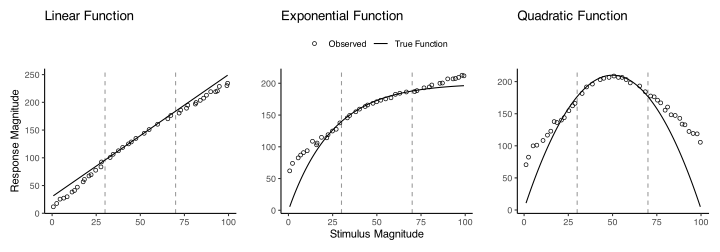
\includegraphics{full_files/figure-pdf/fig-delosh-extrap-1.pdf}

}

\caption{\label{fig-delosh-extrap}Generalization reproduced patterns
from DeLosh et al.~(1997) Figure 3. Stimulii that fall within the dashed
lines are interpolations of the training examples.}

\end{figure}%

\subsection{Overview Of Present Study}\label{overview-of-present-study}

The present study investigates the influence of training variability on
learning, generalization, and extrapolation in a uni-dimensional
visuomotor function learning task. To the best of our knowledge, this
research is the first to employ the classic constant vs.~varied training
manipulation, commonly used in the literature on the benefits of
variability, in the context of a uni-dimensional function learning task.
Across three experiments, we compare constant and varied training
conditions in terms of learning performance, extrapolation accuracy, and
the ability to reliably discriminate between stimuli.

To account for the empirical results, we will apply a series of
computational models, including the Associative Learning Model (ALM) and
the Extrapolation-Association Model (EXAM). Notably, this study is the
first to employ approximate Bayesian computation (ABC) to fit these
models to individual subject data, enabling us to thoroughly investigate
the full range of posterior predictions of each model, and to examine
the the ability of these influential models of function learning to
account for both the group level and individual level data.

\subsection{Methods}\label{methods-2}

\emph{Participants} A total of 156 participants were recruited from the
Indiana University Introductory Psychology Course. Participants were
randomly assigned to one of two training conditions: varied training or
constant training.

\emph{Task.} The ``Hit The Wall'' (HTW) visuomotor extrapolation task
task was programmed in Javascript, making heavy use of the
\href{https://phaser.io/}{phaser.io} game library. The HTW task involved
launching a projectile such that it would strike the ``wall'' at target
speed indicated at the top of the screen (see
Figure~\ref{fig-htw-task}). The target velocities were given as a range,
or band, of acceptable velocity values (e.g.~band 800-1000). During the
training stage, participants received feedback indicating whether they
had hit the wall within the target velocity band, or how many units
their throw was above or below from the target band. Participants were
instructed that only the x velocity component of the ball was relevant
to the task. The y velocity, or the location at which the ball struck
the wall, had no influence on the task feedback.

/

\begin{figure}

\centering{

\includegraphics[width=0.6\textwidth,height=\textheight]{../Assets/figs/htw_task_fig.png}

}

\caption{\label{fig-htw-task}The Hit the wall task. Participants launch
the blue ball to hit the red wall at the target velocity band indicated
at the top of the screen. The ball must be released from within the
orange square - but the location of release, and the location at which
the ball strikes the wall are both irrelevant to the task feedback.}

\end{figure}%

\emph{Procedure.} All participants completed the task online.
Participants were provided with a description of the experiment and
indicated informed consent. Figure~\ref{fig-design-e1} illustrates the
general procedure. Participants completed a total of 90 trials during
the training stage. In the varied training condition, participants
encountered three velocity bands (800-1000, 1000-1200, and 1200-1400).
Participants in the constant training condition trained on only one
velocity band (800-1000) - the closest band to what would be the novel
extrapolation bands in the testing stage.

Following the training stage, participants proceeded immediately to the
testing stage. Participants were tested from all six velocity bands, in
two separate stages. In the novel extrapolation testing stage,
participants completed ``no-feedback'' testing from three novel
extrapolation bands (100-300, 350-550, and 600-800), with each band
consisting of 15 trials. Participants were also tested from the three
velocity bands that were trained by the varied condition (800-1000,
1000-1200, and 1200-1400). In the constant training condition, two of
these bands were novel, while in the varied training condition, all
three bands were encountered during training. The order in which
participants completed the novel-extrapolation and testing-from-3-varied
bands was counterbalanced across participants. A final training stage
presented participants with ``feedback'' testing for each of the three
extrapolation bands (100-300, 350-550, and 600-800).

\begin{figure}

\centering{

\includegraphics[width=7in,height=2.5in]{full_files/figure-latex/dot-figure-1.png}

}

\caption{\label{fig-design-e1}Experiment 1 Design. Constant and Varied
participants complete different training conditions.}

\end{figure}%

\subsubsection{Analyses Strategy}\label{analyses-strategy}

All data processing and statistical analyses were performed in R version
4.32 \textcite{rcoreteamLanguageEnvironmentStatistical2020}. To assess
differences between groups, we used Bayesian Mixed Effects Regression.
Model fitting was performed with the brms package in R
\textcite{burknerBrmsPackageBayesian2017}, and descriptive stats and
tables were extracted with the BayestestR package
\textcite{makowskiBayestestRDescribingEffects2019}. Mixed effects
regression enables us to take advantage of partial pooling,
simultaneously estimating parameters at the individual and group level.
Our use of Bayesian, rather than frequentist methods allows us to
directly quantify the uncertainty in our parameter estimates, as well as
avoiding convergence issues common to the frequentist analogues of our
mixed models.

Each model was set to run with 4 chains, 5000 iterations per chain, with
the first 2500 discarded as warmup chains. Rhat values were within an
acceptable range, with values \textless=1.02 (see appendix for
diagnostic plots). We used uninformative priors for the fixed effects of
the model (condition and velocity band), and weakly informative Student
T distributions for for the random effects. For each model, we report 1)
the mean values of the posterior distribution for the parameters of
interest, 2) the lower and upper credible intervals (CrI), and the
probability of direction value (pd).

\begin{longtable}[]{@{}
  >{\raggedright\arraybackslash}p{(\columnwidth - 4\tabcolsep) * \real{0.2330}}
  >{\raggedright\arraybackslash}p{(\columnwidth - 4\tabcolsep) * \real{0.5728}}
  >{\raggedright\arraybackslash}p{(\columnwidth - 4\tabcolsep) * \real{0.1942}}@{}}
\toprule\noalign{}
\begin{minipage}[b]{\linewidth}\raggedright
Group Comparison
\end{minipage} & \begin{minipage}[b]{\linewidth}\raggedright
Code
\end{minipage} & \begin{minipage}[b]{\linewidth}\raggedright
Data
\end{minipage} \\
\midrule\noalign{}
\endhead
\bottomrule\noalign{}
\endlastfoot
End of Training Accuracy & \texttt{brm(dist\ \textasciitilde{}\ condit)}
& Final Training Block \\
Test Accuracy &
\texttt{brm(dist\ \textasciitilde{}\ condit\ *\ bandType\ +\ (1\textbar{}id)\ +\ (1\textbar{}bandInt)}
& All Testing trials \\
Band Discrimination &
\texttt{brm(vx\ \textasciitilde{}\ condit\ *\ band\ +(1\ +\ bandInt\textbar{}id)}
& All Testing Trials \\
\end{longtable}

\hfill\break

In each experiment we compare varied and constant conditions in terms of
1) accuracy in the final training block; 2) testing accuracy as a
function of band type (trained vs.~extrapolation bands); 3) extent of
discrimination between all six testing bands. We quantified accuracy as
the absolute deviation between the response velocity and the nearest
boundary of the target band. Thus, when the target band was velocity
600-800, throws of 400, 650, and 900 would result in deviation values of
200, 0, and 100, respectively. The degree of discrimination between
bands was index by fitting a linear model predicting the response
velocity as a function of the target velocity. Participants who reliably
discriminated between velocity bands tended to haves slope values
\textasciitilde1, while participants who made throws irrespective of the
current target band would have slopes \textasciitilde0.

\subsubsection{Results}\label{results-2}

\begin{figure}

\centering{

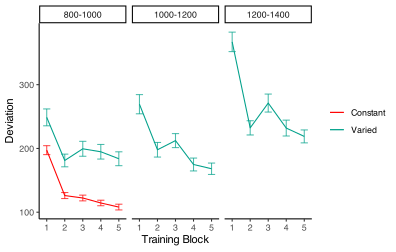
\includegraphics{full_files/figure-pdf/fig-e1-train-dev-1.pdf}

}

\caption{\label{fig-e1-train-dev}Experiment 1 Training Stage. Deviations
from target band across training blocks. Lower values represent greater
accuracy.}

\end{figure}%

\begin{longtable}[]{@{}lrrrr@{}}
\caption{\textbf{Experiment 1 - End of training performance}. The
Intercept represents the average of the baseline (constant condition),
and the conditVaried coefficient reflects the difference between the
constant and varied groups. A larger positive estimates indicates a
greater deviation (lower accuracy) for the varied
group.}\label{tbl-e1-train-dist}\tabularnewline
\toprule\noalign{}
Term & Estimate & 95\% CrI Lower & 95\% CrI Upper & pd \\
\midrule\noalign{}
\endfirsthead
\toprule\noalign{}
Term & Estimate & 95\% CrI Lower & 95\% CrI Upper & pd \\
\midrule\noalign{}
\endhead
\bottomrule\noalign{}
\endlastfoot
Intercept & 106.34 & 95.46 & 117.25 & 1 \\
conditVaried & 79.64 & 57.92 & 101.63 & 1 \\
\end{longtable}

\hfill\break

\emph{Training}. Figure~\ref{fig-e1-train-dev} displays the average
deviations across training blocks for the varied group, which trained on
three velocity bands, and the constant group, which trained on one
velocity band. To compare the training conditions at the end of
training, we analyzed performance on the 800-1000 velocity band, which
both groups trained on. The full model results are shown in Table 1. The
varied group had a significantly greater deviation than the constant
group in the final training block, (\(\beta\) = 79.64, 95\% CrI
{[}57.92, 101.63{]}; pd = 100\%).

\begin{longtable}[]{@{}
  >{\raggedright\arraybackslash}p{(\columnwidth - 8\tabcolsep) * \real{0.3425}}
  >{\raggedleft\arraybackslash}p{(\columnwidth - 8\tabcolsep) * \real{0.1644}}
  >{\raggedleft\arraybackslash}p{(\columnwidth - 8\tabcolsep) * \real{0.1644}}
  >{\raggedleft\arraybackslash}p{(\columnwidth - 8\tabcolsep) * \real{0.1644}}
  >{\raggedleft\arraybackslash}p{(\columnwidth - 8\tabcolsep) * \real{0.1644}}@{}}
\caption{\textbf{Experiment 1 testing accuracy}. Main effects of
condition and band type (training vs.~extrapolation), and the
interaction between the two factors. Larger coefficients indicate larger
deviations from the baselines (Condition=constant \& bandType=Trained) -
and a positive interaction coefficient indicates disproporionate
deviation for the varied condition on the extrapolation
bands}\label{tbl-e1-bmm-dist}\tabularnewline
\toprule\noalign{}
\begin{minipage}[b]{\linewidth}\raggedright
Term
\end{minipage} & \begin{minipage}[b]{\linewidth}\raggedleft
Estimate
\end{minipage} & \begin{minipage}[b]{\linewidth}\raggedleft
95\% CrI Lower
\end{minipage} & \begin{minipage}[b]{\linewidth}\raggedleft
95\% CrI Upper
\end{minipage} & \begin{minipage}[b]{\linewidth}\raggedleft
pd
\end{minipage} \\
\midrule\noalign{}
\endfirsthead
\toprule\noalign{}
\begin{minipage}[b]{\linewidth}\raggedright
Term
\end{minipage} & \begin{minipage}[b]{\linewidth}\raggedleft
Estimate
\end{minipage} & \begin{minipage}[b]{\linewidth}\raggedleft
95\% CrI Lower
\end{minipage} & \begin{minipage}[b]{\linewidth}\raggedleft
95\% CrI Upper
\end{minipage} & \begin{minipage}[b]{\linewidth}\raggedleft
pd
\end{minipage} \\
\midrule\noalign{}
\endhead
\bottomrule\noalign{}
\endlastfoot
Intercept & 152.55 & 70.63 & 229.85 & 1.0 \\
conditVaried & 39.00 & -21.10 & 100.81 & 0.9 \\
bandTypeExtrapolation & 71.51 & 33.24 & 109.60 & 1.0 \\
conditVaried:bandTypeExtrapolation & 66.46 & 32.76 & 99.36 & 1.0 \\
\end{longtable}

\emph{Testing.} To compare accuracy between groups in the testing stage,
we fit a Bayesian mixed effects model predicting deviation from the
target band as a function of training condition (varied vs.~constant)
and band type (trained vs.~extrapolation), with random intercepts for
participants and bands. The model results are shown in
Table~\ref{tbl-e1-bmm-dist}. The main effect of training condition was
not significant (\(\beta\) = 39, 95\% CrI {[}-21.1, 100.81{]}; pd =
89.93\%). The extrapolation testing items had a significantly greater
deviation than the training bands (\(\beta\) = 71.51, 95\% CrI {[}33.24,
109.6{]}; pd = 99.99\%). Most importantly, the interaction between
training condition and band type was significant (\(\beta\) = 66.46,
95\% CrI {[}32.76, 99.36{]}; pd = 99.99\%), As shown in
Figure~\ref{fig-e1-test-dev}, the varied group had disproportionately
larger deviations compared to the constant group in the extrapolation
bands.

\begin{figure}

\centering{

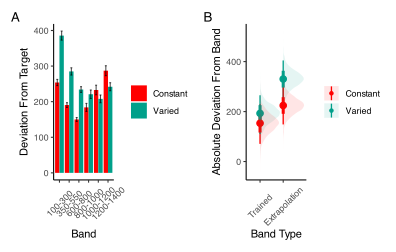
\includegraphics{full_files/figure-pdf/fig-e1-test-dev-1.pdf}

}

\caption{\label{fig-e1-test-dev}A) Deviations from target band during
testing without feedback stage. B) Conditional effect of condition
(Constant vs.~Varied) and testing band type (training vs.~extrapolation)
on testing accuracy. Error bars represent 95\% credible intervals.}

\end{figure}%

\hfill\break

\begin{longtable}[]{@{}lrrrr@{}}
\caption{Experiment 1. Bayesian Mixed Model Predicting velocity as a
function of condition (Constant vs.~Varied) and Velocity Band. Larger
coefficients on Band represent greater
sensitivity/discrimination.}\label{tbl-e1-bmm-vx}\tabularnewline
\toprule\noalign{}
Term & Estimate & 95\% CrI Lower & 95\% CrI Upper & pd \\
\midrule\noalign{}
\endfirsthead
\toprule\noalign{}
Term & Estimate & 95\% CrI Lower & 95\% CrI Upper & pd \\
\midrule\noalign{}
\endhead
\bottomrule\noalign{}
\endlastfoot
Intercept & 408.55 & 327.00 & 490.61 & 1.00 \\
conditVaried & 164.05 & 45.50 & 278.85 & 1.00 \\
Band & 0.71 & 0.62 & 0.80 & 1.00 \\
condit*Band & -0.14 & -0.26 & -0.01 & 0.98 \\
\end{longtable}

Finally, to assess the ability of both conditions to discriminate
between velocity bands, we fit a model predicting velocity as a function
of training condition and velocity band, with random intercepts and
random slopes for each participant. See Table~\ref{tbl-e1-bmm-vx} for
the full model results. The estimated coefficient for training condition
(\(\beta\) = 164.05, 95\% CrI {[}45.5, 278.85{]}, pd = 99.61\%) suggests
that the varied group tends to produce harder throws than the constant
group, but is not in and of itself useful for assessing discrimination.
Most relevant to the issue of discrimination is the coefficient on the
Band predictor (\(\beta\) = 0.71 95\% CrI {[}0.62, 0.8{]}, pd = 100\%).
Although the median slope does fall underneath the ideal of value of 1,
the fact that the 95\% credible interval does not contain 0 provides
strong evidence that participants exhibited some discrimination between
bands. The estimate for the interaction between slope and condition
(\(\beta\) = -0.14, 95\% CrI {[}-0.26, -0.01{]}, pd = 98.39\%), suggests
that the discrimination was somewhat modulated by training condition,
with the varied participants showing less sensitivity between bands than
the constant condition. This difference is depicted visually in
Figure~\ref{fig-e1-test-vx}.

\begin{figure}

\centering{

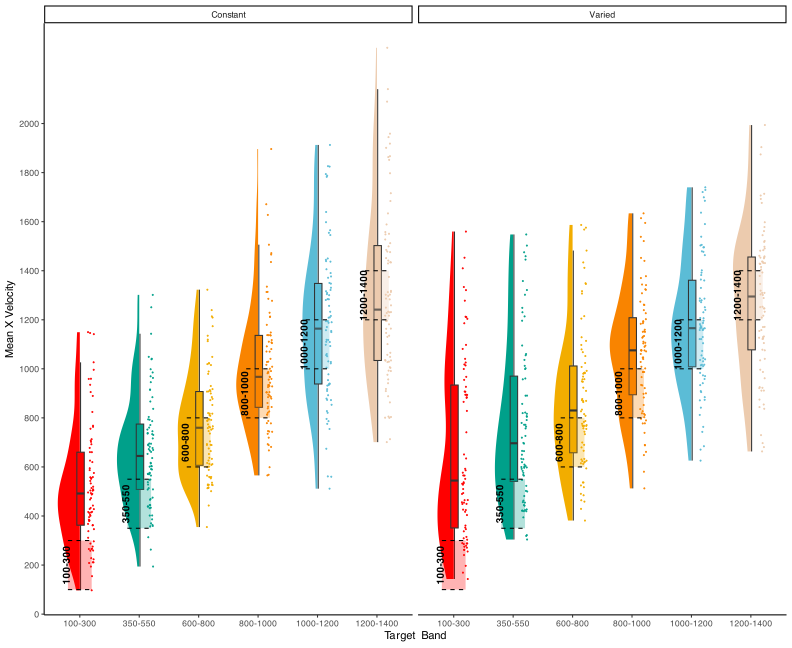
\includegraphics{full_files/figure-pdf/fig-e1-test-vx-1.pdf}

}

\caption{\label{fig-e1-test-vx}Empirical distribution of velocities
producing in testing stage. Translucent bands with dash lines indicate
the correct range for each velocity band.}

\end{figure}%

\begin{table}

\caption{\label{tbl-e1-bmm-vx}}

\centering{

\captionsetup{labelsep=none}

\begin{figure}[H]

{\centering 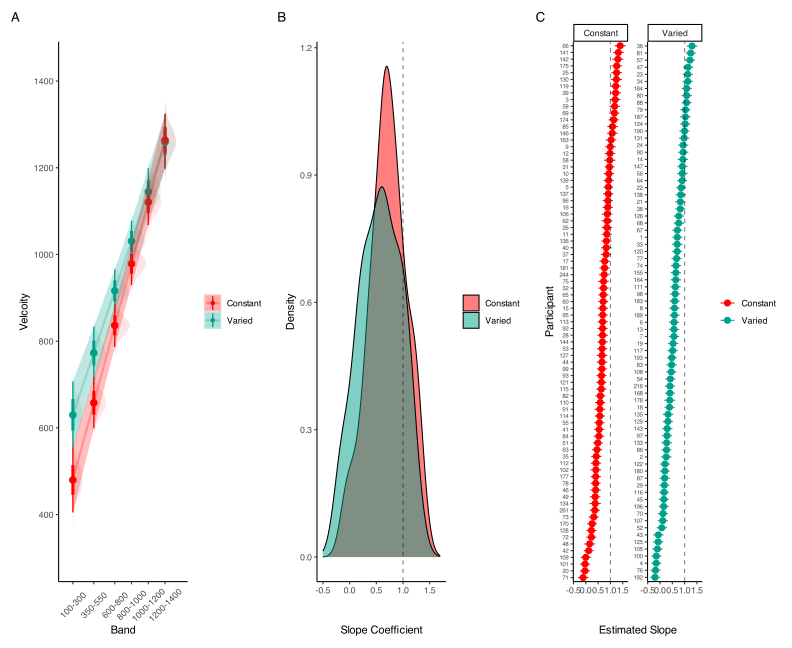
\includegraphics{full_files/figure-pdf/tbl-e1-bmm-vx-1.pdf}

}

\subcaption{Experiment 1. Conditional effect of training condition and
Band. Ribbons indicate 95\% HDI. The steepness of the lines serves as an
indicator of how well participants discriminated between velocity
bands.}

\end{figure}%

}

\end{table}%

\subsection{E1 Summary}\label{e1-summary}

In Experiment 1, we investigated how variability in training influenced
participants' ability learn and extrapolate in a visuomotor task. Our
findings that training with variable conditions rresulted in lower final
training performance is consistent with much of the prior researchon the
influence of training variability
\autocite{ravivHowVariabilityShapes2022,soderstromLearningPerformanceIntegrative2015},
and is particularly unsurprising in the present work, given that the
constant group received three times the amount of training on the
velocity band common to the two conditions.

More importantly, the varied training group exhibited significantly
larger deviations from the target velocity bands during the testing
phase, particularly for the extrapolation bands that were not
encountered by either condition during training.

\subsection{Experiment 2}\label{experiment-2-1}

\subsubsection{Methods \& Procedure}\label{methods-procedure}

The task and procedure of Experiment 2 was identical to Experiment 1,
with the exception that the training and testing bands were reversed
(see Figure~\ref{fig-design-e2}). The Varied group trained on bands
100-300, 350-550, 600-800, and the constant group trained on band
600-800. Both groups were tested from all six bands. A total of 110
participants completed the experiment (Varied: 55, Constant: 55).

\begin{figure}

\centering{

\includegraphics[width=8in,height=2.5in]{full_files/figure-latex/dot-figure-2.png}

}

\caption{\label{fig-design-e2}Experiment 2 Design. Constant and Varied
participants complete different training conditions. The training and
testing bands are the reverse of Experiment 1.}

\end{figure}%

\subsubsection{Results}\label{results-3}

\begin{figure}

\centering{

\includegraphics{full_files/figure-pdf/fig-e2-train-dev-1.pdf}

}

\caption{\label{fig-e2-train-dev}Experiment 2 Training Stage. Deviations
from target band across training blocks. Lower values represent greater
accuracy.}

\end{figure}%

\begin{longtable}[]{@{}lrrrr@{}}
\caption{\textbf{Experiment 2 - End of training performance}. The
Intercept represents the average of the baseline (constant condition),
and the conditVaried coefficient reflects the difference between the
constant and varied groups. A larger positive coefficient indicates a
greater deviation (lower accuracy) for the varied
group.}\label{tbl-e2-train-dist}\tabularnewline
\toprule\noalign{}
Term & Estimate & 95\% CrI Lower & 95\% CrI Upper & pd \\
\midrule\noalign{}
\endfirsthead
\toprule\noalign{}
Term & Estimate & 95\% CrI Lower & 95\% CrI Upper & pd \\
\midrule\noalign{}
\endhead
\bottomrule\noalign{}
\endlastfoot
Intercept & 91.01 & 80.67 & 101.26 & 1 \\
conditVaried & 36.15 & 16.35 & 55.67 & 1 \\
\end{longtable}

\hfill\break

\emph{Training}. Figure~\ref{fig-e2-train-dev} presents the deviations
across training blocks for both constant and varied training groups. We
again compared training performance on the band common to both groups
(600-800). The full model results are shown in Table 1. The varied group
had a significantly greater deviation than the constant group in the
final training block, ( \(\beta\) = 36.15, 95\% CrI {[}16.35, 55.67{]};
pd = 99.95\%).

\begin{longtable}[]{@{}
  >{\raggedright\arraybackslash}p{(\columnwidth - 8\tabcolsep) * \real{0.4390}}
  >{\raggedleft\arraybackslash}p{(\columnwidth - 8\tabcolsep) * \real{0.1220}}
  >{\raggedleft\arraybackslash}p{(\columnwidth - 8\tabcolsep) * \real{0.1829}}
  >{\raggedleft\arraybackslash}p{(\columnwidth - 8\tabcolsep) * \real{0.1829}}
  >{\raggedleft\arraybackslash}p{(\columnwidth - 8\tabcolsep) * \real{0.0732}}@{}}
\caption{\textbf{Experiment 2 testing accuracy}. Main effects of
condition and band type (training vs.~extrapolation), and the
interaction between the two factors. Larger coefficient estimates
indicate larger deviations from the baselines (constant \& trained
bands) - and a positive interaction coefficient indicates
disproporionate deviation for the varied condition on the extrapolation
bands}\label{tbl-e2-bmm-dist}\tabularnewline
\toprule\noalign{}
\begin{minipage}[b]{\linewidth}\raggedright
Term
\end{minipage} & \begin{minipage}[b]{\linewidth}\raggedleft
Estimate
\end{minipage} & \begin{minipage}[b]{\linewidth}\raggedleft
95\% CrI Lower
\end{minipage} & \begin{minipage}[b]{\linewidth}\raggedleft
95\% CrI Upper
\end{minipage} & \begin{minipage}[b]{\linewidth}\raggedleft
pd
\end{minipage} \\
\midrule\noalign{}
\endfirsthead
\toprule\noalign{}
\begin{minipage}[b]{\linewidth}\raggedright
Term
\end{minipage} & \begin{minipage}[b]{\linewidth}\raggedleft
Estimate
\end{minipage} & \begin{minipage}[b]{\linewidth}\raggedleft
95\% CrI Lower
\end{minipage} & \begin{minipage}[b]{\linewidth}\raggedleft
95\% CrI Upper
\end{minipage} & \begin{minipage}[b]{\linewidth}\raggedleft
pd
\end{minipage} \\
\midrule\noalign{}
\endhead
\bottomrule\noalign{}
\endlastfoot
Intercept & 190.91 & 125.03 & 259.31 & 1.00 \\
conditVaried & -20.58 & -72.94 & 33.08 & 0.78 \\
bandTypeExtrapolation & 38.09 & -6.94 & 83.63 & 0.95 \\
conditVaried:bandTypeExtrapolation & 82.00 & 41.89 & 121.31 & 1.00 \\
\end{longtable}

~\\

\emph{Testing Accuracy.} The analysis of testing accuracy examined
deviations from the target band as influenced by training condition
(Varied vs.~Constant) and band type (training vs.~extrapolation bands).
The results, summarized in Table~\ref{tbl-e2-bmm-dist}, reveal no
significant main effect of training condition (\(\beta\) = -20.58, 95\%
CrI {[}-72.94, 33.08{]}; pd = 77.81\%). However, the interaction between
training condition and band type was significant (\(\beta\) = 82, 95\%
CrI {[}41.89, 121.31{]}; pd = 100\%), with the varied group showing
disproportionately larger deviations compared to the constant group on
the extrapolation bands (see Figure~\ref{fig-e2-test-dev}).

\begin{figure}

\centering{

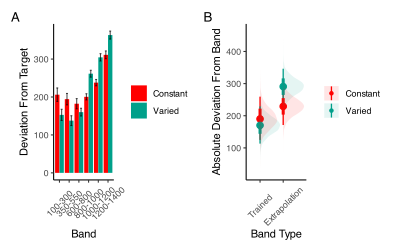
\includegraphics{full_files/figure-pdf/fig-e2-test-dev-1.pdf}

}

\caption{\label{fig-e2-test-dev}A) Deviations from target band during
testing without feedback stage. B) Estimated marginal means for the
interaction between training condition and band type. Error bars
represent 95\% confidence intervals.}

\end{figure}%

\begin{longtable}[]{@{}lrrrr@{}}
\caption{Experiment 2. Bayesian Mixed Model Predicting Vx as a function
of condition (Constant vs.~Varied) and Velocity
Band}\label{tbl-e2-bmm-vx}\tabularnewline
\toprule\noalign{}
Term & Estimate & 95\% CrI Lower & 95\% CrI Upper & pd \\
\midrule\noalign{}
\endfirsthead
\toprule\noalign{}
Term & Estimate & 95\% CrI Lower & 95\% CrI Upper & pd \\
\midrule\noalign{}
\endhead
\bottomrule\noalign{}
\endlastfoot
Intercept & 362.64 & 274.85 & 450.02 & 1.00 \\
conditVaried & -8.56 & -133.97 & 113.98 & 0.55 \\
Band & 0.71 & 0.58 & 0.84 & 1.00 \\
condit*Band & -0.06 & -0.24 & 0.13 & 0.73 \\
\end{longtable}

\emph{Testing Discrimination.} Finally, to assess the ability of both
conditions to discriminate between velocity bands, we fit a model
predicting velocity as a function of training condition and velocity
band, with random intercepts and random slopes for each participant. The
full model results are shown in Table~\ref{tbl-e2-bmm-vx}. The overall
slope on target velocity band predictor was significantly positive,
(\(\beta\) = 0.71, 95\% CrI {[}0.58, 0.84{]}; pd= 100\%), indicating
that participants exhibited discrimination between bands. The
interaction between slope and condition was not significant, (\(\beta\)
= -0.06, 95\% CrI {[}-0.24, 0.13{]}; pd= 72.67\%), suggesting that the
two conditions did not differ in their ability to discriminate between
bands (see Figure~\ref{fig-e2-test-vx}).

\begin{figure}

\centering{

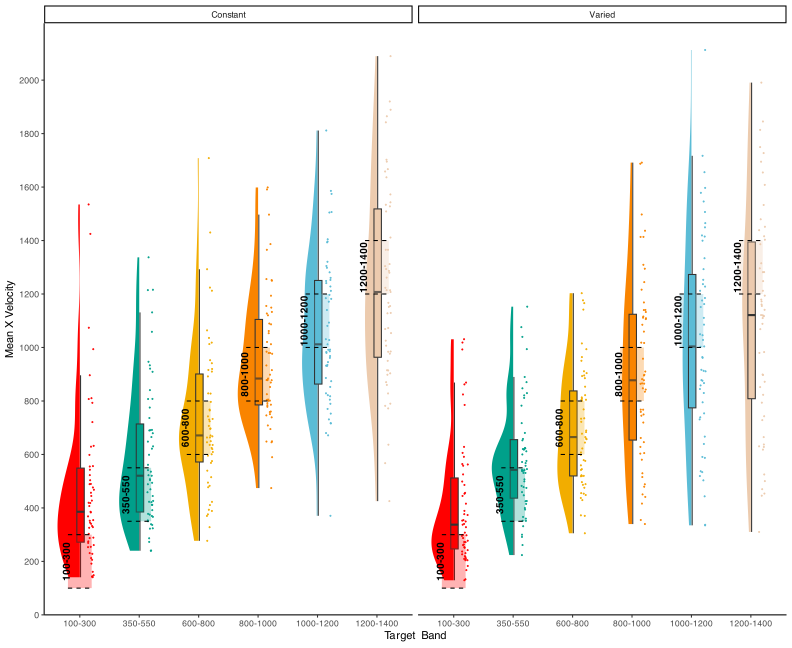
\includegraphics{full_files/figure-pdf/fig-e2-test-vx-1.pdf}

}

\caption{\label{fig-e2-test-vx}E2 testing x velocities. Translucent
bands with dash lines indicate the correct range for each velocity
band.}

\end{figure}%

\begin{table}

\caption{\label{tbl-e2-bmm-vx}}

\centering{

\captionsetup{labelsep=none}

\begin{figure}[H]

{\centering 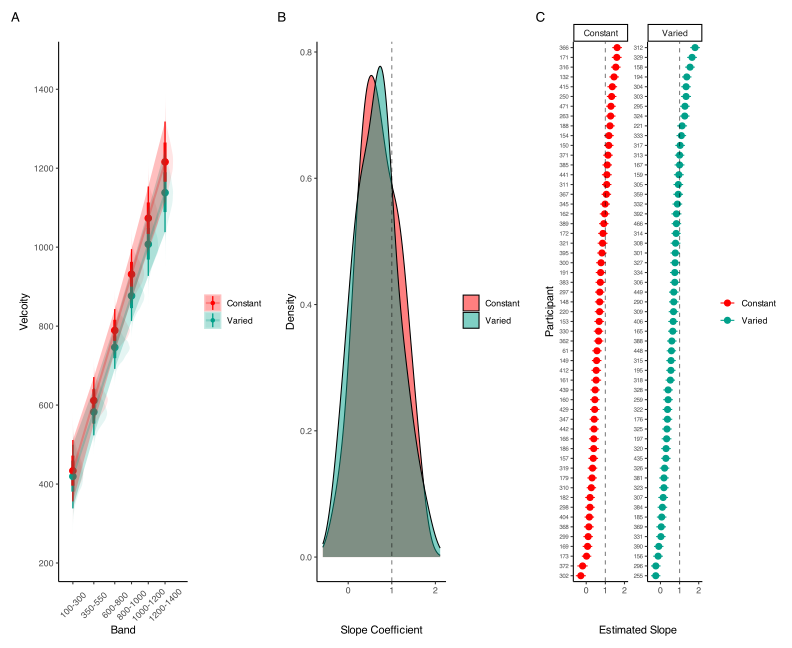
\includegraphics{full_files/figure-pdf/tbl-e2-bmm-vx-1.pdf}

}

\subcaption{Conditional effect of training condition and Band. Ribbons
indicate 95\% HDI. The steepness of the lines serves as an indicator of
how well participants discriminated between velocity bands.}

\end{figure}%

}

\end{table}%

\subsubsection{Experiment 2 Summary}\label{experiment-2-summary}

Experiment 2 extended the findings of Experiment 1 by examining the
effects of training variability on extrapolation performance in a
visuomotor function learning task, but with reversed training and
testing bands. Similar to Experiment 1, the Varied group exhibited
poorer performance during training and testing. However unlike
experiment 1, the Varied group did not show a significant difference in
discrimination between bands.

\subsection{Experiment 3}\label{experiment-3}

\subsubsection{Methods \& Procedure}\label{methods-procedure-1}

The major adjustment of Experiment 3 is for participants to receive
ordinal feedback during training, in contrast to the continuous feedback
of the prior experiments. After each training throw, participants are
informed whether a throw was too soft, too hard, or correct (i.e.~within
the target velocity range). All other aspects of the task and design are
identical to Experiments 1 and 2. We utilized the order of training and
testing bands from both of the prior experiments, thus assigning
participants to both an order condition (Original or Reverse) and a
training condition (Constant or Varied). Participants were once again
recruited from the online Indiana University Introductory Psychology
Course pool. Following exclusions, 195 participants were included in the
final analysis, n=51 in the Constant-Original condition, n=59 in the
Constant-Reverse condition, n=39 in the Varied-Original condition, and
n=46 in the Varied-Reverse condition.

\subsubsection{Results}\label{results-4}

\begin{longtable}[]{@{}
  >{\raggedright\arraybackslash}p{(\columnwidth - 8\tabcolsep) * \real{0.4026}}
  >{\raggedleft\arraybackslash}p{(\columnwidth - 8\tabcolsep) * \real{0.1299}}
  >{\raggedleft\arraybackslash}p{(\columnwidth - 8\tabcolsep) * \real{0.1948}}
  >{\raggedleft\arraybackslash}p{(\columnwidth - 8\tabcolsep) * \real{0.1948}}
  >{\raggedleft\arraybackslash}p{(\columnwidth - 8\tabcolsep) * \real{0.0779}}@{}}
\caption{\textbf{Experiment 3 - End of training performance}. The
Intercept represents the average of the baseline (constant condition),
and the conditVaried coefficient reflects the difference between the
constant and varied groups. A larger positive coefficient indicates a
greater deviation (lower accuracy) for the varied
group.}\label{tbl-e3-train-dist}\tabularnewline
\toprule\noalign{}
\begin{minipage}[b]{\linewidth}\raggedright
Term
\end{minipage} & \begin{minipage}[b]{\linewidth}\raggedleft
Estimate
\end{minipage} & \begin{minipage}[b]{\linewidth}\raggedleft
95\% CrI Lower
\end{minipage} & \begin{minipage}[b]{\linewidth}\raggedleft
95\% CrI Upper
\end{minipage} & \begin{minipage}[b]{\linewidth}\raggedleft
pd
\end{minipage} \\
\midrule\noalign{}
\endfirsthead
\toprule\noalign{}
\begin{minipage}[b]{\linewidth}\raggedright
Term
\end{minipage} & \begin{minipage}[b]{\linewidth}\raggedleft
Estimate
\end{minipage} & \begin{minipage}[b]{\linewidth}\raggedleft
95\% CrI Lower
\end{minipage} & \begin{minipage}[b]{\linewidth}\raggedleft
95\% CrI Upper
\end{minipage} & \begin{minipage}[b]{\linewidth}\raggedleft
pd
\end{minipage} \\
\midrule\noalign{}
\endhead
\bottomrule\noalign{}
\endlastfoot
Intercept & 121.86 & 109.24 & 134.60 & 1.00 \\
conditVaried & 64.93 & 36.99 & 90.80 & 1.00 \\
bandOrderReverse & 1.11 & -16.02 & 18.16 & 0.55 \\
conditVaried:bandOrderReverse & -77.02 & -114.16 & -39.61 & 1.00 \\
\end{longtable}

\emph{Training}. Figure~\ref{fig-e3-train-dev} displays the average
deviations from the target band across training blocks, and
Table~\ref{tbl-e3-train-dist} shows the results of the Bayesian
regression model predicting the deviation from the common band at the
end of training (600-800 for reversed order, and 800-1000 for original
order conditions). The main effect of training condition is significant,
with the varied condition showing larger deviations ( \(\beta\) = 64.93,
95\% CrI {[}36.99, 90.8{]}; pd = 100\%). The main effect of band order
is not significant \(\beta\) = 1.11, 95\% CrI {[}-16.02, 18.16{]}; pd =
55.4\%, however the interaction between training condition and band
order is significant, with the varied condition showing greater accuracy
in the reverse order condition ( \(\beta\) = -77.02, 95\% CrI
{[}-114.16, -39.61{]}; pd = 100\%).

\begin{figure}

\centering{

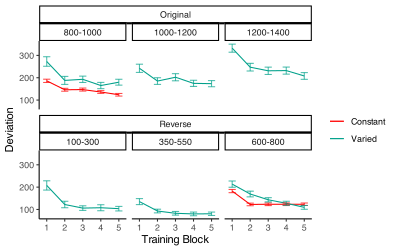
\includegraphics{full_files/figure-pdf/fig-e3-train-dev-1.pdf}

}

\caption{\label{fig-e3-train-dev}E3. Deviations from target band during
testing without feedback stage.}

\end{figure}%

\begin{longtable}[]{@{}
  >{\raggedright\arraybackslash}p{(\columnwidth - 8\tabcolsep) * \real{0.5354}}
  >{\raggedleft\arraybackslash}p{(\columnwidth - 8\tabcolsep) * \real{0.1010}}
  >{\raggedleft\arraybackslash}p{(\columnwidth - 8\tabcolsep) * \real{0.1515}}
  >{\raggedleft\arraybackslash}p{(\columnwidth - 8\tabcolsep) * \real{0.1515}}
  >{\raggedleft\arraybackslash}p{(\columnwidth - 8\tabcolsep) * \real{0.0606}}@{}}
\caption{\textbf{Experiment 3 testing accuracy}. Main effects of
condition and band type (training vs.~extrapolation), and the
interaction between the two factors. Larger coefficient estimates
indicate larger deviations from the baselines (constant training;
trained bands \& original order) - and a positive interaction
coefficient indicates disproportionate deviation for the varied
condition on the extrapolation
bands}\label{tbl-e3-bmm-dist}\tabularnewline
\toprule\noalign{}
\begin{minipage}[b]{\linewidth}\raggedright
Term
\end{minipage} & \begin{minipage}[b]{\linewidth}\raggedleft
Estimate
\end{minipage} & \begin{minipage}[b]{\linewidth}\raggedleft
95\% CrI Lower
\end{minipage} & \begin{minipage}[b]{\linewidth}\raggedleft
95\% CrI Upper
\end{minipage} & \begin{minipage}[b]{\linewidth}\raggedleft
pd
\end{minipage} \\
\midrule\noalign{}
\endfirsthead
\toprule\noalign{}
\begin{minipage}[b]{\linewidth}\raggedright
Term
\end{minipage} & \begin{minipage}[b]{\linewidth}\raggedleft
Estimate
\end{minipage} & \begin{minipage}[b]{\linewidth}\raggedleft
95\% CrI Lower
\end{minipage} & \begin{minipage}[b]{\linewidth}\raggedleft
95\% CrI Upper
\end{minipage} & \begin{minipage}[b]{\linewidth}\raggedleft
pd
\end{minipage} \\
\midrule\noalign{}
\endhead
\bottomrule\noalign{}
\endlastfoot
Intercept & 288.65 & 199.45 & 374.07 & 1.00 \\
conditVaried & -40.19 & -104.68 & 23.13 & 0.89 \\
bandTypeExtrapolation & -23.35 & -57.28 & 10.35 & 0.92 \\
bandOrderReverse & -73.72 & -136.69 & -11.07 & 0.99 \\
conditVaried:bandTypeExtrapolation & 52.66 & 14.16 & 90.23 & 1.00 \\
conditVaried:bandOrderReverse & -37.48 & -123.28 & 49.37 & 0.80 \\
bandTypeExtrapolation:bandOrderReverse & 80.69 & 30.01 & 130.93 &
1.00 \\
conditVaried:bandTypeExtrapolation:bandOrderReverse & 30.42 & -21.00 &
81.65 & 0.87 \\
\end{longtable}

\emph{Testing Accuracy.} Table~\ref{tbl-e3-bmm-dist} presents the
results of the Bayesian mixed efects model predicting absolute deviation
from the target band during the testing stage. There was no significant
main effect of training condition,\(\beta\) = -40.19, 95\% CrI
{[}-104.68, 23.13{]}; pd = 89.31\%, or band type,\(\beta\) = -23.35,
95\% CrI {[}-57.28, 10.35{]}; pd = 91.52\%. However the effect of band
order was significant, with the reverse order condition showing lower
deviations, \(\beta\) = -73.72, 95\% CrI {[}-136.69, -11.07{]}; pd =
98.89\%. The interaction between training condition and band type was
also significant \(\beta\) = 52.66, 95\% CrI {[}14.16, 90.23{]}; pd =
99.59\%, with the varied condition showing disproprionately large
deviations on the extrapolation bands compared to the constant group.
There was also a significant interaction between band type and band
order, \(\beta\) = 80.69, 95\% CrI {[}30.01, 130.93{]}; pd = 99.89\%,
such that the reverse order condition showed larger deviations on the
extrapolation bands. No other interactions were significant.

\begin{figure}

\centering{

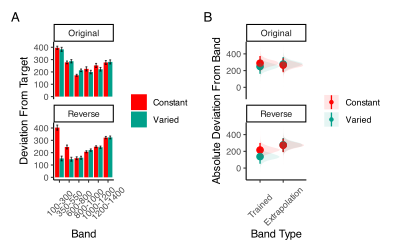
\includegraphics{full_files/figure-pdf/fig-e3-test-dev-1.pdf}

}

\caption{\label{fig-e3-test-dev}Experiment 3 Testing Accuracy. A)
Deviations from target band during testing without feedback stage. B)
Conditional effect of condition (Constant vs.~Varied) and testing band
type (training vs.~extrapolation) on testing accuracy. Error bars
represent 95\% confidence intervals.}

\end{figure}%

\begin{longtable}[]{@{}
  >{\raggedright\arraybackslash}p{(\columnwidth - 8\tabcolsep) * \real{0.4713}}
  >{\raggedleft\arraybackslash}p{(\columnwidth - 8\tabcolsep) * \real{0.1149}}
  >{\raggedleft\arraybackslash}p{(\columnwidth - 8\tabcolsep) * \real{0.1724}}
  >{\raggedleft\arraybackslash}p{(\columnwidth - 8\tabcolsep) * \real{0.1724}}
  >{\raggedleft\arraybackslash}p{(\columnwidth - 8\tabcolsep) * \real{0.0690}}@{}}
\caption{Experiment 3. Bayesian Mixed Model Predicting Vx as a function
of condition (Constant vs.~Varied) and Velocity
Band}\label{tbl-e3-bmm-vx}\tabularnewline
\toprule\noalign{}
\begin{minipage}[b]{\linewidth}\raggedright
Term
\end{minipage} & \begin{minipage}[b]{\linewidth}\raggedleft
Estimate
\end{minipage} & \begin{minipage}[b]{\linewidth}\raggedleft
95\% CrI Lower
\end{minipage} & \begin{minipage}[b]{\linewidth}\raggedleft
95\% CrI Upper
\end{minipage} & \begin{minipage}[b]{\linewidth}\raggedleft
pd
\end{minipage} \\
\midrule\noalign{}
\endfirsthead
\toprule\noalign{}
\begin{minipage}[b]{\linewidth}\raggedright
Term
\end{minipage} & \begin{minipage}[b]{\linewidth}\raggedleft
Estimate
\end{minipage} & \begin{minipage}[b]{\linewidth}\raggedleft
95\% CrI Lower
\end{minipage} & \begin{minipage}[b]{\linewidth}\raggedleft
95\% CrI Upper
\end{minipage} & \begin{minipage}[b]{\linewidth}\raggedleft
pd
\end{minipage} \\
\midrule\noalign{}
\endhead
\bottomrule\noalign{}
\endlastfoot
Intercept & 601.83 & 504.75 & 699.42 & 1.00 \\
conditVaried & 12.18 & -134.94 & 162.78 & 0.56 \\
bandOrderReverse & 13.03 & -123.89 & 144.67 & 0.58 \\
Band & 0.49 & 0.36 & 0.62 & 1.00 \\
conditVaried:bandOrderReverse & -338.15 & -541.44 & -132.58 & 1.00 \\
conditVaried:Band & -0.04 & -0.23 & 0.15 & 0.67 \\
bandOrderReverse:bandInt & -0.10 & -0.27 & 0.08 & 0.86 \\
conditVaried:bandOrderReverse:bandInt & 0.42 & 0.17 & 0.70 & 1.00 \\
\end{longtable}

\emph{Testing Discrimination.} The full results of the discrimination
model are presented in Table~\ref{tbl-e3-bmm-dist}. For the purposes of
assessing group differences in discrimination, only the coefficients
including the band variable are of interest. The baseline effect of band
represents the slope cofficient for the constant training - original
order condition, this effect was significant \(\beta\) = 0.49, 95\% CrI
{[}0.36, 0.62{]}; pd = 100\%. Neither of the two way interactions
reached significance, \(\beta\) = -0.04, 95\% CrI {[}-0.23, 0.15{]}; pd
= 66.63\%, \(\beta\) = -0.1, 95\% CrI {[}-0.27, 0.08{]}; pd = 86.35\%.
However, the three way interaction between training condition, band
order, and target band was significant, \(\beta\) = 0.42, 95\% CrI
{[}0.17, 0.7{]}; pd = 99.96\% - indicating that the varied condition
showed a greater slope coefficient on the reverse order bands, compared
to the constant condition - this is clearly shown in
Figure~\ref{fig-e3-test-vx}, where the steepness of the best fitting
line for the varied-reversed condition is noticably steeper than the
other conditions.

\begin{figure}

\centering{

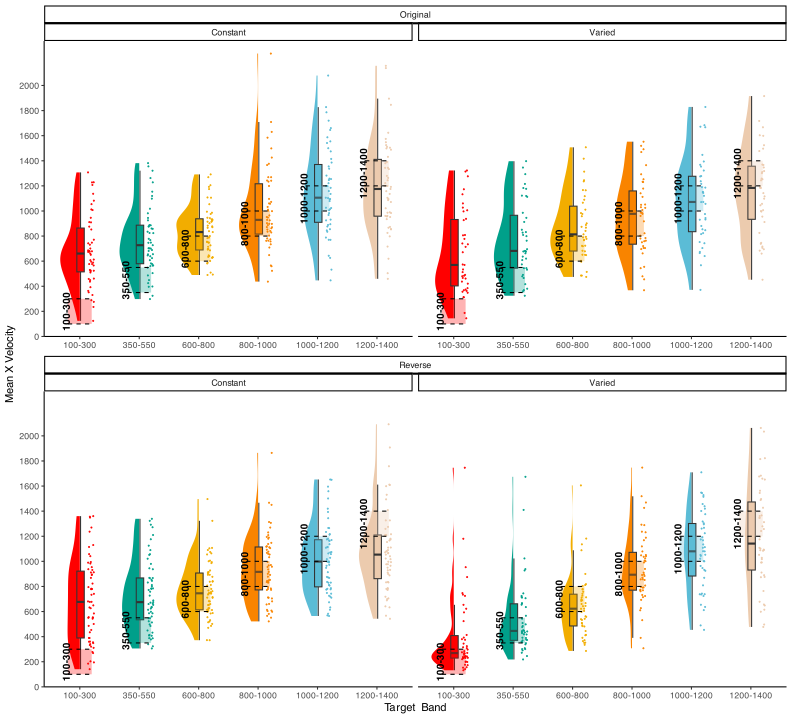
\includegraphics{full_files/figure-pdf/fig-e3-test-vx-1.pdf}

}

\caption{\label{fig-e3-test-vx}e3 testing x velocities. Translucent
bands with dash lines indicate the correct range for each velocity
band.}

\end{figure}%

\begin{figure}

\centering{

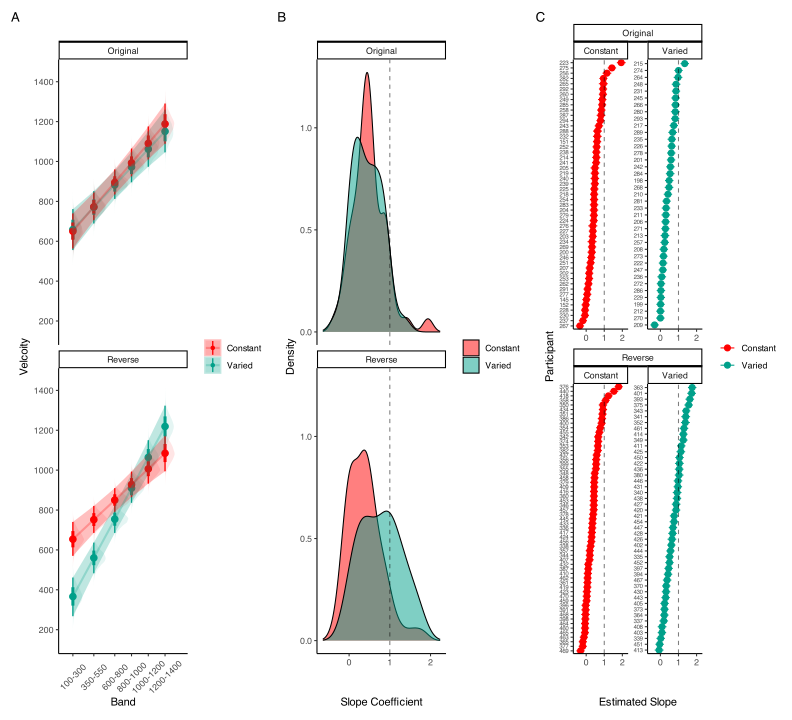
\includegraphics{full_files/figure-pdf/fig-e3-bmm-vx-1.pdf}

}

\caption{\label{fig-e3-bmm-vx}Conditional effect of training condition
and Band. Ribbons indicate 95\% HDI. The steepness of the lines serves
as an indicator of how well participants discriminated between velocity
bands.}

\end{figure}%

\subsubsection{Experiment 3 Summary}\label{experiment-3-summary}

\subsection{Computational Model}\label{computational-model-1}

\begin{figure}

\centering{

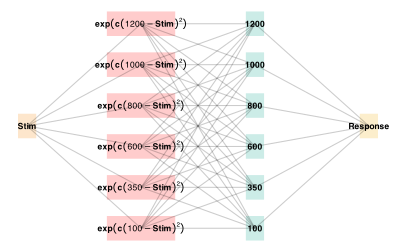
\includegraphics{full_files/figure-pdf/fig-alm-diagram-1.pdf}

}

\caption{\label{fig-alm-diagram}The Associative Learning Model (ALM).
The diagram illustrates the basic structure of the ALM model as used in
the present work. Input nodes are activated as a function of their
similarity to the lower-boundary of the target band. The generalization
parameter, \(c\), determines the degree to which nearby input nodes are
activated. The output nodes are activated as a function of the weighted
sum of the input nodes - weights are updated via the delta rule.}

\end{figure}%

\section{Modeling Approach}\label{modeling-approach}

The modeling goal is to implement a full process model capable of both
1) producing novel responses and 2) modeling behavior in both the
learning and testing stages of the experiment. For this purpose, we will
apply the associative learning model (ALM) and the EXAM model of
function learning \autocite{deloshExtrapolationSineQua1997}. ALM is a
simple connectionist learning model which closely resembles Kruschke's
ALCOVE model \autocite{kruschkeALCOVEExemplarbasedConnectionist1992},
with modifications to allow for the generation of continuous responses.

\subsection{ALM \& Exam Description}\label{alm-exam-description}

ALM is a localist neural network model
\autocite{pageConnectionistModellingPsychology2000a}, with each input
node corresponding to a particular stimulus, and each output node
corresponding to a particular response value. The units in the input
layer activate as a function of their Gaussian similarity to the input
stimulus. So, for example, an input stimulus of value 55 would induce
maximal activation of the input unit tuned to 55. Depending on the value
of the generalization parameter, the nearby units (e.g.~54 and 56; 53
and 57) may also activate to some degree. ALM is structured with input
and output nodes that correspond to regions of the stimulus space, and
response space, respectively. The units in the input layer activate as a
function of their similarity to a presented stimulus. As was the case
with the exemplar-based models, similarity in ALM is exponentially
decaying function of distance. The input layer is fully connected to the
output layer, and the activation for any particular output node is
simply the weighted sum of the connection weights between that node and
the input activations. The network then produces a response by taking
the weighted average of the output units (recall that each output unit
has a value corresponding to a particular response). During training,
the network receives feedback which activates each output unit as a
function of its distance from the ideal level of activation necessary to
produce the correct response. The connection weights between input and
output units are then updated via the standard delta learning rule,
where the magnitude of weight changes are controlled by a learning rate
parameter. The EXAM model is an extension of ALM, with the same learning
rule and representational scheme for input and output units. EXAM
differs from ALM only in its response rule, as it includes a linear
extrapolation mechanism for generating novel responses. Although this
extrapolation rule departs from a strictly similarity-based
generalization mechanism, EXAM is distinct from pure rule-based models
in that it remains constrained by the weights learned during training.
EXAM retrieves the two nearest training inputs, and the ALM responses
associated with those inputs, and computes the slope between these two
points. The slope is then used to extrapolate the response to the novel
test stimulus. Because EXAM requires at least two input-output pairs to
generate a response, additional assumptions were required in order for
it to generate resposnes for the constant group. We assumed that
participants come to the task with prior knowledge of the origin point
(0,0), which can serve as a reference point necessary for the model to
generate responses for the constant group. This assumption is motivated
by previous function learning research
(\textcite{brownUnderestimationLinearFunction2017}), which through a
series of manipulations of the y intercept of the underlying function,
found that participants consistently demonstrated knowledge of, or a
bias towards, the origin point (see
\textcite{kwantesWhyPeopleUnderestimate2006} for additional evidence of
such a bias in function learning tasks).

See Table~\ref{tbl-alm-exam} for a full specification of the equations
that define ALM and EXAM, and Figure~\ref{fig-alm-diagram} for a visual
representation of the ALM model.

\begin{figure*}

\begin{longtable}[]{@{}
  >{\raggedright\arraybackslash}p{(\columnwidth - 4\tabcolsep) * \real{0.2500}}
  >{\raggedright\arraybackslash}p{(\columnwidth - 4\tabcolsep) * \real{0.4028}}
  >{\raggedright\arraybackslash}p{(\columnwidth - 4\tabcolsep) * \real{0.3472}}@{}}
\caption{ALM \& EXAM Equations}\label{tbl-alm-exam}\tabularnewline
\toprule\noalign{}
\begin{minipage}[b]{\linewidth}\raggedright
\end{minipage} & \begin{minipage}[b]{\linewidth}\raggedright
\textbf{ALM Response Generation}
\end{minipage} & \begin{minipage}[b]{\linewidth}\raggedright
\end{minipage} \\
\midrule\noalign{}
\endfirsthead
\toprule\noalign{}
\begin{minipage}[b]{\linewidth}\raggedright
\end{minipage} & \begin{minipage}[b]{\linewidth}\raggedright
\textbf{ALM Response Generation}
\end{minipage} & \begin{minipage}[b]{\linewidth}\raggedright
\end{minipage} \\
\midrule\noalign{}
\endhead
\bottomrule\noalign{}
\endlastfoot
Input Activation &
\(a_i(X) = \frac{e^{-c(X-X_i)^2}}{\sum_{k=1}^M e^{-c(X-X_k)^2}}\) &
Input nodes activate as a function of Gaussian similarity to stimulus \\
Output Activation & \(O_j(X) = \sum_{k=1}^M w_{ji} \cdot a_i(X)\) &
Output unit \(O_j\) activation is the weighted sum of input activations
and association weights \\
Output Probability & \(P[Y_j|X] = \frac{O_j(X)}{\sum_{k=1}^M O_k(X)}\) &
The response, \(Y_j\) probabilites computed via Luce's choice rule \\
Mean Output &
\(m(X) = \sum_{j=1}^L Y_j \cdot \frac{O_j(x)}{\sum_{k=1}^M O_k(X)}\) &
Weighted average of probabilities determines response to X \\
& \textbf{ALM Learning} & \\
Feedback & \(f_j(Z) = e^{-c(Z-Y_j)^2}\) & feedback signal Z computed as
similarity between ideal response and observed response \\
magnitude of error & \(\Delta_{ji}=(f_{j}(Z)-o_{j}(X))a_{i}(X)\) & Delta
rule to update weights. \\
Update Weights & \(w_{ji}^{new}=w_{ji}+\eta\Delta_{ji}\) & Updates
scaled by learning rate parameter \(\eta\). \\
& \textbf{EXAM Extrapolation} & \\
Instance Retrieval & \(P[X_i|X] = \frac{a_i(X)}{\sum_{k=1}^M a_k(X)}\) &
Novel test stimulus \(X\) activates input nodes \(X_i\) \\
Slope Computation & \(S =\) \(\frac{m(X_{1})-m(X_{2})}{X_{1}-X_{2}}\) &
Slope value, \(S\) computed from nearest training instances \\
Response & \(E[Y|X_i] = m(X_i) + S \cdot [X - X_i]\) & ALM response
\(m(X_i)\) adjusted by slope. \\
\end{longtable}

\end{figure*}%

\subsection{Model Fitting}\label{model-fitting}

To fit ALM and EXAM to our participant data, we employ a similar method
to \textcite{mcdanielPredictingTransferPerformance2009}, wherein we
examine the performance of each model after being fit to various subsets
of the data. Each model was fit to the data in with separate procedures:
1) fit to maximize predictions of the testing data, 2) fit to maximize
predictions of both the training and testing data, 3) fit to maximize
predictions of the just the training data. We refer to this fitting
manipulations as ``Fit Method'' in the tables and figures below. It
should be emphasized that for all three fit methods, the ALM and EXAM
models behave identically - with weights updating only during the
training phase.Models to were fit separately to the data of each
individual participant. The free parameters for both models are the
generalization (\(c\)) and learning rate (\(lr\)) parameters. Parameter
estimation was performed using approximate bayesian computation (ABC),
which we describe in detail below.

\begin{tcolorbox}[enhanced jigsaw, toprule=.15mm, leftrule=.75mm, colframe=quarto-callout-color-frame, colback=white, left=2mm, breakable, bottomrule=.15mm, arc=.35mm, opacityback=0, rightrule=.15mm]

\textbf{\faIcon{lightbulb} Approximate Bayesian Computation}

To estimate the parameters of ALM and EXAM, we used approximate bayesian
computation (ABC), enabling us to obtain an estimate of the posterior
distribution of the generalization and learning rate parameters for each
individual. ABC belongs to the class of simulation-based inference
methods \autocite{cranmerFrontierSimulationbasedInference2020}, which
have begun being used for parameter estimation in cognitive modeling
relatively recently
\autocite{turnerTutorialApproximateBayesian2012,turnerBayesianAnalysisSimulationbased2016,kangasraasioParameterInferenceComputational2019}.
Although they can be applied to any model from which data can be
simulated, ABC methods are most useful for complex models that lack an
explicit likelihood function (e.g.~many neural network models).

The general ABC procedure is to 1) define a prior distribution over
model parameters. 2) sample candidate parameter values, \(\theta^*\),
from the prior. 3) Use \(\theta^*\) to generate a simulated dataset,
\(Data_{sim}\). 4) Compute a measure of discrepancy between the
simulated and observed datasets, \(discrep\)(\(Data_{sim}\),
\(Data_{obs}\)). 5) Accept \(\theta^*\) if the discrepancy is less than
the tolerance threshold, \(\epsilon\), otherwise reject \(\theta^*\). 6)
Repeat until desired number of posterior samples are obtained.

Although simple in the abstract, implementations of ABC require
researchers to make a number of non-trivial decisions as to i) the
discrepancy function between observed and simulated data, ii) whether to
compute the discrepancy between trial level data, or a summary statistic
of the datasets, iii) the value of the minimum tolerance \(\epsilon\)
between simulated and observed data. For the present work, we follow the
guidelines from previously published ABC tutorials
\autocite{turnerTutorialApproximateBayesian2012,farrellComputationalModelingCognition2018}.
For the test stage, we summarized datasets with mean velocity of each
band in the observed dataset as \(V_{obs}^{(k)}\) and in the simulated
dataset as \(V_{sim}^{(k)}\), where \(k\) represents each of the six
velocity bands. For computing the discrepancy between datasets in the
training stage, we aggregated training trials into three equally sized
blocks (separately for each velocity band in the case of the varied
group). After obtaining the summary statistics of the simulated and
observed datasets, the discrepancy was computed as the mean of the
absolute difference between simulated and observed datasets
(Equation~\ref{eq-discrep-test} and Equation~\ref{eq-discrep-train}).
For the models fit to both training and testing data, discrepancies were
computed for both stages, and then averaged together.

\begin{equation}\phantomsection\label{eq-discrep-test}{
discrep_{Test}(Data_{sim}, Data_{obs}) = \frac{1}{6} \sum_{k=1}^{6} |V_{obs}^{(k)} - V_{sim}^{(k)}|
}\end{equation}

\begin{equation}\phantomsection\label{eq-discrep-train}{
\begin{aligned} \\
discrep_{Train,constant}(Data_{sim}, Data_{obs}) = \frac{1}{N_{blocks}} \sum_{j=1}^{N_{blocks}} |V_{obs,constant}^{(j)} - V_{sim,constant}^{(j)}| \\ \\
discrep_{Train,varied}(Data_{sim}, Data_{obs}) = \frac{1}{N_{blocks} \times 3} \sum_{j=1}^{N_{blocks}} \sum_{k=1}^{3} |V_{obs,varied}^{(j,k)} - V_{sim,varied}^{(j,k)}|
\end{aligned}
}\end{equation}

The final component of our ABC implementation is the determination of an
appropriate value of \(\epsilon\). The setting of \(\epsilon\) exerts
strong influence on the approximated posterior distribution. Smaller
values of \(\epsilon\) increase the rejection rate, and improve the
fidelity of the approximated posterior, while larger values result in an
ABC sampler that simply reproduces the prior distribution. Because the
individual participants in our dataset differed substantially in terms
of the noisiness of their data, we employed an adaptive tolerance
setting strategy to tailor \(\epsilon\) to each individual. The initial
value of \(\epsilon\) was set to the overall standard deviation of each
individuals velocity values. Thus, sampled parameter values that
generated simulated data within a standard deviation of the observed
data were accepted, while worse performing parameters were rejected.
After every 300 samples the tolerance was allowed to increase only if
the current acceptance rate of the algorithm was less than 1\%. In such
cases, the tolerance was shifted towards the average discrepancy of the
5 best samples obtained thus far. To ensure the acceptance rate did not
become overly permissive, \(\epsilon\) was also allowed to decrease
every time a sample was accepted into the posterior.

\end{tcolorbox}

For each of the 156 participants from Experiment 1, the ABC algorithm
was run until 200 samples of parameters were accepted into the posterior
distribution. Obtaining this number of posterior samples required an
average of 205,000 simulation runs per participant. Fitting each
combination of participant, Model (EXAM \& ALM), and fitting method
(Test only, Train only, Test \& Train) required a total of 192 million
simulation runs. To facilitate these intensive computational demands, we
used the Future Package in R
\autocite{bengtssonUnifyingFrameworkParallel2021}, allowing us to
parallelize computations across a cluster of ten M1 iMacs, each with 8
cores.

\subsubsection{Modelling Results}\label{modelling-results}

\paragraph{Group level Patterns}\label{group-level-patterns}

\begin{longtable}{lcrrrr}

\caption{\label{tbl-htw-modelError-e1}Models errors predicting empirical
data - aggregated over all participants, posterior parameter values, and
velocity bands. Note that Fit Method refers to the subset of the data
that the model was trained on, while Task Stage refers to the subset of
the data that the model was evaluated on.}

\tabularnewline

\toprule
 &  & \multicolumn{2}{c}{ALM} & \multicolumn{2}{c}{EXAM} \\ 
\cmidrule(lr){3-4} \cmidrule(lr){5-6}
Task Stage & Fit Method & Constant & Varied & Constant & Varied \\ 
\midrule\addlinespace[2.5pt]
\cellcolor[HTML]{FFFFFF}{Test} & \cellcolor[HTML]{FFFFFF}{Fit to Test Data} & \cellcolor[HTML]{FFFFFF}{$199.93$} & \cellcolor[HTML]{FFFFFF}{$103.36$} & \cellcolor[HTML]{FFFFFF}{$104.01$} & \cellcolor[HTML]{FFFFFF}{$85.68$} \\ 
\cellcolor[HTML]{FFFFFF}{Test} & \cellcolor[HTML]{FFFFFF}{Fit to Test \& Training Data} & \cellcolor[HTML]{FFFFFF}{$216.97$} & \cellcolor[HTML]{FFFFFF}{$170.28$} & \cellcolor[HTML]{FFFFFF}{$127.94$} & \cellcolor[HTML]{FFFFFF}{$144.86$} \\ 
\cellcolor[HTML]{FFFFFF}{Test} & \cellcolor[HTML]{FFFFFF}{Fit to Training Data} & \cellcolor[HTML]{FFFFFF}{$467.73$} & \cellcolor[HTML]{FFFFFF}{$291.38$} & \cellcolor[HTML]{FFFFFF}{$273.30$} & \cellcolor[HTML]{FFFFFF}{$297.91$} \\ 
\cellcolor[HTML]{FFFFFF}{Train} & \cellcolor[HTML]{FFFFFF}{Fit to Test Data} & \cellcolor[HTML]{FFFFFF}{$297.82$} & \cellcolor[HTML]{FFFFFF}{$2,016.01$} & \cellcolor[HTML]{FFFFFF}{$53.90$} & \cellcolor[HTML]{FFFFFF}{$184.00$} \\ 
\cellcolor[HTML]{FFFFFF}{Train} & \cellcolor[HTML]{FFFFFF}{Fit to Test \& Training Data} & \cellcolor[HTML]{FFFFFF}{$57.40$} & \cellcolor[HTML]{FFFFFF}{$132.32$} & \cellcolor[HTML]{FFFFFF}{$42.92$} & \cellcolor[HTML]{FFFFFF}{$127.90$} \\ 
\cellcolor[HTML]{FFFFFF}{Train} & \cellcolor[HTML]{FFFFFF}{Fit to Training Data} & \cellcolor[HTML]{FFFFFF}{$51.77$} & \cellcolor[HTML]{FFFFFF}{$103.48$} & \cellcolor[HTML]{FFFFFF}{$51.43$} & \cellcolor[HTML]{FFFFFF}{$107.03$} \\ 
\bottomrule

\end{longtable}

\begin{figure}

\centering{

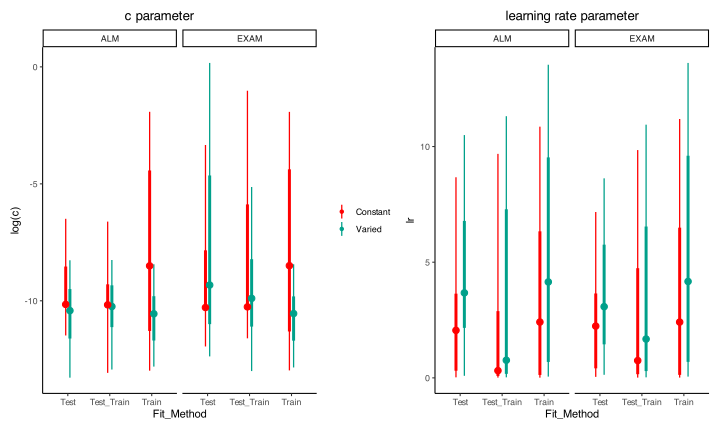
\includegraphics{full_files/figure-pdf/fig-htw-post-dist-1.pdf}

}

\caption{\label{fig-htw-post-dist}Posterior Distributions of \(c\) and
\(lr\) parameters. Points represent median values, thicker intervals
represent 66\% credible intervals and thin intervals represent 95\%
credible intervals around the median. Note that the y axes of the plots
for the c parameter are scaled logarithmically.}

\end{figure}%

\begin{figure}

\centering{

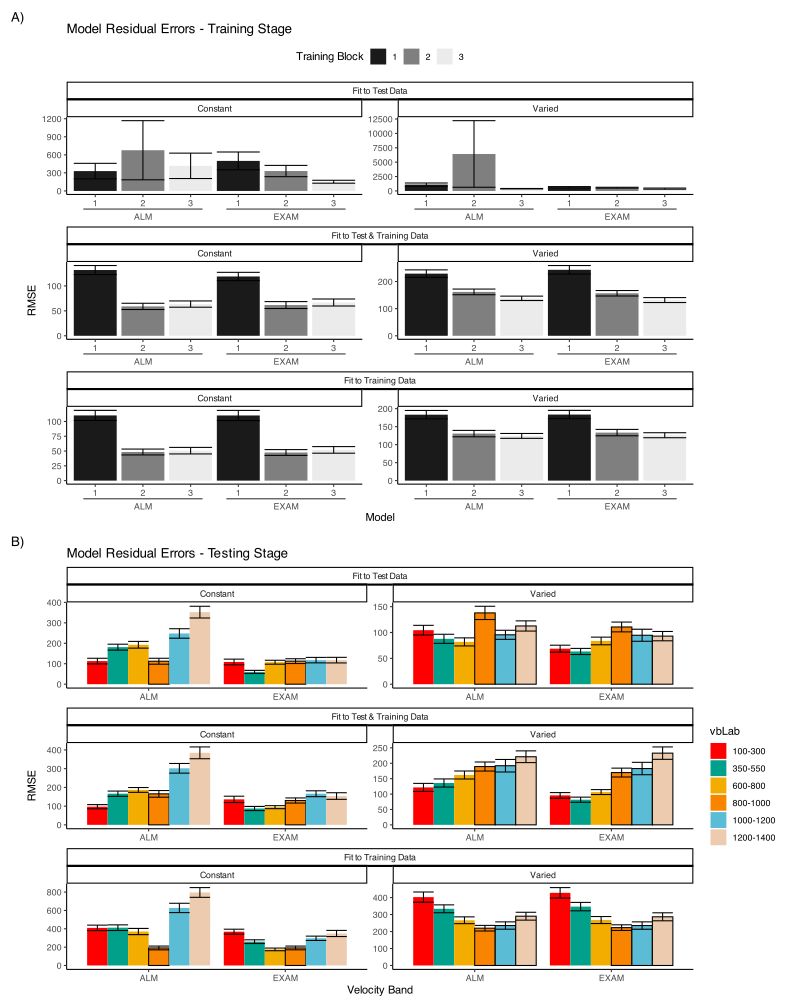
\includegraphics{full_files/figure-pdf/fig-htw-resid-pred-1.pdf}

}

\caption{\label{fig-htw-resid-pred}Model residuals for each combination
of training condition, fit method, and model. Residuals reflect the
difference between observed and predicted values. Lower values indicate
better model fit. Note that y axes are scaled differently between
facets. A) Residuals predicting each block of the training data. B)
Residuals predicting each band during the testing stage. Bolded bars
indicate bands that were trained, non-bold bars indicate extrapolation
bands.}

\end{figure}%

The posterior distributions of the \(c\) and \(lr\) parameters are shown
Figure~\ref{fig-htw-post-dist}, and model predictions are shown
alongside the empirical data in Figure~\ref{fig-cm-vx-pat}. There were
substantial individual differences in the posteriors of both parameters,
with the within-group individual differences generally swamped any
between-group or between-model differences. The magnitude of these
individual differences remains even if we consider only the single best
parameter set for each subject.

We used the posterior distribution of \(c\) and \(lr\) parameters to
generate a posterior predictive distribution of the observed data for
each participant, which then allows us to compare the empirical data to
the full range of predictions from each model. Aggregated residuals are
displayed in Figure~\ref{fig-htw-resid-pred}. The pattern of training
stage residual errors are unsurprising across the combinations of models
and fitting method . Differences in training performance between ALM and
EXAM are generally minor (the two models have identical learning
mechanisms). The differences in the magnitude of residuals across the
three fitting methods are also straightforward, with massive errors for
the `fit to Test Only' model, and the smallest errors for the `fit to
train only' models. It is also noteworthy that the residual errors are
generally larger for the first block of training, which is likely due to
the initial values of the ALM weights being unconstrained by whatever
initial biases participants tend to bring to the task. Future work may
explore the ability of the models to capture more fine grained aspects
of the learning trajectories. However for the present purposes, our
primary interest is in the ability of ALM and EXAM to account for the
testing patterns while being constrained, or not constrained, by the
training data. All subsequent analyses and discussion will thus focus on
the testing stage.

The residuals of the model predictions for the testing stage
(Figure~\ref{fig-htw-resid-pred}) also show an unsurprising pattern
across fitting methods - with models fit only to the test data showing
the best performance, followed by models fit to both training and test
data, and with models fit only to the training data showing the worst
performance (note that y axes are scaled different between plots).
Although EXAM tends to perform better for both Constant and Varied
participants (see also Figure~\ref{fig-ee-e1}), the relative advantage
of EXAM is generally larger for the Constant group - a pattern
consistent across all three fitting methods. The primary predictive
difference between ALM and EXAM is made clear in
Figure~\ref{fig-cm-vx-pat}, which directly compares the observed data
against the posterior predictive distributions for both models.
Regardless of how the models are fit, only EXAM can capture the pattern
where participants are able to discriminate all 6 target bands.

\begin{figure}

\centering{

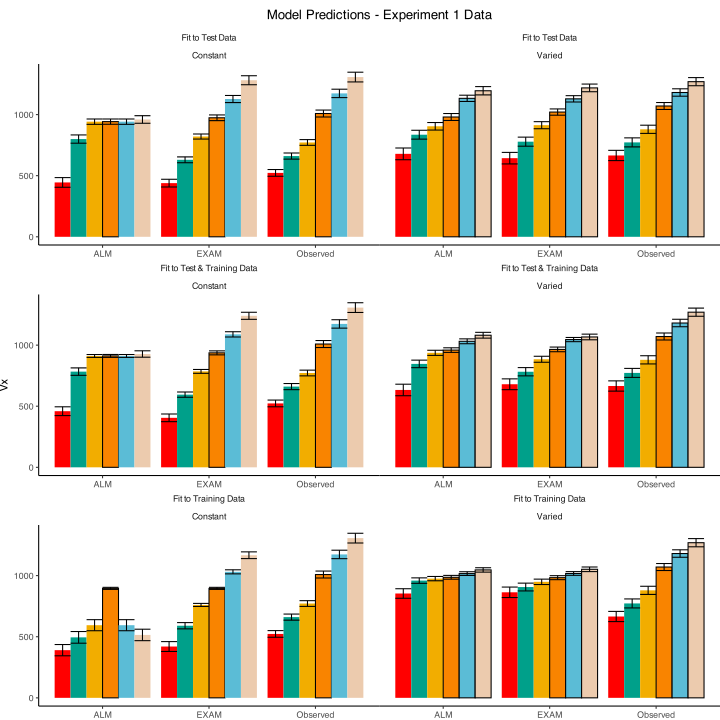
\includegraphics{full_files/figure-pdf/fig-cm-vx-pat-1.pdf}

}

\caption{\label{fig-cm-vx-pat}Empirical data and Model predictions for
mean velocity across target bands. Fitting methods (Test Only, Test \&
Train, Train Only) - are separated across rows, and Training Condition
(Constant vs.~Varied) are separated by columns. Each facet contains the
predictions of ALM and EXAM, alongside the observed data.}

\end{figure}%

\begin{figure}

\centering{

\captionsetup{labelsep=none}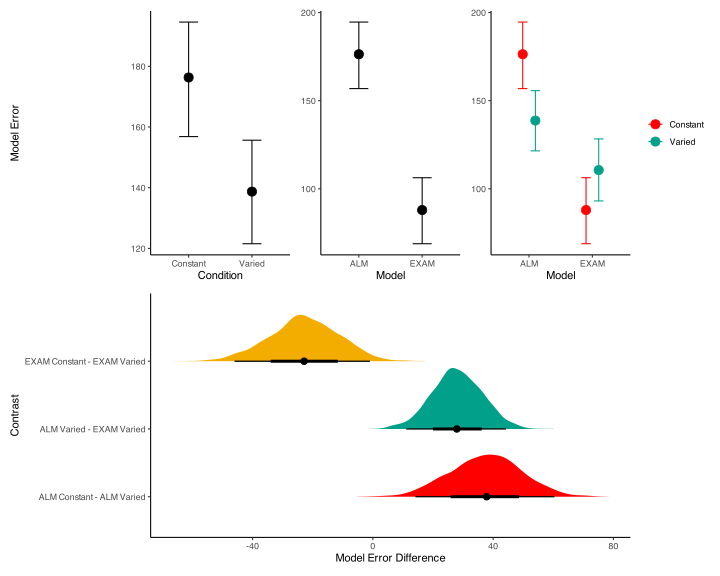
\includegraphics{full_files/figure-pdf/fig-ee-e1-1.pdf}

}

\caption{\label{fig-ee-e1}}

\end{figure}%

To quantitatively assess whether the differences in performance between
models, we fit a bayesian regressions predicting the errors of the
posterior predictions of each models as a function of the Model (ALM
vs.~EXAM) and training condition (Constant vs.~Varied).

Model errors were significantly lower for EXAM (\(\beta\) = -37.54, 95\%
CrI {[}-60.4, -14.17{]}, pd = 99.85\%) than ALM. There was also a
significant interaction between Model and Condition (\(\beta\) = 60.42,
95\% CrI {[}36.17, 83.85{]}, pd = 100\%), indicating that the advantage
of EXAM over ALM was significantly greater for the constant group. To
assess whether EXAM predicts constant performance significantly better
for Constant than for Varied subjects, we calculated the difference in
model error between the Constant and Varied conditions specifically for
EXAM. The results indicated that the model error for EXAM was
significantly lower in the Constant condition compared to the Varied
condition, with a mean difference of -22.88 (95\% CrI {[}-46.02,
-0.97{]}, pd = 0.98).

\begin{longtable}{lrrrrrrrr}

\caption{\label{tbl-htw-modelError-e23}Models errors predicting
empirical data - aggregated over all participants, posterior parameter
values, and velocity bands. Note that Fit Method refers to the subset of
the data that the model was trained on, while Task Stage refers to the
subset of the data that the model was evaluated on.}

\tabularnewline

\toprule
 & \multicolumn{4}{c}{E2} & \multicolumn{4}{c}{E3} \\ 
\cmidrule(lr){2-5} \cmidrule(lr){6-9}
 & \multicolumn{2}{c}{ALM} & \multicolumn{2}{c}{EXAM} & \multicolumn{2}{c}{ALM} & \multicolumn{2}{c}{EXAM} \\ 
\cmidrule(lr){2-3} \cmidrule(lr){4-5} \cmidrule(lr){6-7} \cmidrule(lr){8-9}
Task Stage & Constant & Varied & Constant & Varied & Constant & Varied & Constant & Varied \\ 
\midrule\addlinespace[2.5pt]
\multicolumn{9}{l}{Fit to Test Data} \\ 
\midrule\addlinespace[2.5pt]
\cellcolor[HTML]{FFFFFF}{Test} & \cellcolor[HTML]{FFFFFF}{$239.7$} & \cellcolor[HTML]{FFFFFF}{$129.8$} & \cellcolor[HTML]{FFFFFF}{$99.7$} & \cellcolor[HTML]{FFFFFF}{$88.2$} & \cellcolor[HTML]{FFFFFF}{$170.1$} & \cellcolor[HTML]{FFFFFF}{$106.1$} & \cellcolor[HTML]{FFFFFF}{$92.3$} & \cellcolor[HTML]{FFFFFF}{$72.8$} \\ 
\cellcolor[HTML]{FFFFFF}{Train} & \cellcolor[HTML]{FFFFFF}{$53.1$} & \cellcolor[HTML]{FFFFFF}{$527.1$} & \cellcolor[HTML]{FFFFFF}{$108.1$} & \cellcolor[HTML]{FFFFFF}{$169.3$} & \cellcolor[HTML]{FFFFFF}{$70.9$} & \cellcolor[HTML]{FFFFFF}{$543.5$} & \cellcolor[HTML]{FFFFFF}{$157.8$} & \cellcolor[HTML]{FFFFFF}{$212.7$} \\ 
\midrule\addlinespace[2.5pt]
\multicolumn{9}{l}{Fit to Test \& Training Data} \\ 
\midrule\addlinespace[2.5pt]
\cellcolor[HTML]{FFFFFF}{Test} & \cellcolor[HTML]{FFFFFF}{$266.0$} & \cellcolor[HTML]{FFFFFF}{$208.2$} & \cellcolor[HTML]{FFFFFF}{$125.1$} & \cellcolor[HTML]{FFFFFF}{$126.4$} & \cellcolor[HTML]{FFFFFF}{$197.7$} & \cellcolor[HTML]{FFFFFF}{$189.5$} & \cellcolor[HTML]{FFFFFF}{$130.0$} & \cellcolor[HTML]{FFFFFF}{$128.5$} \\ 
\cellcolor[HTML]{FFFFFF}{Train} & \cellcolor[HTML]{FFFFFF}{$40.0$} & \cellcolor[HTML]{FFFFFF}{$35.4$} & \cellcolor[HTML]{FFFFFF}{$30.4$} & \cellcolor[HTML]{FFFFFF}{$23.6$} & \cellcolor[HTML]{FFFFFF}{$49.1$} & \cellcolor[HTML]{FFFFFF}{$85.6$} & \cellcolor[HTML]{FFFFFF}{$49.2$} & \cellcolor[HTML]{FFFFFF}{$78.4$} \\ 
\midrule\addlinespace[2.5pt]
\multicolumn{9}{l}{Fit to Training Data} \\ 
\midrule\addlinespace[2.5pt]
\cellcolor[HTML]{FFFFFF}{Test} & \cellcolor[HTML]{FFFFFF}{$357.4$} & \cellcolor[HTML]{FFFFFF}{$295.9$} & \cellcolor[HTML]{FFFFFF}{$305.1$} & \cellcolor[HTML]{FFFFFF}{$234.5$} & \cellcolor[HTML]{FFFFFF}{$415.0$} & \cellcolor[HTML]{FFFFFF}{$298.8$} & \cellcolor[HTML]{FFFFFF}{$295.5$} & \cellcolor[HTML]{FFFFFF}{$243.7$} \\ 
\cellcolor[HTML]{FFFFFF}{Train} & \cellcolor[HTML]{FFFFFF}{$42.5$} & \cellcolor[HTML]{FFFFFF}{$23.0$} & \cellcolor[HTML]{FFFFFF}{$43.2$} & \cellcolor[HTML]{FFFFFF}{$22.6$} & \cellcolor[HTML]{FFFFFF}{$51.4$} & \cellcolor[HTML]{FFFFFF}{$63.8$} & \cellcolor[HTML]{FFFFFF}{$51.8$} & \cellcolor[HTML]{FFFFFF}{$65.3$} \\ 
\bottomrule

\end{longtable}

\begin{figure}

\centering{

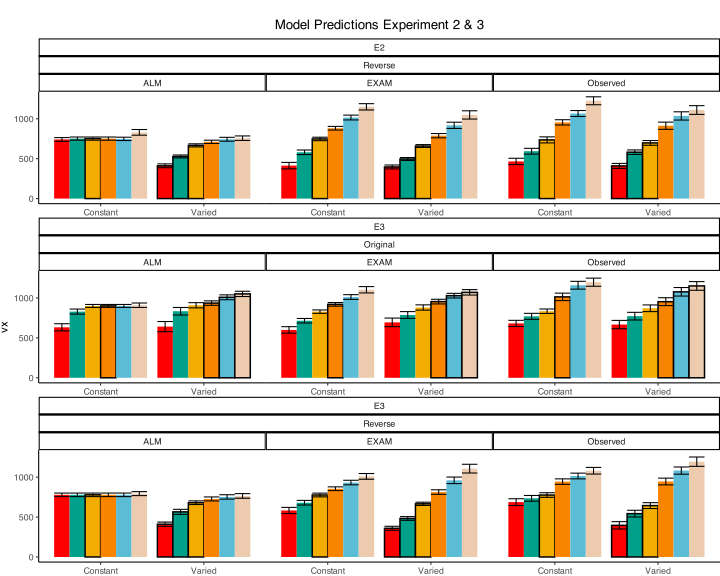
\includegraphics{full_files/figure-pdf/fig-cm-vx-pat-e2-e3-1.pdf}

}

\caption{\label{fig-cm-vx-pat-e2-e3}Empirical data and Model predictions
from Experiment 2 and 3 for the testing stage. Observed data is shown on
the right. Bolded bars indicate bands that were trained, non-bold bars
indicate extrapolation bands.}

\end{figure}%

\begin{longtable}{llrrrr}

\caption{\label{tbl-htw-ee-e23}Results of Bayesian Regression models
predicting model error as a function of Model (ALM vs.~EXAM), Condition
(Constant vs.~Varied), and the interaction between Model and Condition.
The values represent the estimate coefficient for each term, with 95\%
credible intervals in brackets. The intercept reflects the baseline of
ALM and Constant. The other estimates indicate deviations from the
baseline for the EXAM mode and varied condition. Lower values indicate
better model fit.}

\tabularnewline

\toprule
 &  &  & \multicolumn{2}{c}{Credible Interval} &  \\ 
\cmidrule(lr){4-5}
Experiment & Term & Estimate & 95\% CrI Lower & 95\% CrI Upper & pd \\ 
\midrule\addlinespace[2.5pt]
\multicolumn{6}{l}{Experiment 1} \\ 
\midrule\addlinespace[2.5pt]
Exp 1 & Intercept & $176.30$ & $156.86$ & $194.59$ & $1.00$ \\ 
Exp 1 & ModelEXAM & $-88.44$ & $-104.51$ & $-71.81$ & $1.00$ \\ 
Exp 1 & conditVaried & $-37.54$ & $-60.40$ & $-14.17$ & $1.00$ \\ 
Exp 1 & ModelEXAM:conditVaried & \cellcolor[HTML]{FFFFFF}{\textbf{$60.42$}} & $36.17$ & $83.85$ & \cellcolor[HTML]{FFFFFF}{\textbf{$1.00$}} \\ 
\midrule\addlinespace[2.5pt]
\multicolumn{6}{l}{Experiment 2} \\ 
\midrule\addlinespace[2.5pt]
Exp 2 & Intercept & $245.87$ & $226.18$ & $264.52$ & $1.00$ \\ 
Exp 2 & ModelEXAM & $-137.73$ & $-160.20$ & $-115.48$ & $1.00$ \\ 
Exp 2 & conditVaried & $-86.39$ & $-113.52$ & $-59.31$ & $1.00$ \\ 
Exp 2 & ModelEXAM:conditVaried & \cellcolor[HTML]{FFFFFF}{\textbf{$56.87$}} & $25.26$ & $88.04$ & \cellcolor[HTML]{FFFFFF}{\textbf{$1.00$}} \\ 
\midrule\addlinespace[2.5pt]
\multicolumn{6}{l}{Experiment 3} \\ 
\midrule\addlinespace[2.5pt]
Exp 3 & Intercept & $164.83$ & $140.05$ & $189.44$ & $1.00$ \\ 
Exp 3 & ModelEXAM & $-65.66$ & $-85.97$ & $-46.02$ & $1.00$ \\ 
Exp 3 & conditVaried & $-40.61$ & $-75.90$ & $-3.02$ & $0.98$ \\ 
Exp 3 & bandOrderReverse & $25.47$ & $-9.34$ & $58.68$ & $0.93$ \\ 
Exp 3 & ModelEXAM:conditVaried & \cellcolor[HTML]{FFFFFF}{\textbf{$41.90$}} & $11.20$ & $72.54$ & \cellcolor[HTML]{FFFFFF}{\textbf{$0.99$}} \\ 
Exp 3 & ModelEXAM:bandOrderReverse & $-7.32$ & $-34.53$ & $21.05$ & $0.70$ \\ 
Exp 3 & conditVaried:bandOrderReverse & $30.82$ & $-19.57$ & $83.56$ & $0.88$ \\ 
Exp 3 & ModelEXAM:conditVaried:bandOrderReverse & $-60.60$ & $-101.80$ & $-18.66$ & $1.00$ \\ 
\bottomrule

\end{longtable}

\emph{Model Fits to Experiment 2 and 3.} Data from Experiments 2 and 3
were fit to ALM and EXAM in the same manner as Experiment1 . For
brevity, we only plot and discuss the results of the ``fit to training
and testing data'' models - results from the other fitting methods can
be found in the appendix. The model fitting results for Experiments 2
and 3 closely mirrored those observed in Experiment 1. The Bayesian
regression models predicting model error as a function of Model (ALM
vs.~EXAM), Condition (Constant vs.~Varied), and their interaction (see
Table~\ref{tbl-htw-ee-e23}) revealed a consistent main effect of Model
across all three experiments. The negative coefficients for the
ModelEXAM term (Exp 2: \(\beta\) = -86.39, 95\% CrI -113.52, -59.31, pd
= 100\%; Exp 3: \(\beta\) = -40.61, 95\% CrI -75.9, -3.02, pd = 98.17\%)
indicate that EXAM outperformed ALM in both experiments. Furthermore,
the interaction between Model and Condition was significant in both
Experiment 2 (\(\beta\) = 56.87, 95\% CrI 25.26, 88.04, pd = 99.98\%)
and Experiment 3 (\(\beta\) = 41.9, 95\% CrI 11.2, 72.54, pd = 99.35\%),
suggesting that the superiority of EXAM over ALM was more pronounced for
the Constant group compared to the Varied group, as was the case in
Experiment 1. Recall that Experiment 3 included participants in both the
original and reverse order conditions - and that this manipulation
interacted with the effect of training condition. We thus also
controleld for band order in our Bayesian Regression assessing the
relative performance of EXAM and ALM in Experiment 3. There was a
significant three way interaction between Model, Training Condition, and
Band Order (\(\beta\) = -60.6, 95\% CrI -101.8, -18.66, pd = 99.83\%),
indicating that the relative advantage of EXAM over ALM was only more
pronounced in the original order condition, and not the reverse order
condition (see Figure~\ref{fig-e2_e3_ae}).

\begin{figure}

\centering{

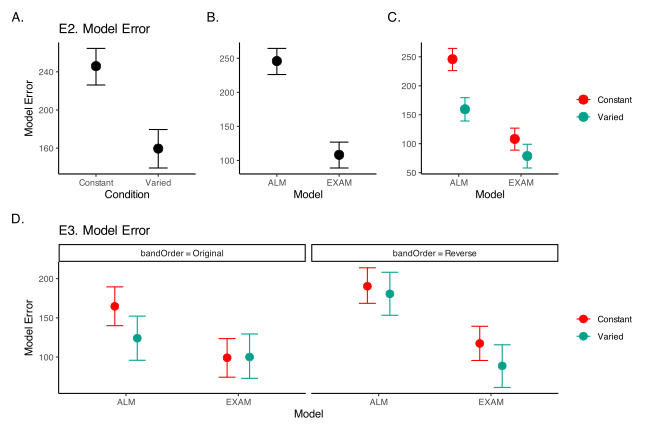
\includegraphics{full_files/figure-pdf/fig-e2_e3_ae-1.pdf}

}

\caption{\label{fig-e2_e3_ae}Conditional effects of Model (ALM vs EXAM)
and Condition (Constant vs.~Varied) on Model Error for Experiment 2 and
3 data. Experiment 3 also includes a control for the order of training
vs.~testing bands (original order vs.~reverse order).}

\end{figure}%

\emph{Computational Model Summary}. Across the model fits to all three
experiments, we found greater support for EXAM over ALM (negative
coefficients on the ModelEXAM term in Table~\ref{tbl-htw-ee-e23}), and
moreover that the constant participants were disproportionately well
described by EXAM in comparison to ALM (positive coefficients on
ModelEXAM:conditVaried terms in Table~\ref{tbl-htw-ee-e23}). This
pattern is also clearly depicted in Figure~\ref{fig-htw-best-model},
which plots the difference in model errors between ALM and EXAM for each
individual participant. Both varied and constant conditions have a
greater proportion of subjects better fit by EXAM (positive error
differences), with the magnitude of EXAM's advantage visibly greater for
the constant group. It also bears mention that numerous participants
were better fit by ALM, or did not show a clear preference for either
model. A subset of these participants are shown in
Figure~\ref{fig-htw-indv-pred}.

\begin{figure}

\centering{

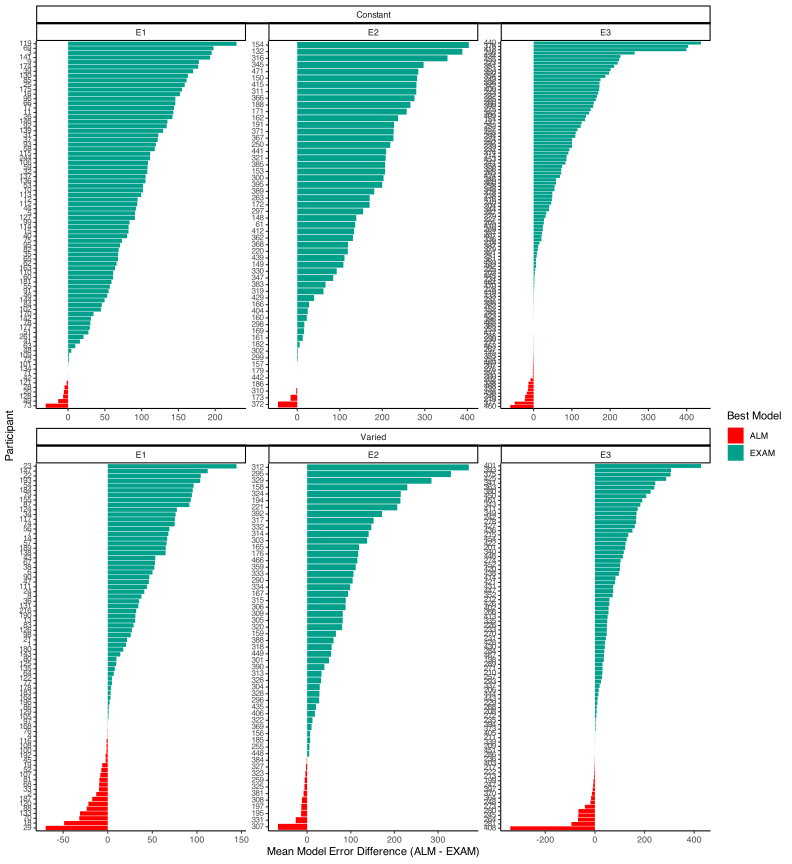
\includegraphics{full_files/figure-pdf/fig-htw-best-model-1.pdf}

}

\caption{\label{fig-htw-best-model}Difference in model errors for each
participant, with models fit to both train and test data. Positive
values favor EXAM, while negative values favor ALM.}

\end{figure}%

\begin{figure}

\centering{

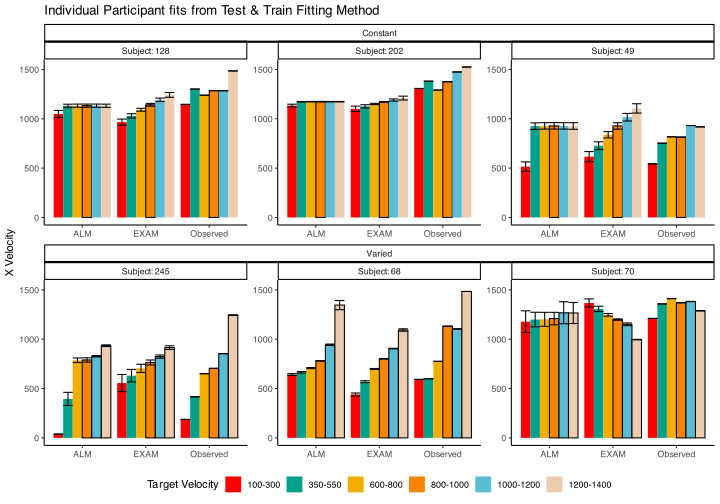
\includegraphics{full_files/figure-pdf/fig-htw-indv-pred-1.pdf}

}

\caption{\label{fig-htw-indv-pred}Model predictions alongside observed
data for a subset of individual participants. A) 3 constant and 3 varied
participants fit to both the test and training data. B) 3 constant and 3
varied subjects fit to only the trainign data. Bolded bars indicate
bands that were trained, non-bold bars indicate extrapolation bands.}

\end{figure}%

\section{General Discussion}\label{general-discussion-1}

\emph{Experimental Result Summary}

Across three experiments, we investigated the impact of training
variability on learning and extrapolation in a visuomotor function
learning task. In Experiment 1, participants in the varied training
condition, who experienced a wider range of velocity bands during
training, showed lower accuracy at the end of training compared to those
in the constant training condition.

Crucially, during the testing phase, the varied group exhibited
significantly larger deviations from the target velocity bands,
particularly for the extrapolation bands that were not encountered
during training. The varied group also showed less discrimination
between velocity bands, as evidenced by shallower slopes when predicting
response velocity from target velocity band.

Experiment 2 extended these findings by reversing the order of the
training and testing bands. Similar to Experiment 1, the varied group
demonstrated poorer performance during both training and testing phases.
However, unlike Experiment 1, the varied group did not show a
significant difference in discrimination between bands compared to the
constant group.

In Experiment 3, we provided only ordinal feedback during training, in
contrast to the continuous feedback provided in the previous
experiments. Participants were assigned to both an order condition
(original or reverse) and a training condition (constant or varied). The
varied condition showed larger deviations at the end of training,
consistent with the previous experiments. Interestingly, there was a
significant interaction between training condition and band order, with
the varied condition showing greater accuracy in the reverse order
condition. During testing, the varied group once again exhibited larger
deviations, particularly for the extrapolation bands. The reverse order
conditions showed smaller deviations compared to the original order
conditions. Discrimination between velocity bands was poorer for the
varied group in the original order condition, but not in the reverse
order condition.

All three of our experiments yielded evidence that varied training
conditions produced less learning by the end of training, a pattern
consistent with much of the previous research on the influence of
training variability
\autocite{catalanoDistantTransferCoincident1984a,wrisbergVariabilityPracticeHypothesis1987,soderstromLearningPerformanceIntegrative2015}.
The sole exception to this pattern was the reverse order condition in
Experiment 3, where the varied group was not significantly worse than
the constant group. Neither the varied condition trained with the same
reverse-order items in Experiment 2, nor the original-order varied
condition trained with ordinal feedback in Experiment 3 were able to
match the performance of their complementary constant groups by the end
of training, suggesting that the relative success of the ordinal-reverse
ordered varied group cannot be attributed to item or feedback effects
alone.

Our findings also diverge from the two previous studies to cleanly
manipulate the variability of training items in a function learning task
\autocite{deloshExtrapolationSineQua1997,vandamMappingShapeVisuomotor2015},
although the varied training condition of
\textcite{vandamMappingShapeVisuomotor2015} also exhibited less
learning, neither of these previous studies observed any difference
between training conditions in extrapolation to novel items. Like
\textcite{deloshExtrapolationSineQua1997} , our participants exhibited
above chance extrapolation/discrimination of novel items, however they
observed no difference between any of their three training conditions. A
noteworthy difference difference between our studies is that
\textcite{deloshExtrapolationSineQua1997} trained participants with
either 8, 20, or 50 unique items (all receiving the same total number of
training trials). These larger sets of unique items, combined with the
fact that participants achieved near ceiling level performance by the
end of training - may have made it more difficult to observe any
between-group differences of training variation in their study.
\textcite{vandamMappingShapeVisuomotor2015} 's variability manipulation
was more similar to our own, as they trained participants with either 2
or 5 unique items. However, although the mapping between their input
stimuli and motor responses was technically linear, the input dimension
was more complex than our own, as it was defined by the degree of
``spikiness'' of the input shape. This entirely arbitrary mapping also
would have preculded any sense of a ``0'' point, which may partially
explain why neither of their training conditions were able to
extrapolate linearly in the manner observed in the current study or in
\textcite{deloshExtrapolationSineQua1997}.

\emph{Modeling Summary} EXAM is the best model for both groups, but EXAM
does relatively good at accounting for the constant group. May have
seemed counterintuitive, if one assumed that multiple, varied, examples
were necessary to extract a rule. But, EXAM is not a conventional rule
model - it doesn't require explictly abstract of a rule, but rather the
rule-based response occurs during retrieval. The constant groups
formation of a single, accurate, input-output association, in
combination with the usefulness of the zero point, may have been
sufficient for EXAM, and the constant group, to perform well. One
concern may have been that the assumption of participants making use of
the zero point turned the extrapolation problem into an interpolation
problem - however this concern is ameliorated by the consistency of the
results across both the original and reverse order conditions.

\emph{Limitations}

While the present study provides valuable insights into the influence of
training variability on visuomotor function learning and extrapolation,
there are several limitations that should be flagged. First, although
the constant training group never had experience from a velocity band
closer to the extrapolation bands than the varied group, they always had
a three times more trials with the nearest velocity band. Such a
difference may be an unavoidable consequence of varied vs.~constant
design which match the total number of training trials between the two
groups. However in order to more carefully tease apart the influence of
variability from the influence of frequency/repetition effects, future
research could explore alternative designs that maintain the variability
manipulation while equating the amount of training on the nearest
examples across conditions, such as by increasing the total number of
trials for the varied group. Another limitation is that the testing
stage did not include any interpolation items, i.e.~the participants
tested only from the training bands they experienced during training, or
from extrapolation bands. The absence of interpolation testing makes it
more difficult to distinguish between the effects of training
variability on extrapolation specifically, as opposed to generalization
more broadly. Of course, the nature of the constant training condition
makes interpolation teseting impossible to implement, however future
studies might compare a training regimes that each include at least 2
distinct items, but still differ in total amount of variability
experienced, which would then allow groups to be compared in terms of
both interpolation and extrapolation testing. Finally, the task employed
in the present study consisted of only a linear, positive function.
Previous work in human function learning has repeatedly shown that such
functions are among the easiest to learn, but that humans are
nonetheless capable of learning negative, non-linear, or discontinuous
functions
\autocite{deloshExtrapolationSineQua1997,mcdanielPredictingTransferPerformance2009,kalishLearningExtrapolatingPeriodic2013,busemeyerLearningFunctionalRelations1997}.
It thus remains an open question as to whether the influence of training
variability might interact with various components of the to-be-learned
function.

\subsection{Comparison to Project 1}\label{comparison-to-project-1}

\subsubsection{Differences between the
tasks}\label{differences-between-the-tasks}

There are a number of differences between Project 1's Hit The Target
(HTT), and Project 2's Hit The Wall (HTW) tasks.

\begin{itemize}
\item
  Task Space Complexity: In~HTW,~the task space is also almost perfectly
  smooth, at least for the continuous feedback subjects, if they throw
  100 units too hard, they'll be told that they were 100 units too hard.
  Whereas in HTT, ~it was possible to produce xy velocity combinations
  that were technically closer to the empirical solution space than
  other throws, but which resulted in worse feedback due to striking the
  barrier.
\item
  Perceptual Distinctiveness: HTT offers perceptually distinct varied
  conditions that directly relate to the task's demands, which may
  increase the sallience between training positions encounted by the
  varied group. In contrast, HTW's varied conditions differ only in the
  numerical values displayed, lacking the same level of perceptual
  differentiation. Conversely in~HTW, the only difference between
  conditions for the varied group are the numbers displayed at the top
  of the screen which indicate the current target band(e.g.~800-1000, or
  1000-1200)
\item
  In~HTW, our primary testing stage of interest has no feedback, whereas
  in HTT testing always included feedback (the intermittent testing in
  HTT expt 1 being the only exception). Of course, we do collect testing
  with feedback data at the end of~HTW, but we haven't focused on that
  data at all in our modelling work thus far. It's also interesting to
  recall that the gap between varied and constant in~HTW~does seem to
  close substantially in the testing-with-feedback stage. The difference
  between no-feedback and feedback testing might be relevant if the
  benefits of variation have anything to do with improving subsequent
  learning (as opposed to subsequent immediate performance), OR if the
  benefits of constant training rely on having the most useful anchor,
  having the most useful anchor might be a lot less helpful if you're
  getting feedback from novel positions and can thus immediately begin
  to form position-specific anchors for the novelties, rather than
  relying on a training anchor.~
\item
  HTW~and HTT both have a similar amount of training trials
  (\textasciitilde200), and thus the constant groups acquire a similar
  amount of experience with their single position/velocity in both
  experiments. However, the varied conditions in both HTT
  experiments~train on 2 positions, whereas the varied group
  in~HTW~trains on 3 velocity bands. This means that in HTT the varied
  group gets half as much experience on any one position as the constant
  group, and in~HTW~they only get 1/3 as much experience in any one
  position. There are likely myriad ways in which this might impact the
  success of the varied group regardless of how you think the benefits
  of variation might be occurring, e.g.~maybe they also need to develop
  a coherent anchor, maybe they need more experience in order to extract
  a function, or more experience in order to properly learn to tune
  their c parameter.~
\end{itemize}

\section{References}\label{references}

%bib-loc-124C8010

\section{Appendix}\label{appendix}

Reviewer \#2: This study addresses a question that is important both
theoretically and practically. However, the authors need to rule out the
following, less interesting alternative. Namely, the results could be
due to task practice effect, as follows.

Since there was no pre-training test, and no practice trials (as far as
I can tell), and since the task was an online motor task that
participants could not rely on their prior motor experience, trying to
launch the ball to the target could only be done via trial and error.
For the varied training group, they got to practice at two distances.
Therefore, they had a better ``calibration'' in terms of the
relationship between launching speed and target distance. This was
likely beneficial both in Exp.1 when both transfer distances were
interpolations from the two trained distances, and in Exp.2 when two
transfer distances were interpolations and two were extrapolations but
the latter two were immediately next to the training distances.

In comparison, since the constant group trained at only a single
distance, any transfer distance (or at least the first transfer distance
tested) was extrapolation even if this transfer distance was shorter
than the trained, because the participants did not know beforehand how
to shoot the ball to the shortest distance due to the existence of the
barrier. If the transfer distance was longer, for sure that was
extrapolation.

Regardless, the above analysis suggests that the constant group would
always be a step behind the varied group. The number of trials at each
transfer distance may not be sufficient for them to catch up the varied
group either (whether there was learning during testing should be
checked). If such disadvantage for the constant group is indeed due to
the lack of tryout opportunities, then the authors should verify whether
the same results still hold if all groups were provided opportunities to
practice, or if pre-training tests across all distances were offered.

\subsubsection{exponential learning models fit to individual
subjects}\label{exponential-learning-models-fit-to-individual-subjects}

\subsubsection{Group comparison of learning rate
fits}\label{group-comparison-of-learning-rate-fits}

\includegraphics{full_files/figure-pdf/unnamed-chunk-60-1.pdf}

\subsubsection{First vs.~second half of testing
stage}\label{first-vs.-second-half-of-testing-stage}

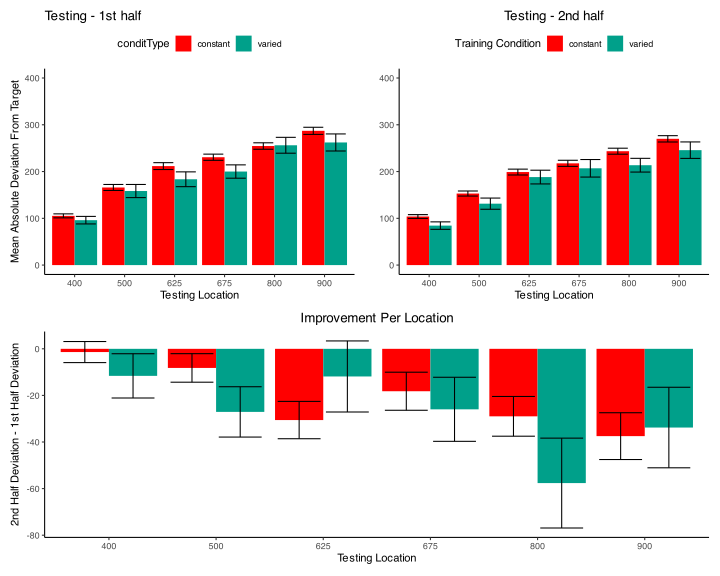
\includegraphics{full_files/figure-pdf/unnamed-chunk-61-1.pdf}

\subsubsection{Group Comparison for asymptote-starting
performance}\label{group-comparison-for-asymptote-starting-performance}

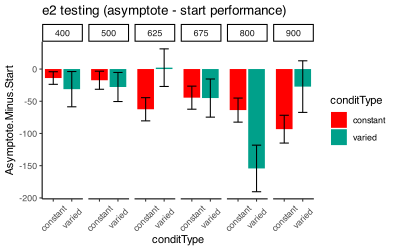
\includegraphics{full_files/figure-pdf/unnamed-chunk-62-1.pdf}

\subsubsection{Relative distance and
under/overshooting}\label{relative-distance-and-underovershooting}

Reviewer 3 Absolute versus relative distance: From a methodological
standpoint, I understand the need to differentiate these two types of
distance. However, from a theoretical perspective there may be some
issue in differentiating these two concepts. Schema theory relies on
relative (or invariant) information to inform the motor program.
However, both distances would be important to an instance or exemplar
representation. You may want to consider commenting on this issue.

Reviewer 2 For the same reason, the plots showing improvement during
training could be due to participants learning the task, rather than
fine motor skills. Although task learning and motor learning are
impossible to separate cleanly, the common practice in the field is
indeed to offer practice trials to reduce the task learning aspects. The
authors should address this.

In addition to absolute errors (which is related to variance), the
authors should also provide other measures of performance, e.g., the
mean of the signed errors, so that readers have a better idea whether
there was any meaningful over- or undershooting.

\paragraph{experiment 1 training - relative
distances}\label{experiment-1-training---relative-distances}

\includegraphics{full_files/figure-pdf/unnamed-chunk-63-1.pdf}

\includegraphics{full_files/figure-pdf/unnamed-chunk-63-2.pdf}

\includegraphics{full_files/figure-pdf/unnamed-chunk-63-3.pdf}

\includegraphics{full_files/figure-pdf/unnamed-chunk-63-4.pdf}

\begin{verbatim}

=========================================================================
conditType devianceDirection      610            760            910      
-------------------------------------------------------------------------
constant       Overshoot                    311.84(307.92)               
constant      Undershoot                    188.05(163.62)               
varied         Overshoot     211.69(234.97)                360.14(322.01)
varied        Undershoot     107.35(81.21)                 244.85(196.47)
-------------------------------------------------------------------------
\end{verbatim}

\begin{verbatim}

======================================================
conditType      610           760            910      
------------------------------------------------------
constant                 121.03(269.17)               
varied     39.91(178.12)                150.53(290.04)
------------------------------------------------------
\end{verbatim}

\begin{verbatim}

====================================================================
conditType     610           760            835            910      
--------------------------------------------------------------------
constant   7.13(124.02) 107.02(218.49) 142.42(252.34) 122.92(282.58)
varied     3.19(96.67)   92.1(173.9)   103.84(214.4)  108.12(234.59)
--------------------------------------------------------------------
\end{verbatim}

\paragraph{experiment 2 training - relative
distances}\label{experiment-2-training---relative-distances}

\includegraphics{full_files/figure-pdf/unnamed-chunk-64-1.pdf}

\includegraphics{full_files/figure-pdf/unnamed-chunk-64-2.pdf}

\paragraph{Experiment 1 Testing - relative
distances}\label{experiment-1-testing---relative-distances}

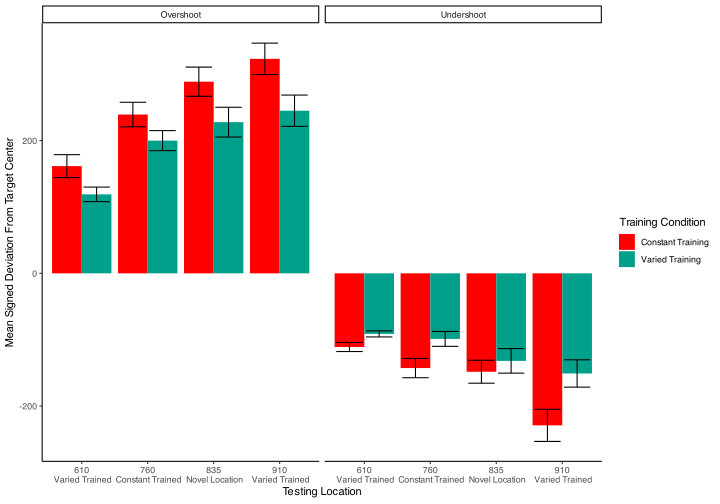
\includegraphics{full_files/figure-pdf/unnamed-chunk-65-1.pdf}

\begin{verbatim}

====================================================================================================================================
conditType2         msdu_610       msdu_760       msdu_835       msdu_910      msds_610      msds_760      msds_835      msds_910   
------------------------------------------------------------------------------------------------------------------------------------
Constant Training 136.27(84.29) 191.65(112.65) 219.46(139.91) 276.75(153.09) 25.28(158.98) 50.82(217.48) 73.14(250.93) 50.76(313.77)
Varied Training   105.12(51.39)  149.37(93.4)  180.54(129.52) 198.64(137.84) 13.85(116.87) 50.59(169.59) 50.52(217.39) 49.94(237.71)
------------------------------------------------------------------------------------------------------------------------------------
\end{verbatim}

\begin{verbatim}

=========================================================================
Condition              610           760           835           910     
-------------------------------------------------------------------------
Constant Training 25.28(158.98) 50.82(217.48) 73.14(250.93) 50.76(313.77)
Varied Training   13.85(116.87) 50.59(169.59) 50.52(217.39) 49.94(237.71)
-------------------------------------------------------------------------
\end{verbatim}

\paragraph{Experiment 2 Testing - relative
distances}\label{experiment-2-testing---relative-distances}

\includegraphics{full_files/figure-pdf/unnamed-chunk-66-1.pdf}

\paragraph{Experimenet 1 - intermittent
testing}\label{experimenet-1---intermittent-testing}

\includegraphics{full_files/figure-pdf/unnamed-chunk-67-1.pdf}

\begin{verbatim}

======================================================================================================
Condition 610_First Half 760_First Half 910_First Half 610_Second Half 760_Second Half 910_Second Half
------------------------------------------------------------------------------------------------------
constant  206.64(82.08)  286.51(121.07) 406.93(145.2)   187.2(55.24)    238.21(95.16)  313.27(114.86) 
varied    195.68(78.58)  278.9(105.37)  318.53(134.81)  177.79(70.82)  224.98(108.04)   276.86(110.5) 
------------------------------------------------------------------------------------------------------
\end{verbatim}

\subsubsection{Training plots - Experiment
1}\label{training-plots---experiment-1}

\includegraphics{full_files/figure-pdf/unnamed-chunk-68-1.pdf}

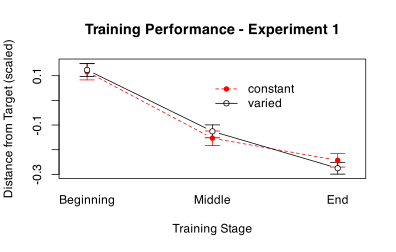
\includegraphics{full_files/figure-pdf/unnamed-chunk-68-2.pdf}

\includegraphics{full_files/figure-pdf/unnamed-chunk-68-3.pdf}

\paragraph{Not in manuscript}\label{not-in-manuscript}

\paragraph{fit to testing performance averaged across
positions}\label{fit-to-testing-performance-averaged-across-positions}

\includegraphics{full_files/figure-pdf/unnamed-chunk-69-1.pdf}

\includegraphics{full_files/figure-pdf/unnamed-chunk-69-2.pdf}

\includegraphics{full_files/figure-pdf/unnamed-chunk-69-3.pdf}

\paragraph{statistical tests for starting
performance}\label{statistical-tests-for-starting-performance}

\begin{verbatim}
ANOVA Table (type III tests)

      Effect DFn DFd F     p p<.05   ges
1 conditType   1 206 3 0.083       0.015
\end{verbatim}

\includegraphics{full_files/figure-pdf/unnamed-chunk-70-1.pdf}

\paragraph{statistical tests for
asymptote}\label{statistical-tests-for-asymptote}

\begin{verbatim}
ANOVA Table (type III tests)

      Effect DFn DFd   F     p p<.05   ges
1 conditType   1 206 3.4 0.067       0.016
\end{verbatim}

\includegraphics{full_files/figure-pdf/unnamed-chunk-71-1.pdf}


\printbibliography[title=References]


\end{document}
